% !TeX_ROOT=../../thesis.tex

%% !TeX_ROOT=../thesis.tex

\newcommand{\TODO}[1]{\todo[inline, color=orange!30]{\textbf{TODO:} #1}}
\newcommand{\Question}[1]{\todo[inline, color=red!30]{\textbf{Question:} #1}}



% Classical Spaces
\newcommand{\B}{\mathbb{B}}
\newcommand{\Z}{\mathbb{Z}}
\newcommand{\T}{\mathbb{T}}
\newcommand{\R}{\mathbb{R}}

% Distributions
\newcommand{\unif}[1]{\mathcal U \left ( #1 \right )}


% Problems / Ciphertexts
\newcommand{\LWE}{\textsf{LWE}}
\newcommand{\TrivialLWE}{\textsf{TrivialLWE}}
\newcommand{\RLWE}{\textsf{RLWE}}
\newcommand{\GLWE}{\textsf{GLWE}}
\newcommand{\GGSW}{\textsf{GGSW}}

% Classical Mathematical Operations
\newcommand{\rounding}[1]{\left \lfloor #1 \right \rceil}
\newcommand{\drawfrom}{\overset{\$}{\leftarrow}}



% TFHE-specific notations
\newcommand{\lweSigma}{\sigma_{\LWE}}
\newcommand{\glweSigma}{\sigma_{\GLWE}}
\newcommand{\baseDecomp}{B}
\newcommand{\levelDecomp}{\ell}


\newcommand{\lweSecretKey}{\vec s}
\newcommand{\glweSecretKey}{\vec S}

\newcommand{\BSK}{\textsf{BSK}} 
\newcommand{\KSK}{\textsf{KSK}} 
% TODO : trouver une otation pl^us jolie pour BSK


%TFHE homomorphic operations

\newcommand{\sumTFHE}[2]{\texttt{SumTFHE}(#1, #2)}
\newcommand{\sumTFHETernary}[3]{\texttt{SumTFHE}(#1, #2, #3)}
\newcommand{\sumTFHEQuad}[4]{\texttt{SumTFHE}(#1, #2, #3, #4)}
\newcommand{\clearMultTFHE}[2]{\texttt{ClearMultTFHE}(#1, #2)}

\newcommand{\squarewithdot}{\tikz[baseline=-0.5ex]\draw (0,0) rectangle (0.3,0.3) (0.15,0.15) circle (0.05);}

% other operations
\newcommand{\decomp}[3]{\textsf{dec}^{(#1, #2)}(#3)}

% TFHE-related spaces\\
\newcommand{\plaintextTorus}{\mathbb{T}_p}
\newcommand{\plaintextRing}{\mathbb{Z}_p}
\newcommand{\plaintextTorusPoly}{\mathbb{T}_p[X] / (X^N + 1)}
\newcommand{\plaintextRingPoly}{\mathbb{Z}_p[X] / (X^N + 1)}
\newcommand{\lweTorus}{\mathbb{T}_q}
\newcommand{\lweRing}{\mathbb{Z}_q}
\newcommand{\glweTorus}{\mathbb{T}_q[X] / (X^N + 1)}
\newcommand{\glweRing}{\mathbb{Z}_q[X] / (X^N + 1)}



% environments
\theoremstyle{definition}
\newtheorem{definition}{Definition}[section]


% components
\newcommand\plaintextSpace{\mathcal{P}}
\newcommand\mainField{\F_{p}}
\newcommand\evenRing{\mathbb{Z}_t}
\newcommand\LFSRlen{\text{\textsf{len}}}
\newcommand\pseudoKS{\mathcal{K}}
\newcommand\whitening{\mathcal{W}}
\newcommand\thesbox{\pi}
\newcommand\mixmat{M}
\newcommand\filter{\phi}
\newcommand\fsmState[1]{X_{#1}}

% noises
\newcommand\noiseFresh{\sigma_\text{\textsf{fresh}}}
\newcommand\noisePBS{\sigma_\text{\textsf{PBS}}}
\newcommand\noiseLFSR{\sigma_\text{\textsf{LFSR}}}
\newcommand\noiseBeforeSN{\sigma_\text{\textsf{SN}}}
\newcommand\noiseOutput{\sigma_\text{\textsf{output}}}

% operations
\newcommand\subWords{\text{\textsf{SubDigits}}}
\newcommand\mixColumns{\text{\textsf{MixColumns}}}
\newcommand\shiftRows{\text{\textsf{ShiftRows}}}
\newcommand\filterName{\text{\textsf{Filter}}}
\newcommand\subW{\text{\textsf{SD}}}
\newcommand\mixC{\text{\textsf{MC}}}
\newcommand\shiftR{\text{\textsf{SR}}}
\newcommand\clock[1]{\mathsf{clock}_{#1}}


% macros for proof
\newcommand\keyspace{\mathcal{K}}
\newcommand\outspace{\mathcal{S}}
\newcommand\keyevent{k}
\newcommand\outevent{s}
\newcommand\keyvar{K}
\newcommand\outvar{S}
\newcommand\fsmspace{\mathcal{X}}
\newcommand\fsmvar{X}
\newcommand{\set}[1]{\left\{#1\right\}}
\newcommand{\card}[1]{\left|#1\right|}
\newcommand{\hamming}{\mathrm{wt}}
\newcommand{\im}{\mathrm{Im}}


% Cool names
\newcommand\coolName{\texttt{Transistor}\xspace}
\newcommand\minimalLength{correlation-immune length\xspace}

% latex magic for eprint version
\newif\ifeprint
\eprinttrue
%\eprintfalse





In the previous chapter (Section \ref{sec:transciphering}), we have presented a technique called transciphering to adress the challenge of ciphertext expansion, common with all the FHE scheme. For example, a plaintext message of a few kilobytes can require tens or even hundreds of megabytes of data, making the processing of large data sets impractical. While compression techniques can help reduce the expansion factor in TFHE ciphertexts, the encrypted data still remains an order or two of magnitude larger than the original plaintext.


Transciphering consists in encrypting the data using a symmetric encryption cipher, and only encrypting the key of this cipher using the FHE scheme. Then, the server can evaluate the decryption algorithm of the symmetric cipher homomorphically to produce usable FHE ciphertexts. More information on transciphering is given in Section \ref{sec:transciphering}.


While \hippo, our implementation of homomorphic AES we introduced in previous chapter, could in theory be used for such transciphering task, the performances would not be acceptable for large volume of data (which is the use-case targeted by transciphering). We would rather have a symmetric cipher designed specifically to interact well with the FHE scheme. An abundant literature on the topic has appeared during the last few years, leading to the development of new families of ciphers tailored for the different homomorphic scheme on the market.


In this chapter, we present \coolName{}, a stream cipher optimized for transciphering with TFHE. This design is the outcome of a careful study of the constraints and advantages specific to achieving efficient homomorphic evaluations with TFHE. In particular, we argue that operating on elements of $\mathbb{F}_p$, where $p$ is a small prime (4--5 bits), is a good choice for leveraging the full potential of TFHE’s programmable bootstrapping: we chose $p=17$. This choice is independent of the data format supported by the application running on the server, as changes of representations are easily feasible through bootstrapping~\cite{JC:BBBCLO23}.


The design of \coolName has combined two very different challenges: ensuring security (in the sense of ``traditional'' cryptographic security), while being evaluable efficiently in the homomorphic domain. This thesis being about the development of efficient homomorphic operations, we mainly present the latter aspect in this chapter. A full version of this work is available in \cite{EPRINT:BBBBCL25}, giving a more complete vision of the other aspect of the design. In particular, we present a careful analysis of the noise evolution throughout  the homomorphic evaluation of \coolName, to fine-tune the TFHE parameters for optimal performance. Our homomorphic implementation of \coolName{} significantly outperforms the state of the art, achieving a throughput of over 60 bits/s on a standard CPU. This represents a factor 3 speedup compared to \texttt{FRAST}~\cite{ToSC:CCHLOS24}, the previous fastest method, while also achieving a considerably lower error probability and eliminating the need for an expensive initialization phase.


The chapter is structured as follows. Section~\ref{sec:constraints} discusses the design constraints for a stream cipher intended for use with TFHE, along with the design choices we made. The specification of \coolName{} and the reasoning behind its design is detailed in Section~\ref{sec:description}. Section~\ref{sec:security} provides a brief high-level summary of the security implications. Finally, Section~\ref{sec:bench} details the homomorphic implementation of our scheme, providing performance metrics and benchmarks.



\section{Constraints for a \gls{TFHE}-friendly Stream Cipher}
\label{sec:constraints}



%\subsection{State-of-the-Art}
%\label{sec:soa}
%
%While transciphering can theoretically be instantiated with any symmetric cipher, traditional ciphers like \gls{AES} were soon found to be suboptimal~\cite{C:GenHalSma12}, which lead to the design of dedicated ciphers.
%Early proposals in this direction include the {\tt LowMC} family of block ciphers~\cite{EC:ARSTZ15}, which minimizes multiplicative depth, and the {\tt Kreyvium} stream cipher~\cite{FSE:CCFLNP16}, a tweak of the well-known eSTREAM finalist {\tt Trivium}. While {\tt Trivium} itself was not originally designed for homomorphic encryption, both {\tt Trivium} and {\tt Kreyvium} showed competitive performance in \gls{TFHE}-based transciphering scenarios~\cite{DBLP:conf/wahc/BalenboisOS23}.
%
%In 2016, the {\tt FLIP} stream cipher~\cite{EC:MJSC16} introduced the concept of a filter permutator that randomly permutes key bits and applies a non-linear function on the result to generate a keystream bit. The direct application of non-linear filtering on low-noise key bits helps control the noise generated during homomorphic operations. Two variants were then proposed: {\tt FiLIP}~\cite{INDOCRYPT:MCJS19} and {\tt Elisabeth}~\cite{AC:CHMS22}, which aimed for stronger security and improved performance. Most notably, {\tt Elisabeth} operates over arbitrary groups like $\mathbb{Z}_{2^4}$ to minimize costly field conversions in homomorphic evaluations, and it leverages negacyclic lookup tables to eliminate padding bits, thereby optimizing \gls{TFHE} performance. However, in 2023, an algebraic attack successfully compromised {\tt Elisabeth}~\cite{AC:GBJR23}, prompting the design of patched versions: {\tt Elisabeth-b}, {\tt Gabriel}, and {\tt Margrethe}~\cite{INDOCRYPT:HofMeaSta23}. While these variants address the identified vulnerabilities, they introduce trade-offs in efficiency: either the evaluation cost or the communication overhead significantly increases compared to the original {\tt Elisabeth}.
%
%Another recent contribution is the construction of a PRF~\cite{EPRINT:DJLCB24} based on the Learning With Rounding (LWR) problem~\cite{EC:BanPeiRos12}. Computing one PRF output requires only a single \gls{PBS} in the \gls{TFHE} context. Still, the main overhead stems from the transmission of the secret key in GGSW format,\footnote{This technique is a generalization of the one introduced in~\cite{C:GenSahWat13}.}  which is significantly larger than traditional LWE ciphertexts.
%
%Finally, the {\tt FRAST} stream cipher~\cite{FRAST} is built on top of a block cipher with a \gls{TFHE}-friendly round function, %that leverages a random \gls{S-box} to enable a reduced number of rounds,
%and evaluates it efficiently using the double-blind rotation technique combined with \gls{WoP-PBS}. This allows multiple \gls{S-box} invocations to be processed at the cost of a single \gls{PBS}. {\tt FRAST} achieves substantial improvements in throughput while maintaining competitive noise growth. Its main trade-offs lie in a slight increase in communication cost and the need for an initial setup phase to convert GLWE ciphertexts into GGSW form~\cite{C:GenSahWat13}.
%
%Concrete performance figures for all the above-mentioned ciphers are provided in Section~\ref{sec:perfs_soa}.
%
 



%\subsection{Constraints from \gls{TFHE}}
%\label{constraints_tfhe}


\paragraph{\gls{TFHE} Operations.} \gls{TFHE} enables the evaluation of both linear functions and look-up tables on encrypted data, each offering complementary properties.

Linear operations in \gls{TFHE} are highly efficient but contribute to an increase in ciphertext noise. Specifically, when performing a linear combination of ciphertexts $c_1, \ldots, c_n$ with constant coefficients $\alpha_1, \ldots, \alpha_n$, the noise variance increases in proportion to the squared $\ell_2$-norm of the coefficient vector, i.e., $\sum_{i=1}^n \alpha_i^2$.  Therefore, to optimize efficiency and control the noise growth, a \gls{TFHE}-friendly cipher can make greedy use of linear operations while minimizing the norm of the coefficient vectors to limit the resulting noise.

Conversely to linear operations, the programmable Bootstrapping (\gls{PBS}) is a slow operation, but it allows the computation of any (small-precision) function chosen by the designer while reducing the noise in the ciphertext to a nominal level at the same time. Therefore, while we should minimize the number of these operations for the sake of efficiency, they are essential for introducing non-linearity into the cipher and limiting the noise growth throughout the execution. In practice, within our context, the use of \gls{PBS} introduces further constraints which we address below.

\paragraph{The arrangement of operations.} The \gls{PBS} produces ciphertexts with a nominal noise level, which is typically lower than that of the input ciphertexts but still significantly higher than the noise in a fresh ciphertext. This implies that if the input bits are fresh encrypted data, they can undergo complex linear operations (specifically with potentially high $\ell_2$-norms). In contrast, the linear functions applied to the outputs of each \gls{PBS} should involve somewhat limited linear operations in their resulting  $\ell_2$-norms in order to limit the noise growth.

\paragraph{The size of the plaintext space.} The choice of the plaintext space $\mathbb{Z}_p$ has a significant impact on the \gls{PBS}. Indeed, execution time of the \gls{PBS} grows exponentially with the number of bits of $p$, which is therefore usually limited to a few bits. Although some recent works (\cite{TCHES:GuiBorAra21,AC:CLOT21,EPRINT:CZBSG22,TCHES:KluSch23}) introduce more sophisticated techniques for efficiently evaluating larger LUTs, their performance in terms of bits per second remains less favorable compared to using lower precision.


\paragraph{The parity of the plaintext space.} Following the general line of work of this thesis, we chose an odd plaintext modulus $p$ to get rid of the negacyclicity problem. But using an odd modulus may seem unsuitable for manipulating bits or groups of bits. Indeed, it may lead to data expansion, as an element of \( \mathbb{Z}_p \) cannot perfectly encode a group of bits. To mitigate this issue, one can select an odd $p$ that is slightly larger but close to $2^\ell$ for some $\ell$, allowing for the efficient embedding of $\ell$-bit chunks into elements of $\mathbb{Z}_p$. 


\subsubsection{Our design choices.} 

We deduce the following guidelines for our design:
\begin{enumerate}
\item The plaintext space of the scheme will be reduced to a few bits to take advantage of the relative speed of the \gls{PBS} at small precision. Specifically, we chose $p=17$ which meets our constraints as being odd (no negacyclicity) and the closest to a low power of $2$ (thus well suited to encode nibbles of data). Besides, letting $p$ be a prime number eases the design and security analysis thanks to the field structure of $\mathbb{Z}_p = \mathbb{F}_p$.
  
Moreover, operating in $\F_{17}$ does not constrain the server-side application to this field. Once the server retrieves the homomorphic ciphertexts, they can be efficiently converted to any other space with a bootstrapping. We elaborate more on this point in Section~\ref{sec:data_representation}. 


  \item The non-linearity comes from a layer of \gls{S-box}es, each computing a function $\mainField \to \mainField$  giving rise to one \gls{PBS} evaluation. Given our fixed choice of $p$, the number of \gls{PBS} per element of the output stream represents the main performance metric which we search to minimize. 

  
  \item The initial key material (stored as fresh \gls{TFHE} ciphertexts) can go through complex linear combinations
  before hitting the \gls{S-box} layer.
  
  \item Each \gls{S-box} output should only go through lightweight linear operations (i.e., with low $\ell_2$-norms) before undergoing another \gls{PBS} in order to make the noise in the input of the \gls{PBS} sufficiently low to ensure correctness.

  
  \item Each \gls{S-box} output should only go through lightweight linear operations (i.e., with low $\ell_2$-norms) before being
  released. This way, the \gls{TFHE} ciphertexts obtained after the stream-cipher decryption keep a noise level as close to nominal as possible.
\end{enumerate}
\section{Description of \coolName}
\label{sec:description}

\TODO{Ici, je ne sais pas si onn peut beaucoup compresser, mais relire quand même}


Bringing everything together, we designed the stream cipher \coolName{}.
Its overall structure is presented in Section~\ref{sec:description-structure}, its details are explained in Section~\ref{sec:sepc-details}, and the influence of noise is discussed in Section~\ref{sec:rationale-controllin-noise}. A reference implementation can be found at
  \url{https://github.com/CryptoExperts/Transistor/}.

\subsection{Overall Structure}
\label{sec:description-structure}


\paragraph{Usage.}
\label{sec:usage}
%\lp{j'ai encore bidouillé cette partie, qu'en pensez-vous?}
\coolName{} is a stream cipher that generates a keystream consisting of elements from \( \mainField = \mathbb{F}_{17} \), referred to as {\em digits}.  It is intended for transciphering, i.e., for the type of protocol we summarized in the introduction\ifeprint (see Figure~\ref{fig:transciphering-principle})\fi.
More precisely, a 128-bit master key and an IV are used to initialize the internal state of \coolName{} using  a PRF (namely, {\tt SHAKE}~\cite{add:SHA3}), as suggested in~\cite{FSE:BerGil07}. This initialization  is only performed on the client side, and in particular is not evaluated homomorphically, meaning that its cost is negligible. On the other hand, it ensures for example that related IVs cannot be exploited. The entire resulting internal state is then encrypted using TFHE and sent alongside the ciphertext. This ciphertext is obtained by casting the plaintext message to a string of digits of $\mainField$, which is added digit by digit to the keystream produced by \coolName{} using the group law of $\mainField$.



% \ac{My two cents: Il faut qu'on dise clairement s'il y a une IV ou non. Plus je réfléchis, moins je trouve convaincant de dire qu'il n'y a pas d´IV, car cela veut dire qu'on tire une nouvelle clef au hasard à chaque msg. Ca n'est pas top, non ? Par contre, on peut dire que son coût n'est pas important, et donc qu'on peut choisir une initiation coûteuse, car elle n'est jamais faite côté serveur.}

  

%\lp{j'ai pensé parler ici de l'overhead impliqué par l'envoi de la clef maître mais en fait on en parle déjà et dans l'intro et dans les benchmarks...}

% \lp{@cryptoExperts: ça serait cool de remettre une couche ici sur le fait qu'on puisse choisir $p$ comme ça nous arrange, histoire qu'on ne se reprenne pas un reviewer chafouin persuadé que notre choix de $p$ nous condamne à l'inutilité}
% \nicolas{ajouté ci-dessous}
% \ac{Je pense que cette argumentation doit aller ailleurs, peut-etre ds la section précédente sur le choix de \(p\) mais pas ici.}
%\lp{j'ai gardé la toute première phrase de la discussion sur $p$ ici et j'ai bougé le reste de cette discussion plus haut, dans le paragraphe ``The parity of the plaintext space''}\yr{Modifié des trucs mineurs ici dans le paragraphe ci-dessus}


\paragraph{Internal State.}
The overall structure of \coolName{} is outlined in Figure~\ref{fig:structure}.

The idea is to generate two pseudo-random sequences with a very long
period using two distinct LFSRs. One of them generates whitening
subkeys, while the other acts as a sort of key schedule. The output of
the latter is fed into a Finite State Machine (FSM) with its own
state, and which operates on it using non-linear operations. We thus
have the following components:
\begin{itemize}
\item a register of 16 elements of $\mainField$ (the \emph{FSM state}),
\item an LFSR over $\mainField$ (the \emph{key schedule} or \emph{key-LFSR} $\pseudoKS$) of length $|\pseudoKS| = 64$, 
\item an LFSR over $\mainField$ (the \emph{whitening LFSR} $\whitening$), of length $|\whitening| = 32$,
\item a non-linear round function from $\mainField^{16}$ to itself (the \emph{round function}), and
\item a filter $\filter : \mainField^{16} \to \mainField^4$ that extracts $4$ digits from the FSM.
\end{itemize}

%\lp{j'ai rajouté le texte ci-dessous pour spécifier l'initialisation et le claim de sécurité.}

The FSM state is initialized to all zeros, and each LFSR is initialized using digits derived from the 128-bit master key and IV using SHAKE~\cite{add:SHA3}. 
\ifeprint
  We provide a detailed algorithm in Appendix~\ref{app:spec} which specifies, among other things, the processing of the master key and the LFSR taps. 
\fi


\paragraph{Security Claim.} \coolName{} is a stream cipher providing 128
bits of security, meaning any attack should require at least $2^{128}$
elementary operations, assuming no more than $2^{31}$ digits (about
1~GB) are generated with each IV.  We allow up to $2^{128}$ digits in
total per key, corresponding to the multi-initial-state setting.


% \MR{J'ai ajouté les longueurs des LFSR. A valider.}
% \leo{normalement ce qui est écrit maintenant est correct (j'ai changé la longueur du masquage en $w=32$, et non $w=16$ puisque nos mots font 4 bits et non 8... Désolé)}

\TODO{ICI, décommenter la structure}
%\usetikzlibrary{arrows}
\begin{figure}
	\centering
      \definecolor{qqttff}{rgb}{0,0.2,1}
\definecolor{fffftt}{rgb}{0.9,0.9,0.2}
\definecolor{ffffqq}{rgb}{0.9,0.9,0}
\definecolor{ttttff}{rgb}{0.2,0.2,1}
\definecolor{zzttqq}{rgb}{0.6,0.2,0}
\begin{tikzpicture}[line cap=round,line join=round,>=triangle 45,x=0.5cm,y=0.5cm]
\clip(-10.77,-27) rectangle (22,3);
\fill[color=ttttff,fill=ttttff,fill opacity=0.1] (0.5,-0.5) -- (1,-0.5) -- (1,-2.5) -- (0.5,-2.5) -- cycle;
\fill[color=ttttff,fill=ttttff,fill opacity=0.1] (0.5,-3) -- (1,-3) -- (1,-5) -- (0.5,-5) -- cycle;
\fill[color=zzttqq,fill=zzttqq,fill opacity=0.1] (4,-0.5) -- (6,-0.5) -- (6,-2.5) -- (4,-2.5) -- cycle;
\fill[color=zzttqq,fill=zzttqq,fill opacity=0.1] (4,-3) -- (6,-3) -- (6,-5) -- (4,-5) -- cycle;
\fill[color=ttttff,fill=ttttff,fill opacity=0.1] (9,-0.5) -- (9.5,-0.5) -- (9.5,-2.5) -- (9,-2.5) -- cycle;
\fill[color=ttttff,fill=ttttff,fill opacity=0.1] (9,-3) -- (9.5,-3) -- (9.5,-5) -- (9,-5) -- cycle;
\fill[color=ttttff,fill=ttttff,fill opacity=0.1] (10.8,-8.5) -- (12.8,-8.5) -- (12.8,-9) -- (10.8,-9) -- cycle;
\fill[color=ttttff,fill=ttttff,fill opacity=0.1] (13.3,-8.5) -- (15.3,-8.5) -- (15.3,-9) -- (13.3,-9) -- cycle;
\fill[color=ffffqq,fill=ffffqq,fill opacity=0.1] (10.5,-17) -- (11,-17) -- (11,-17.5) -- (10.5,-17.5) -- cycle;
\fill[color=ffffqq,fill=ffffqq,fill opacity=0.1] (11.1,-17) -- (11.6,-17) -- (11.6,-17.5) -- (11.1,-17.5) -- cycle;
\fill[color=ffffqq,fill=ffffqq,fill opacity=0.1] (11.7,-17) -- (12.2,-17) -- (12.2,-17.5) -- (11.7,-17.5) -- cycle;
\fill[color=ffffqq,fill=ffffqq,fill opacity=0.1] (12.3,-17) -- (12.8,-17) -- (12.8,-17.5) -- (12.3,-17.5) -- cycle;
\fill[color=ffffqq,fill=ffffqq,fill opacity=0.1] (13.3,-17) -- (13.8,-17) -- (13.8,-17.5) -- (13.3,-17.5) -- cycle;
\fill[color=ffffqq,fill=ffffqq,fill opacity=0.1] (13.9,-17) -- (14.4,-17) -- (14.4,-17.5) -- (13.9,-17.5) -- cycle;
\fill[color=ffffqq,fill=ffffqq,fill opacity=0.1] (14.5,-17) -- (15,-17) -- (15,-17.5) -- (14.5,-17.5) -- cycle;
\fill[color=fffftt,fill=fffftt,fill opacity=0.1] (15.1,-17) -- (15.6,-17) -- (15.6,-17.5) -- (15.1,-17.5) -- cycle;
\fill[color=zzttqq,fill=zzttqq,fill opacity=0.1] (10.65,-12) -- (12.65,-12) -- (12.65,-14) -- (10.65,-14) -- cycle;
\fill[color=zzttqq,fill=zzttqq,fill opacity=0.1] (13.5,-12) -- (15.5,-12) -- (15.5,-14) -- (13.5,-14) -- cycle;
\fill[color=ffffqq,fill=ffffqq,fill opacity=0.1] (-5.6,-17) -- (-5.1,-17) -- (-5.1,-17.5) -- (-5.6,-17.5) -- cycle;
\fill[color=ffffqq,fill=ffffqq,fill opacity=0.1] (-5,-17) -- (-4.5,-17) -- (-4.5,-17.5) -- (-5,-17.5) -- cycle;
\fill[color=ffffqq,fill=ffffqq,fill opacity=0.1] (-4.4,-17) -- (-3.9,-17) -- (-3.9,-17.5) -- (-4.4,-17.5) -- cycle;
\fill[color=ffffqq,fill=ffffqq,fill opacity=0.1] (-3.8,-17) -- (-3.3,-17) -- (-3.3,-17.5) -- (-3.8,-17.5) -- cycle;
\fill[color=ffffqq,fill=ffffqq,fill opacity=0.1] (-2.8,-17) -- (-2.3,-17) -- (-2.3,-17.5) -- (-2.8,-17.5) -- cycle;
\fill[color=ffffqq,fill=ffffqq,fill opacity=0.1] (-2.2,-17) -- (-1.7,-17) -- (-1.7,-17.5) -- (-2.2,-17.5) -- cycle;
\fill[color=ffffqq,fill=ffffqq,fill opacity=0.1] (-1.6,-17) -- (-1.1,-17) -- (-1.1,-17.5) -- (-1.6,-17.5) -- cycle;
\fill[color=ffffqq,fill=ffffqq,fill opacity=0.1] (-1,-17) -- (-0.5,-17) -- (-0.5,-17.5) -- (-1,-17.5) -- cycle;
\fill[color=zzttqq,fill=zzttqq,fill opacity=0.1] (-5.6,-14.5) -- (-5.1,-14.5) -- (-5.1,-15.5) -- (-5.6,-15.5) -- cycle;
\fill[color=zzttqq,fill=zzttqq,fill opacity=0.1] (-5,-14.5) -- (-4.5,-14.5) -- (-4.5,-15.5) -- (-5,-15.5) -- cycle;
\fill[color=zzttqq,fill=zzttqq,fill opacity=0.1] (-4.4,-14.5) -- (-3.9,-14.5) -- (-3.9,-15.5) -- (-4.4,-15.5) -- cycle;
\fill[color=zzttqq,fill=zzttqq,fill opacity=0.1] (-3.8,-14.5) -- (-3.3,-14.5) -- (-3.3,-15.5) -- (-3.8,-15.5) -- cycle;
\fill[color=zzttqq,fill=zzttqq,fill opacity=0.1] (-2.8,-14.5) -- (-2.3,-14.5) -- (-2.3,-15.5) -- (-2.8,-15.5) -- cycle;
\fill[color=zzttqq,fill=zzttqq,fill opacity=0.1] (-2.2,-14.5) -- (-1.7,-14.5) -- (-1.7,-15.5) -- (-2.2,-15.5) -- cycle;
\fill[color=zzttqq,fill=zzttqq,fill opacity=0.1] (-1.6,-14.5) -- (-1.1,-14.5) -- (-1.1,-15.5) -- (-1.6,-15.5) -- cycle;
\fill[color=zzttqq,fill=zzttqq,fill opacity=0.1] (-1,-14.5) -- (-0.5,-14.5) -- (-0.5,-15.5) -- (-1,-15.5) -- cycle;
\fill[color=qqttff,fill=qqttff,fill opacity=0.5] (-5.6,-12.5) -- (-5.1,-12.5) -- (-5.1,-13) -- (-5.6,-13) -- cycle;
\fill[color=ttttff,fill=ttttff,fill opacity=0.3] (-4.4,-12.5) -- (-3.9,-12.5) -- (-3.9,-13) -- (-4.4,-13) -- cycle;
\fill[color=ttttff,fill=ttttff,fill opacity=0.4] (-5,-12.5) -- (-4.5,-12.5) -- (-4.5,-13) -- (-5,-13) -- cycle;
\fill[color=ttttff,fill=ttttff,fill opacity=0.1] (-3.8,-12.5) -- (-3.3,-12.5) -- (-3.3,-13) -- (-3.8,-13) -- cycle;
\fill[color=ttttff,fill=ttttff,fill opacity=0.5] (-2.8,-12.5) -- (-2.3,-12.5) -- (-2.3,-13) -- (-2.8,-13) -- cycle;
\fill[color=ttttff,fill=ttttff,fill opacity=0.4] (-2.2,-12.5) -- (-1.7,-12.5) -- (-1.7,-13) -- (-2.2,-13) -- cycle;
\fill[color=ttttff,fill=ttttff,fill opacity=0.25] (-1.6,-12.5) -- (-1.1,-12.5) -- (-1.1,-13) -- (-1.6,-13) -- cycle;
\fill[color=ttttff,fill=ttttff,fill opacity=0.1] (-1,-12.5) -- (-0.5,-12.5) -- (-0.5,-13) -- (-1,-13) -- cycle;
\fill[color=zzttqq,fill=zzttqq,fill opacity=0.1] (-5.25,-10) -- (-3.25,-10) -- (-3.25,-11) -- (-5.25,-11) -- cycle;
\fill[color=zzttqq,fill=zzttqq,fill opacity=0.1] (-2.75,-10) -- (-0.75,-10) -- (-0.75,-11) -- (-2.75,-11) -- cycle;
\fill[color=ttttff,fill=ttttff,fill opacity=0.1] (-5.25,-8.5) -- (-3.25,-8.5) -- (-3.25,-9) -- (-5.25,-9) -- cycle;
\fill[color=ttttff,fill=ttttff,fill opacity=0.1] (-2.75,-8.5) -- (-0.75,-8.5) -- (-0.75,-9) -- (-2.75,-9) -- cycle;
\fill[color=ffffqq,fill=ffffqq,fill opacity=0.1] (0.5,-21) -- (1,-21) -- (1,-21.5) -- (0.5,-21.5) -- cycle;
\fill[color=ffffqq,fill=ffffqq,fill opacity=0.1] (0.5,-21.6) -- (1,-21.6) -- (1,-22.1) -- (0.5,-22.1) -- cycle;
\fill[color=ffffqq,fill=ffffqq,fill opacity=0.1] (0.5,-22.2) -- (1,-22.2) -- (1,-22.7) -- (0.5,-22.7) -- cycle;
\fill[color=ffffqq,fill=ffffqq,fill opacity=0.1] (0.5,-22.8) -- (1,-22.8) -- (1,-23.3) -- (0.5,-23.3) -- cycle;
\fill[color=ffffqq,fill=ffffqq,fill opacity=0.1] (0.5,-23.8) -- (1,-23.8) -- (1,-24.3) -- (0.5,-24.3) -- cycle;
\fill[color=ffffqq,fill=ffffqq,fill opacity=0.1] (0.5,-24.4) -- (1,-24.4) -- (1,-24.9) -- (0.5,-24.9) -- cycle;
\fill[color=ffffqq,fill=ffffqq,fill opacity=0.1] (0.5,-25) -- (1,-25) -- (1,-25.5) -- (0.5,-25.5) -- cycle;
\fill[color=ffffqq,fill=ffffqq,fill opacity=0.1] (0.5,-25.6) -- (1,-25.6) -- (1,-26.1) -- (0.5,-26.1) -- cycle;
\fill[color=ffffqq,fill=ffffqq,fill opacity=0.1] (9,-23.8) -- (9.5,-23.8) -- (9.5,-24.3) -- (9,-24.3) -- cycle;
\fill[color=ffffqq,fill=ffffqq,fill opacity=0.1] (9,-24.4) -- (9.5,-24.4) -- (9.5,-24.9) -- (9,-24.9) -- cycle;
\fill[color=ffffqq,fill=ffffqq,fill opacity=0.1] (9,-25) -- (9.5,-25) -- (9.5,-25.5) -- (9,-25.5) -- cycle;
\fill[color=ffffqq,fill=ffffqq,fill opacity=0.1] (9,-25.6) -- (9.5,-25.6) -- (9.5,-26.1) -- (9,-26.1) -- cycle;
\fill[color=ffffqq,fill=ffffqq,fill opacity=0.1] (9,-23.3) -- (9.5,-23.3) -- (9.5,-22.8) -- (9,-22.8) -- cycle;
\fill[color=ffffqq,fill=ffffqq,fill opacity=0.1] (9,-22.7) -- (9.5,-22.7) -- (9.5,-22.2) -- (9,-22.2) -- cycle;
\fill[color=ffffqq,fill=ffffqq,fill opacity=0.1] (9,-22.1) -- (9.5,-22.1) -- (9.5,-21.6) -- (9,-21.6) -- cycle;
\fill[color=ffffqq,fill=ffffqq,fill opacity=0.1] (9,-21.5) -- (9.5,-21.5) -- (9.5,-21) -- (9,-21) -- cycle;
\fill[color=ffffqq,fill=ffffqq,fill opacity=0.1] (2.74,-19.71) -- (3.24,-19.71) -- (3.24,-20.21) -- (2.74,-20.21) -- cycle;
\fill[color=ffffqq,fill=ffffqq,fill opacity=0.1] (3.33,-19.71) -- (3.83,-19.71) -- (3.83,-20.21) -- (3.33,-20.21) -- cycle;
\fill[color=ffffqq,fill=ffffqq,fill opacity=0.1] (3.95,-19.71) -- (4.45,-19.71) -- (4.45,-20.21) -- (3.95,-20.21) -- cycle;
\fill[color=ffffqq,fill=ffffqq,fill opacity=0.1] (4.58,-19.72) -- (5.08,-19.72) -- (5.08,-20.22) -- (4.58,-20.22) -- cycle;
\fill[color=ffffqq,fill=ffffqq,fill opacity=0.1] (5.21,-19.72) -- (5.71,-19.72) -- (5.71,-20.22) -- (5.21,-20.22) -- cycle;
\fill[color=ffffqq,fill=ffffqq,fill opacity=0.1] (5.82,-19.73) -- (6.32,-19.73) -- (6.32,-20.23) -- (5.82,-20.23) -- cycle;
\fill[color=ffffqq,fill=ffffqq,fill opacity=0.1] (6.43,-19.73) -- (6.93,-19.73) -- (6.93,-20.23) -- (6.43,-20.23) -- cycle;
\fill[color=ffffqq,fill=ffffqq,fill opacity=0.1] (7.02,-19.74) -- (7.55,-19.73) -- (7.55,-20.23) -- (7.02,-20.24) -- cycle;
\draw [color=zzttqq] (0,0)-- (10,0);
\draw [color=zzttqq] (10,0)-- (10,-5.5);
\draw [color=zzttqq] (10,-5.5)-- (0,-5.5);
\draw [color=zzttqq] (0,-5.5)-- (0,0);
\draw [color=ttttff] (0.5,-0.5)-- (1,-0.5);
\draw [color=ttttff] (1,-0.5)-- (1,-2.5);
\draw [color=ttttff] (1,-2.5)-- (0.5,-2.5);
\draw [color=ttttff] (0.5,-2.5)-- (0.5,-0.5);
\draw [color=ttttff] (0.5,-3)-- (1,-3);
\draw [color=ttttff] (1,-3)-- (1,-5);
\draw [color=ttttff] (1,-5)-- (0.5,-5);
\draw [color=ttttff] (0.5,-5)-- (0.5,-3);
\draw [color=zzttqq] (4,-0.5)-- (6,-0.5);
\draw [color=zzttqq] (6,-0.5)-- (6,-2.5);
\draw [color=zzttqq] (6,-2.5)-- (4,-2.5);
\draw [color=zzttqq] (4,-2.5)-- (4,-0.5);
\draw [color=zzttqq] (4,-3)-- (6,-3);
\draw [color=zzttqq] (6,-3)-- (6,-5);
\draw [color=zzttqq] (6,-5)-- (4,-5);
\draw [color=zzttqq] (4,-5)-- (4,-3);
\draw [color=ttttff] (9,-0.5)-- (9.5,-0.5);
\draw [color=ttttff] (9.5,-0.5)-- (9.5,-2.5);
\draw [color=ttttff] (9.5,-2.5)-- (9,-2.5);
\draw [color=ttttff] (9,-2.5)-- (9,-0.5);
\draw [color=ttttff] (9,-3)-- (9.5,-3);
\draw [color=ttttff] (9.5,-3)-- (9.5,-5);
\draw [color=ttttff] (9.5,-5)-- (9,-5);
\draw [color=ttttff] (9,-5)-- (9,-3);
\draw [->] (1,-1.5) -- (4,-1.5);
\draw [->] (1,-4) -- (4,-4);
\draw [->] (1,-4) -- (4,-1.5);
\draw [->] (1,-1.5) -- (4,-4);
\draw [->] (6,-1.5) -- (9,-1.5);
\draw [->] (6,-1.5) -- (9,-4);
\draw [->] (6,-4) -- (9,-4);
\draw [->] (6,-4) -- (9,-1.5);
\draw [color=zzttqq] (10,-8)-- (16,-8);
\draw [color=zzttqq] (16,-8)-- (16,-18);
\draw [color=zzttqq] (16,-18)-- (10,-18);
\draw [color=zzttqq] (10,-18)-- (10,-8);
\draw [color=ttttff] (10.8,-8.5)-- (12.8,-8.5);
\draw [color=ttttff] (12.8,-8.5)-- (12.8,-9);
\draw [color=ttttff] (12.8,-9)-- (10.8,-9);
\draw [color=ttttff] (10.8,-9)-- (10.8,-8.5);
\draw [color=ttttff] (13.3,-8.5)-- (15.3,-8.5);
\draw [color=ttttff] (15.3,-8.5)-- (15.3,-9);
\draw [color=ttttff] (15.3,-9)-- (13.3,-9);
\draw [color=ttttff] (13.3,-9)-- (13.3,-8.5);
\draw [color=ffffqq] (10.5,-17)-- (11,-17);
\draw [color=ffffqq] (11,-17)-- (11,-17.5);
\draw [color=ffffqq] (11,-17.5)-- (10.5,-17.5);
\draw [color=ffffqq] (10.5,-17.5)-- (10.5,-17);
\draw [color=ffffqq] (11.1,-17)-- (11.6,-17);
\draw [color=ffffqq] (11.6,-17)-- (11.6,-17.5);
\draw [color=ffffqq] (11.6,-17.5)-- (11.1,-17.5);
\draw [color=ffffqq] (11.1,-17.5)-- (11.1,-17);
\draw [color=ffffqq] (11.7,-17)-- (12.2,-17);
\draw [color=ffffqq] (12.2,-17)-- (12.2,-17.5);
\draw [color=ffffqq] (12.2,-17.5)-- (11.7,-17.5);
\draw [color=ffffqq] (11.7,-17.5)-- (11.7,-17);
\draw [color=ffffqq] (12.3,-17)-- (12.8,-17);
\draw [color=ffffqq] (12.8,-17)-- (12.8,-17.5);
\draw [color=ffffqq] (12.8,-17.5)-- (12.3,-17.5);
\draw [color=ffffqq] (12.3,-17.5)-- (12.3,-17);
\draw [color=ffffqq] (13.3,-17)-- (13.8,-17);
\draw [color=ffffqq] (13.8,-17)-- (13.8,-17.5);
\draw [color=ffffqq] (13.8,-17.5)-- (13.3,-17.5);
\draw [color=ffffqq] (13.3,-17.5)-- (13.3,-17);
\draw [color=ffffqq] (13.9,-17)-- (14.4,-17);
\draw [color=ffffqq] (14.4,-17)-- (14.4,-17.5);
\draw [color=ffffqq] (14.4,-17.5)-- (13.9,-17.5);
\draw [color=ffffqq] (13.9,-17.5)-- (13.9,-17);
\draw [color=ffffqq] (14.5,-17)-- (15,-17);
\draw [color=ffffqq] (15,-17)-- (15,-17.5);
\draw [color=ffffqq] (15,-17.5)-- (14.5,-17.5);
\draw [color=ffffqq] (14.5,-17.5)-- (14.5,-17);
\draw [color=fffftt] (15.1,-17)-- (15.6,-17);
\draw [color=fffftt] (15.6,-17)-- (15.6,-17.5);
\draw [color=fffftt] (15.6,-17.5)-- (15.1,-17.5);
\draw [color=fffftt] (15.1,-17.5)-- (15.1,-17);
\draw [color=zzttqq] (10.65,-12)-- (12.65,-12);
\draw [color=zzttqq] (12.65,-12)-- (12.65,-14);
\draw [color=zzttqq] (12.65,-14)-- (10.65,-14);
\draw [color=zzttqq] (10.65,-14)-- (10.65,-12);
\draw [color=zzttqq] (13.5,-12)-- (15.5,-12);
\draw [color=zzttqq] (15.5,-12)-- (15.5,-14);
\draw [color=zzttqq] (15.5,-14)-- (13.5,-14);
\draw [color=zzttqq] (13.5,-14)-- (13.5,-12);
\draw [->] (11.8,-9) -- (11.65,-12);
\draw [->] (14.3,-9) -- (14.5,-12);
\draw [->] (11.65,-14) -- (10.75,-17);
\draw [->] (11.65,-14) -- (11.35,-17);
\draw [->] (11.65,-14) -- (11.95,-17);
\draw [->] (11.65,-14) -- (12.55,-17);
\draw [->] (14.55,-14) -- (13.55,-17);
\draw [->] (14.55,-14) -- (14.15,-17);
\draw [->] (14.55,-14) -- (14.75,-17);
\draw [->] (14.55,-14) -- (15.35,-17);
\draw [color=zzttqq] (-6.1,-8)-- (0,-8);
\draw [color=zzttqq] (0,-8)-- (0,-18);
\draw [color=zzttqq] (0,-18)-- (-6.1,-18);
\draw [color=zzttqq] (-6.1,-18)-- (-6.1,-8);
\draw [color=ffffqq] (-5.6,-17)-- (-5.1,-17);
\draw [color=ffffqq] (-5.1,-17)-- (-5.1,-17.5);
\draw [color=ffffqq] (-5.1,-17.5)-- (-5.6,-17.5);
\draw [color=ffffqq] (-5.6,-17.5)-- (-5.6,-17);
\draw [color=ffffqq] (-5,-17)-- (-4.5,-17);
\draw [color=ffffqq] (-4.5,-17)-- (-4.5,-17.5);
\draw [color=ffffqq] (-4.5,-17.5)-- (-5,-17.5);
\draw [color=ffffqq] (-5,-17.5)-- (-5,-17);
\draw [color=ffffqq] (-4.4,-17)-- (-3.9,-17);
\draw [color=ffffqq] (-3.9,-17)-- (-3.9,-17.5);
\draw [color=ffffqq] (-3.9,-17.5)-- (-4.4,-17.5);
\draw [color=ffffqq] (-4.4,-17.5)-- (-4.4,-17);
\draw [color=ffffqq] (-3.8,-17)-- (-3.3,-17);
\draw [color=ffffqq] (-3.3,-17)-- (-3.3,-17.5);
\draw [color=ffffqq] (-3.3,-17.5)-- (-3.8,-17.5);
\draw [color=ffffqq] (-3.8,-17.5)-- (-3.8,-17);
\draw [color=ffffqq] (-2.8,-17)-- (-2.3,-17);
\draw [color=ffffqq] (-2.3,-17)-- (-2.3,-17.5);
\draw [color=ffffqq] (-2.3,-17.5)-- (-2.8,-17.5);
\draw [color=ffffqq] (-2.8,-17.5)-- (-2.8,-17);
\draw [color=ffffqq] (-2.2,-17)-- (-1.7,-17);
\draw [color=ffffqq] (-1.7,-17)-- (-1.7,-17.5);
\draw [color=ffffqq] (-1.7,-17.5)-- (-2.2,-17.5);
\draw [color=ffffqq] (-2.2,-17.5)-- (-2.2,-17);
\draw [color=ffffqq] (-1.6,-17)-- (-1.1,-17);
\draw [color=ffffqq] (-1.1,-17)-- (-1.1,-17.5);
\draw [color=ffffqq] (-1.1,-17.5)-- (-1.6,-17.5);
\draw [color=ffffqq] (-1.6,-17.5)-- (-1.6,-17);
\draw [color=ffffqq] (-1,-17)-- (-0.5,-17);
\draw [color=ffffqq] (-0.5,-17)-- (-0.5,-17.5);
\draw [color=ffffqq] (-0.5,-17.5)-- (-1,-17.5);
\draw [color=ffffqq] (-1,-17.5)-- (-1,-17);
\draw [color=zzttqq] (-5.6,-14.5)-- (-5.1,-14.5);
\draw [color=zzttqq] (-5.1,-14.5)-- (-5.1,-15.5);
\draw [color=zzttqq] (-5.1,-15.5)-- (-5.6,-15.5);
\draw [color=zzttqq] (-5.6,-15.5)-- (-5.6,-14.5);
\draw [color=zzttqq] (-5,-14.5)-- (-4.5,-14.5);
\draw [color=zzttqq] (-4.5,-14.5)-- (-4.5,-15.5);
\draw [color=zzttqq] (-4.5,-15.5)-- (-5,-15.5);
\draw [color=zzttqq] (-5,-15.5)-- (-5,-14.5);
\draw [color=zzttqq] (-4.4,-14.5)-- (-3.9,-14.5);
\draw [color=zzttqq] (-3.9,-14.5)-- (-3.9,-15.5);
\draw [color=zzttqq] (-3.9,-15.5)-- (-4.4,-15.5);
\draw [color=zzttqq] (-4.4,-15.5)-- (-4.4,-14.5);
\draw [color=zzttqq] (-3.8,-14.5)-- (-3.3,-14.5);
\draw [color=zzttqq] (-3.3,-14.5)-- (-3.3,-15.5);
\draw [color=zzttqq] (-3.3,-15.5)-- (-3.8,-15.5);
\draw [color=zzttqq] (-3.8,-15.5)-- (-3.8,-14.5);
\draw [color=zzttqq] (-2.8,-14.5)-- (-2.3,-14.5);
\draw [color=zzttqq] (-2.3,-14.5)-- (-2.3,-15.5);
\draw [color=zzttqq] (-2.3,-15.5)-- (-2.8,-15.5);
\draw [color=zzttqq] (-2.8,-15.5)-- (-2.8,-14.5);
\draw [color=zzttqq] (-2.2,-14.5)-- (-1.7,-14.5);
\draw [color=zzttqq] (-1.7,-14.5)-- (-1.7,-15.5);
\draw [color=zzttqq] (-1.7,-15.5)-- (-2.2,-15.5);
\draw [color=zzttqq] (-2.2,-15.5)-- (-2.2,-14.5);
\draw [color=zzttqq] (-1.6,-14.5)-- (-1.1,-14.5);
\draw [color=zzttqq] (-1.1,-14.5)-- (-1.1,-15.5);
\draw [color=zzttqq] (-1.1,-15.5)-- (-1.6,-15.5);
\draw [color=zzttqq] (-1.6,-15.5)-- (-1.6,-14.5);
\draw [->] (-5.35,-17) -- (-5.35,-15.5);
\draw [->] (-4.75,-17) -- (-4.75,-15.5);
\draw [->] (-4.15,-17) -- (-4.15,-15.5);
\draw [->] (-3.55,-17) -- (-3.55,-15.5);
\draw [color=zzttqq] (-1,-14.5)-- (-0.5,-14.5);
\draw [color=zzttqq] (-0.5,-14.5)-- (-0.5,-15.5);
\draw [color=zzttqq] (-0.5,-15.5)-- (-1,-15.5);
\draw [color=zzttqq] (-1,-15.5)-- (-1,-14.5);
\draw [->] (-2.55,-17) -- (-2.55,-15.5);
\draw [->] (-1.95,-17) -- (-1.95,-15.5);
\draw [->] (-1.35,-17) -- (-1.35,-15.5);
\draw [->] (-0.75,-17) -- (-0.75,-15.5);
\draw [color=qqttff] (-5.6,-12.5)-- (-5.1,-12.5);
\draw [color=qqttff] (-5.1,-12.5)-- (-5.1,-13);
\draw [color=qqttff] (-5.1,-13)-- (-5.6,-13);
\draw [color=qqttff] (-5.6,-13)-- (-5.6,-12.5);
\draw [color=ttttff] (-4.4,-12.5)-- (-3.9,-12.5);
\draw [color=ttttff] (-3.9,-12.5)-- (-3.9,-13);
\draw [color=ttttff] (-3.9,-13)-- (-4.4,-13);
\draw [color=ttttff] (-4.4,-13)-- (-4.4,-12.5);
\draw [color=ttttff] (-5,-12.5)-- (-4.5,-12.5);
\draw [color=ttttff] (-4.5,-12.5)-- (-4.5,-13);
\draw [color=ttttff] (-4.5,-13)-- (-5,-13);
\draw [color=ttttff] (-5,-13)-- (-5,-12.5);
\draw [color=ttttff] (-3.8,-12.5)-- (-3.3,-12.5);
\draw [color=ttttff] (-3.3,-12.5)-- (-3.3,-13);
\draw [color=ttttff] (-3.3,-13)-- (-3.8,-13);
\draw [color=ttttff] (-3.8,-13)-- (-3.8,-12.5);
\draw [color=ttttff] (-2.8,-12.5)-- (-2.3,-12.5);
\draw [color=ttttff] (-2.3,-12.5)-- (-2.3,-13);
\draw [color=ttttff] (-2.3,-13)-- (-2.8,-13);
\draw [color=ttttff] (-2.8,-13)-- (-2.8,-12.5);
\draw [color=ttttff] (-2.2,-12.5)-- (-1.7,-12.5);
\draw [color=ttttff] (-1.7,-12.5)-- (-1.7,-13);
\draw [color=ttttff] (-1.7,-13)-- (-2.2,-13);
\draw [color=ttttff] (-2.2,-13)-- (-2.2,-12.5);
\draw [color=ttttff] (-1.6,-12.5)-- (-1.1,-12.5);
\draw [color=ttttff] (-1.1,-12.5)-- (-1.1,-13);
\draw [color=ttttff] (-1.1,-13)-- (-1.6,-13);
\draw [color=ttttff] (-1.6,-13)-- (-1.6,-12.5);
\draw [color=ttttff] (-1,-12.5)-- (-0.5,-12.5);
\draw [color=ttttff] (-0.5,-12.5)-- (-0.5,-13);
\draw [color=ttttff] (-0.5,-13)-- (-1,-13);
\draw [color=ttttff] (-1,-13)-- (-1,-12.5);
\draw [->] (-5.35,-14.5) -- (-5.35,-13);
\draw [->] (-4.75,-14.5) -- (-4.75,-13);
\draw [->] (-4.15,-14.5) -- (-4.15,-13);
\draw [->] (-3.55,-14.5) -- (-3.55,-13);
\draw [->] (-2.55,-14.5) -- (-2.55,-13);
\draw [->] (-1.95,-14.5) -- (-1.95,-13);
\draw [->] (-1.35,-14.5) -- (-1.35,-13);
\draw [->] (-0.75,-14.5) -- (-0.75,-13);
\draw [color=zzttqq] (-5.25,-10)-- (-3.25,-10);
\draw [color=zzttqq] (-3.25,-10)-- (-3.25,-11);
\draw [color=zzttqq] (-3.25,-11)-- (-5.25,-11);
\draw [color=zzttqq] (-5.25,-11)-- (-5.25,-10);
\draw [color=zzttqq] (-2.75,-10)-- (-0.75,-10);
\draw [color=zzttqq] (-0.75,-10)-- (-0.75,-11);
\draw [color=zzttqq] (-0.75,-11)-- (-2.75,-11);
\draw [color=zzttqq] (-2.75,-11)-- (-2.75,-10);
\draw [->] (-5.35,-12.5) -- (-4.25,-11);
\draw [->] (-4.75,-12.5) -- (-4.25,-11);
\draw [->] (-4.15,-12.5) -- (-4.25,-11);
\draw [->] (-3.55,-12.5) -- (-4.25,-11);
\draw [->] (-2.55,-12.5) -- (-1.75,-11);
\draw [->] (-1.95,-12.5) -- (-1.75,-11);
\draw [->] (-1.35,-12.5) -- (-1.75,-11);
\draw [->] (-0.75,-12.5) -- (-1.75,-11);
\draw [color=ttttff] (-5.25,-8.5)-- (-3.25,-8.5);
\draw [color=ttttff] (-3.25,-8.5)-- (-3.25,-9);
\draw [color=ttttff] (-3.25,-9)-- (-5.25,-9);
\draw [color=ttttff] (-5.25,-9)-- (-5.25,-8.5);
\draw [color=ttttff] (-2.75,-8.5)-- (-0.75,-8.5);
\draw [color=ttttff] (-0.75,-8.5)-- (-0.75,-9);
\draw [color=ttttff] (-0.75,-9)-- (-2.75,-9);
\draw [color=ttttff] (-2.75,-9)-- (-2.75,-8.5);
\draw [->] (-4.25,-10) -- (-4.25,-9);
\draw [->] (-1.75,-10) -- (-1.75,-9);
\draw [color=ffffqq] (0.5,-21)-- (1,-21);
\draw [color=ffffqq] (1,-21)-- (1,-21.5);
\draw [color=ffffqq] (1,-21.5)-- (0.5,-21.5);
\draw [color=ffffqq] (0.5,-21.5)-- (0.5,-21);
\draw [color=ffffqq] (0.5,-21.6)-- (1,-21.6);
\draw [color=ffffqq] (1,-21.6)-- (1,-22.1);
\draw [color=ffffqq] (1,-22.1)-- (0.5,-22.1);
\draw [color=ffffqq] (0.5,-22.1)-- (0.5,-21.6);
\draw [color=ffffqq] (0.5,-22.2)-- (1,-22.2);
\draw [color=ffffqq] (1,-22.2)-- (1,-22.7);
\draw [color=ffffqq] (1,-22.7)-- (0.5,-22.7);
\draw [color=ffffqq] (0.5,-22.7)-- (0.5,-22.2);
\draw [color=ffffqq] (0.5,-22.8)-- (1,-22.8);
\draw [color=ffffqq] (1,-22.8)-- (1,-23.3);
\draw [color=ffffqq] (1,-23.3)-- (0.5,-23.3);
\draw [color=ffffqq] (0.5,-23.3)-- (0.5,-22.8);
\draw [color=ffffqq] (0.5,-23.8)-- (1,-23.8);
\draw [color=ffffqq] (1,-23.8)-- (1,-24.3);
\draw [color=ffffqq] (1,-24.3)-- (0.5,-24.3);
\draw [color=ffffqq] (0.5,-24.3)-- (0.5,-23.8);
\draw [color=ffffqq] (0.5,-24.4)-- (1,-24.4);
\draw [color=ffffqq] (1,-24.4)-- (1,-24.9);
\draw [color=ffffqq] (1,-24.9)-- (0.5,-24.9);
\draw [color=ffffqq] (0.5,-24.9)-- (0.5,-24.4);
\draw [color=ffffqq] (0.5,-25)-- (1,-25);
\draw [color=ffffqq] (1,-25)-- (1,-25.5);
\draw [color=ffffqq] (1,-25.5)-- (0.5,-25.5);
\draw [color=ffffqq] (0.5,-25.5)-- (0.5,-25);
\draw [color=ffffqq] (0.5,-25.6)-- (1,-25.6);
\draw [color=ffffqq] (1,-25.6)-- (1,-26.1);
\draw [color=ffffqq] (1,-26.1)-- (0.5,-26.1);
\draw [color=ffffqq] (0.5,-26.1)-- (0.5,-25.6);
\draw [color=zzttqq] (0,-20.5)-- (10,-20.5);
\draw [color=zzttqq] (10,-20.5)-- (10,-26.6);
\draw [color=zzttqq] (10,-26.6)-- (0,-26.6);
\draw [color=zzttqq] (0,-26.6)-- (0,-20.5);
\draw [color=ffffqq] (9,-23.8)-- (9.5,-23.8);
\draw [color=ffffqq] (9.5,-23.8)-- (9.5,-24.3);
\draw [color=ffffqq] (9.5,-24.3)-- (9,-24.3);
\draw [color=ffffqq] (9,-24.3)-- (9,-23.8);
\draw [color=ffffqq] (9,-24.4)-- (9.5,-24.4);
\draw [color=ffffqq] (9.5,-24.4)-- (9.5,-24.9);
\draw [color=ffffqq] (9.5,-24.9)-- (9,-24.9);
\draw [color=ffffqq] (9,-24.9)-- (9,-24.4);
\draw [color=ffffqq] (9,-25)-- (9.5,-25);
\draw [color=ffffqq] (9.5,-25)-- (9.5,-25.5);
\draw [color=ffffqq] (9.5,-25.5)-- (9,-25.5);
\draw [color=ffffqq] (9,-25.5)-- (9,-25);
\draw [color=ffffqq] (9,-25.6)-- (9.5,-25.6);
\draw [color=ffffqq] (9.5,-25.6)-- (9.5,-26.1);
\draw [color=ffffqq] (9.5,-26.1)-- (9,-26.1);
\draw [color=ffffqq] (9,-26.1)-- (9,-25.6);
\draw [color=ffffqq] (9,-23.3)-- (9.5,-23.3);
\draw [color=ffffqq] (9.5,-23.3)-- (9.5,-22.8);
\draw [color=ffffqq] (9.5,-22.8)-- (9,-22.8);
\draw [color=ffffqq] (9,-22.8)-- (9,-23.3);
\draw [color=ffffqq] (9,-22.7)-- (9.5,-22.7);
\draw [color=ffffqq] (9.5,-22.7)-- (9.5,-22.2);
\draw [color=ffffqq] (9.5,-22.2)-- (9,-22.2);
\draw [color=ffffqq] (9,-22.2)-- (9,-22.7);
\draw [color=ffffqq] (9,-22.1)-- (9.5,-22.1);
\draw [color=ffffqq] (9.5,-22.1)-- (9.5,-21.6);
\draw [color=ffffqq] (9.5,-21.6)-- (9,-21.6);
\draw [color=ffffqq] (9,-21.6)-- (9,-22.1);
\draw [color=ffffqq] (9,-21.5)-- (9.5,-21.5);
\draw [color=ffffqq] (9.5,-21.5)-- (9.5,-21);
\draw [color=ffffqq] (9.5,-21)-- (9,-21);
\draw [color=ffffqq] (9,-21)-- (9,-21.5);
\draw [->] (2.7,-21.25) -- (1,-21.25);
\draw [->] (2.7,-21.85) -- (1,-21.85);
\draw [->] (2.7,-22.45) -- (1,-22.45);
\draw [->] (2.7,-23.05) -- (1,-23.05);
\draw [->] (2.7,-24.05) -- (1,-24.05);
\draw [->] (2.7,-24.65) -- (1,-24.65);
\draw [->] (2.7,-25.25) -- (1,-25.25);
\draw [->] (2.7,-25.85) -- (1,-25.85);
\draw (2.5,-20.75)-- (2.5,-26.35);
\draw (2.5,-20.75)-- (3.5,-20.75);
\draw (2.5,-26.35)-- (3.5,-26.35);
\draw [->] (9,-21.25) -- (7.3,-21.25);
\draw [->] (9,-21.85) -- (7.3,-21.85);
\draw [->] (9,-22.45) -- (7.3,-22.45);
\draw [->] (9,-23.05) -- (7.3,-23.05);
\draw [->] (9,-24.05) -- (7.3,-24.05);
\draw [->] (9,-24.65) -- (7.3,-24.65);
\draw [->] (9,-25.25) -- (7.3,-25.25);
\draw [->] (9,-25.85) -- (7.3,-25.85);
\draw (6.5,-20.75)-- (7.5,-20.75);
\draw (7.5,-20.75)-- (7.5,-26.35);
\draw (7.5,-26.35)-- (6.5,-26.35);
\draw [->] (13,-23.55) -- (10,-23.55);
\draw [->] (-3.05,-23.55) -- (-3.05,-18);
\draw [->] (-3.05,-2.75) -- (0,-2.75);
\draw [->] (13,-2.75) -- (13,-8);
\draw (-3.05,-8)-- (-3.05,-2.75);
\draw (0,-23.55)-- (-3.05,-23.55);
\draw (13,-18)-- (13,-23.55);
\draw (10,-2.75)-- (13,-2.75);
\draw [color=ffffqq] (2.74,-19.71)-- (3.24,-19.71);
\draw [color=ffffqq] (3.24,-19.71)-- (3.24,-20.21);
\draw [color=ffffqq] (3.24,-20.21)-- (2.74,-20.21);
\draw [color=ffffqq] (2.74,-20.21)-- (2.74,-19.71);
\draw [color=ffffqq] (3.33,-19.71)-- (3.83,-19.71);
\draw [color=ffffqq] (3.83,-19.71)-- (3.83,-20.21);
\draw [color=ffffqq] (3.83,-20.21)-- (3.33,-20.21);
\draw [color=ffffqq] (3.33,-20.21)-- (3.33,-19.71);
\draw [color=ffffqq] (3.95,-19.71)-- (4.45,-19.71);
\draw [color=ffffqq] (4.45,-19.71)-- (4.45,-20.21);
\draw [color=ffffqq] (4.45,-20.21)-- (3.95,-20.21);
\draw [color=ffffqq] (3.95,-20.21)-- (3.95,-19.71);
\draw [color=ffffqq] (4.58,-19.72)-- (5.08,-19.72);
\draw [color=ffffqq] (5.08,-19.72)-- (5.08,-20.22);
\draw [color=ffffqq] (5.08,-20.22)-- (4.58,-20.22);
\draw [color=ffffqq] (4.58,-20.22)-- (4.58,-19.72);
\draw [color=ffffqq] (5.21,-19.72)-- (5.71,-19.72);
\draw [color=ffffqq] (5.71,-19.72)-- (5.71,-20.22);
\draw [color=ffffqq] (5.71,-20.22)-- (5.21,-20.22);
\draw [color=ffffqq] (5.21,-20.22)-- (5.21,-19.72);
\draw [color=ffffqq] (5.82,-19.73)-- (6.32,-19.73);
\draw [color=ffffqq] (6.32,-19.73)-- (6.32,-20.23);
\draw [color=ffffqq] (6.32,-20.23)-- (5.82,-20.23);
\draw [color=ffffqq] (5.82,-20.23)-- (5.82,-19.73);
\draw [color=ffffqq] (6.43,-19.73)-- (6.93,-19.73);
\draw [color=ffffqq] (6.93,-19.73)-- (6.93,-20.23);
\draw [color=ffffqq] (6.93,-20.23)-- (6.43,-20.23);
\draw [color=ffffqq] (6.43,-20.23)-- (6.43,-19.73);
\draw [color=ffffqq] (7.02,-19.74)-- (7.55,-19.73);
\draw [color=ffffqq] (7.55,-19.73)-- (7.55,-20.23);
\draw [color=ffffqq] (7.55,-20.23)-- (7.02,-20.24);
\draw [color=ffffqq] (7.02,-20.24)-- (7.02,-19.74);
\draw [->] (2.99,-20.21) -- (2.99,-21.07);
\draw [->] (3.58,-20.21) -- (3.59,-21.07);
\draw [->] (4.2,-20.21) -- (4.2,-21.07);
\draw [->] (4.83,-20.22) -- (4.83,-21.08);
\draw [->] (5.46,-20.22) -- (5.46,-21.08);
\draw [->] (6.07,-20.23) -- (6.07,-21.09);
\draw [->] (6.68,-20.23) -- (6.68,-21.09);
\draw [->] (7.29,-20.23) -- (7.29,-21.1);
		%texts
	    \node[rectangle, minimum width=3cm, minimum height=1.5cm, align=center] 
		at (5, -6) {\texttt{SubBytes}};
	    \node[rectangle, minimum width=3cm, minimum height=1.5cm, align=center] 
		at (5, -1) {Tree};
	    \node[rectangle, minimum width=3cm, minimum height=1.5cm, align=center] 
		at (5, -2) {\gls{PBS}};
		\node[rectangle, minimum width=3cm, minimum height=1.5cm, align=center] 
		at (5, -3.5) {Tree};
		\node[rectangle, minimum width=3cm, minimum height=1.5cm, align=center] 
		at (5, -4.5) {\gls{PBS}};
		\node[rectangle, minimum width=3cm, minimum height=1.5cm, align=center] 
		at (11.7, -13) {MVB};
		\node[rectangle, minimum width=3cm, minimum height=1.5cm, align=center] 
		at (14.5, -13) {MVB};
		\node[rectangle, minimum width=3cm, minimum height=1.5cm, align=center] 
		at (-4.3, -10.5) {$\Sigma$};
		\node[rectangle, minimum width=3cm, minimum height=1.5cm, align=center] 
		at (-1.8, -10.5) {$\Sigma$};
		\node[rotate=90, scale=0.6, align=center] at (-5.35,-15) {\gls{PBS}};
		\node[rotate=90, scale=0.6, align=center] at (-4.75,-15) {\gls{PBS}};
		\node[rotate=90, scale=0.6, align=center] at (-4.15,-15) {\gls{PBS}};
		\node[rotate=90, scale=0.6, align=center] at (-3.6,-15) {\gls{PBS}};

		\node[rotate=90, scale=0.6, align=center] at (-2.55,-15) {\gls{PBS}};
		\node[rotate=90, scale=0.6, align=center] at (-1.95,-15) {\gls{PBS}};
		\node[rotate=90, scale=0.6, align=center] at (-1.35,-15) {\gls{PBS}};
		\node[rotate=90, scale=0.6, align=center] at (-0.75,-15) {\gls{PBS}};

		\node[rectangle, minimum width=3cm, minimum height=1.5cm, align=center] 
		at (5, -19.3) {Round Key};
		\node[rectangle, minimum width=3cm, minimum height=1.5cm, align=center] 
		at (5, -22.5) {Linear};
		\node[rectangle, minimum width=3cm, minimum height=1.5cm, align=center] 
		at (5, -23.5) {Circuit};
		\node[rectangle, minimum width=3cm, minimum height=1.5cm, align=center] 
		at (5, -24.5) {$\mathcal{C}$};
		\node[rectangle, minimum width=3cm, minimum height=1.5cm, align=center] 
		at (18.3, -13) {Decomposer};
		\node[rectangle, minimum width=3cm, minimum height=1.5cm, align=center] 
		at (-8.5, -13) {Recomposer};		
	\end{tikzpicture}
	\caption{Structure of one round of \gls{AES} with our method. Ciphertexts in blue live in $\Z_{17}$ while the ones in yellow are in $\Z_2$. Squares represent encryptions of one single bit while rectangles represent nibbles.} 
	\label{fig:our_design}
	\end{figure}


\subsection{Detailed Description}
\label{sec:sepc-details}

Obviously taking inspiration from the AES, the state of the FSM is organized into a two-dimensional array of size $4\times 4$, where each entry corresponds to a digit in $\F_p$. With this representation, the successive operations applied to the state can be defined as follows.
% \jb{il y a un truc qui cloche avec cette phrase/cette liste ?}\lp{pas sûr de ce que tu veux dire, j'ai fait quelques modifs ceci dit}\yr{modifié matrix -> array pour pas confondre avec une matrice qui est une application}\jb{Ca me semble mieux ! (Le commentaire datait de la soumission EC)}
\begin{description}
\item[$\subWords~(\subW)$] is an S-box layer: the permutation $\thesbox$ is applied on each digit.
\item[$\mixColumns~(\mixC)$] applies to each column an MDS matrix $\mixmat$ over \(\F_p\).
\item[$\shiftRows~(\shiftR)$] rotates the $i$-th row by $i$ positions to the left.
\item[$\filterName~(\mathbf{\filter})$] takes $4$ digits from the state and returns them. 
\end{description}

In what follows, we provide a more detailed description of each step, using the notation summarized in~Figure~\ref{fig:notations}. The keystream output at clock $t \geq 0$ consists of a tuple $Z_t \in \mainField^4$, called a block. The internal state of the FSM, just before the filter is applied, is denoted by $\fsmState{t}$ (so that $S_t = \filter(\fsmState{t})$). As a consequence, $\fsmState{t+1} = \subW\left(K_{t+1} + \left(\mixC \circ \shiftR (\fsmState{t})\right)\right)$, where $K_t$ is obtained by concatenating 16 successive digits generated by the key-schedule LFSR $\pseudoKS$. The FSM is initialized with the all-zero value and its initial state is denoted by $X_{-1} \vcentcolon= 0$.


\TODO{Ici figure sur les notations à décommenter}
%\begin{figure}[t!]
  \centering
  \begin{subfigure}[t]{0.65\textwidth}
    \centering
    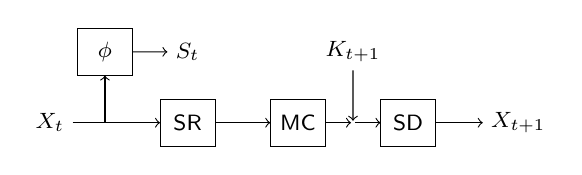
\begin{tikzpicture}[xscale=0.7,yscale=0.6]
      \footnotesize
      % variables
      \draw ( 2, 0) node(Xt){$\fsmState{t}$} ;
      \draw (10.5, 0) node(Xtplus){$\fsmState{t+1}$} ;
      \draw (7.5, 1.5) node(Kt){$K_{t+1}$} ;
      \draw (4.5, 1.5) node(St){$S_t$};
      % operations
      \draw (2.5, 1) rectangle (3.5, 2) node[pos=0.5]{$\filter$} ;
      \draw ( 4, -0.5) rectangle (5, 0.5) node[pos=0.5]{$\shiftR$} ;
      \draw ( 6, -0.5) rectangle (7, 0.5) node[pos=0.5]{$\mixC$} ;
      \draw ( 7.5, 0) node(add)[inner sep=0pt]{$\boxplus$} ;
      \draw (8, -0.5) rectangle (9, 0.5) node[pos=0.5]{$\subW$} ;
      % arrows
      \draw[->] (Xt) -- (4, 0) ;
      \draw[->] (3, 0) -- (3, 1) ;
      \draw[->] (3.5, 1.5) -- (St) ;
      \draw[->] (5, 0) -- (6, 0) ;
      \draw[->] (7, 0) -- (add) ;
      \draw[->] (Kt) -- (add) ;
      \draw[->] (add) -- (8, 0) ;
      \draw[->] (9, 0) -- (Xtplus) ;
    \end{tikzpicture}
    \caption{\label{fig:notations}Notation throughout clocks.}
  \end{subfigure}
  \hfill
  \begin{subfigure}[t]{0.34\textwidth}
    \centering
    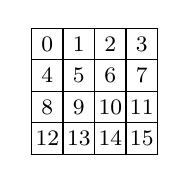
\begin{tikzpicture}[xscale=0.4,yscale=0.4]
      \footnotesize
      \foreach \i in {0,1,2,3}{
        \foreach \j in {0,1,2,3}{
          \draw (\i,\j) rectangle (\i+1,\j+1) ;
        }
      }
      \draw (.5,3.5) node {$0$};
      \draw (1.5,3.5) node {$1$};
      \draw (2.5,3.5) node {$2$};
      \draw (3.5,3.5) node {$3$};

      \draw (.5,2.5) node {$4$};
      \draw (1.5,2.5) node {$5$};
      \draw (2.5,2.5) node {$6$};
      \draw (3.5,2.5) node {$7$};

      \draw (.5,1.5) node {$8$};
      \draw (1.5,1.5) node {$9$};
      \draw (2.5,1.5) node {$10$};
      \draw (3.5,1.5) node {$11$};

      \draw (.5,.5) node {$12$};
      \draw (1.5,.5) node {$13$};
      \draw (2.5,.5) node {$14$};
      \draw (3.5,.5) node {$15$};
    \end{tikzpicture}
    \caption{\label{fig:numbering}Numbering in the FSM.}
  \end{subfigure}
  \hfill~
  
  \caption{\label{fig:notations-all}Our notations. Note that the numbering of the digits differs from the one traditionally used for the \gls{AES}.}
\end{figure}


% Leo: ce qui suit est pour qu'emacs compile bien l'article, pas touche !
%%% Local Variables:
%%% mode: latex
%%% ispell-local-dictionary: "english"
%%% TeX-master: "../main"
%%% End:







\paragraph{S-box Layer ($\subW$).}
We let $\thesbox$ be defined by its lookup table:
\begin{equation}
  \label{eq:thesbox}
  \thesbox = {\tt [1, 12, 6, 11, 14, 3, 15, 5, 10, 9, 13, 16, 7, 8, 0, 2, 4]}
\end{equation}
so that $\thesbox(0) = 1$, $\thesbox(1) = 12$, and so on. It has the following polynomial representation, and is thus of maximum degree: %\jb{il y a un $13x^{10}$  dans le polynome. C'est un $13x^{10}$ ?}\lp{oui}
\begin{equation*}
  \begin{split}
    \thesbox(x) ~=~& 1 + 4 x^{1} + 13 x^{2} + 7 x^{3} + 16 x^{4} + 15 x^{5} + 5 x^{7} + 5 x^{8} \\
    & + 11 x^{9} + 13 x^{10} + 12 x^{11} + 13 x^{12} + 15 x^{14} + x^{15}~.
  \end{split}
\end{equation*}
It was chosen by enumerating all APN permutations of $\mathbb{F}_{17}$, i.e., all permutations $A$ such that the equation $A(x+a)=A(x)+b$ has at most 2 solutions $x$ for all $a \neq 0$ and all $b$. Then, we selected $\thesbox$ among those that offer a good balance between minimizing the number of pairs $(a,b)$ for which the previous equation has exactly two solutions, and minimizing the maximum modulus of the Walsh spectrum (see Definition~\ref{def:fourier}).


\paragraph{Linear Layer ($\mixC$).} We opted for a $4 \times 4$ Maximum Distance Separable (MDS) matrix to ensure optimal diffusion. The matrix we chose is 
\begin{equation}
  \label{eq:mixmat}
  \mixmat = \left[ { \tiny
      \begin{array}{rrrr}
        2 & 1 & 1 & 1 \\
        1 & -1 &1 & -2 \\
        1 & 1 & -2 &-1 \\
        1 & -2 &-1 &1 \\
      \end{array}
    }\right]~.
   % \begin{array}{cccc}
    %  -1 & -1 & -1 & 2 \\
     % -1 & 1 & 2 & -1 \\
     % -1 & 2 & 1 & 1 \\
     % 2 & 1 & -1 & 1 \\
   % \end{array} \right]~.
\end{equation}
%We obtained it by performing an exhaustive search of all $4 \times 4$ matrices with coefficients in ${-2,-1,1,2}$ with at most one coefficient 2 or -2 in each row, and then picking one with the smallest $\ell_2$-norm for a matrix with coefficients in $\mathbb{F}_{17}$. The idea with our initial restrictions to ensure that the $\ell_2$ norm will be low as it depends on the absolute value of the coefficients.

We verified that there is no MDS matrix in  $\mathbb{F}_{17}$ with coefficients in $\{-1,1\}$ by exhaustively  testing all such matrices. As we were interested in MDS matrices with minimal $\ell_2$-norm and we were able to find during the initial experiments  matrices with a squared $\ell_2$-norm of 7, it was evident from the definition of the $\ell_2$-norm that matrices with minimal $\ell_2$-norm could not have coefficients $x$ with $|x| > 2$.  Thus, by testing all matrices with coefficients in $\{-2,-1,1,2\}$, we found a total of $30\>720$ MDS matrices with an $\ell_2$-norm of 7. We selected $\mixmat$ for its symmetries, particularly because it is its own transpose. % Among them, some matrices had a more structured form, as they could be written as 

% \begin{equation*}
%   \mixmat = \left[
%   \begin{array}{rr}
%     A & B  \\
%     B & -A 
%   \end{array} \right]~.
% \end{equation*}
% where both $A$ and $B$ are $2\times 2$ matrices. There were in total 256 matrices of this particular form and we chose $M$ randomly among them, taking into account also that $\mixmat = \mixmat^{T}$.
% (which means its linear behaviour is close to its differential behaviour). \leo{À vérifier}\ac{Cette phrase est bizarre : les branch nb et la distribution des poids sont les memes pour les deux codes si le code est MDS. Donc je ne vois pas ce que cela apporte qu'ils soient identiques.} \leo{ok, j'ai viré}


\paragraph{Filter.} The filter function $\filter$ maps $\mainField^{16}$ (i.e., the full FSM state) to a tuple $(a,b,c,d)$ in $\mainField^{4}$. As summarized in Figure~\ref{fig:filter}, we have that $a,b,c$ and $d$ correspond to the digits of the FSM state with indices 4, 6, 12, and 14 respectively (using the numbering from Figure~\ref{fig:numbering}).


\paragraph{LFSRs.} The whitening LFSR $\whitening$ and the key schedule LFSR $\pseudoKS$ are simply LFSRs over \(\F_p\) of maximum period, and have length 32 and 64 respectively. We obtain a
  maximum-period LFSR over $\mainField^w$ using the coefficients of a
  primitive polynomial as the taps.  More precisely, we used the {\tt SageMath}
  implementation of the finite field $\F_{p^w}$, which resulted in a pseudo-Conway polynomial. The output of the LFSR is taken from its last cell.

  More precisely, an LFSRs of length $\ell$ at time $t$ is a list of digits ${x^t_0, ..., x^t_{\ell-1}}$
  that is clocked as follows:
  \begin{enumerate}
  \item $x_0^{t+1} \gets - \sum_{i=0}^{\ell-1} x_i^t c_i$,
  \item $x_{i}^{t+1} \gets x_{i-1}^t$ for $0 < i < \ell$,
  \item the output is $x_{\ell-1}^t$,
  \end{enumerate}
  where $C=(c_i)_{0 \leq i < \ell}$ is the list of its taps, each being
  a digit of $\mathbb{F}_{17}$. We define $\clock{C}$ to be the function
  applying the operations above to a list ${x^t_0, ..., x^t_{\ell-1}}$
  to update it, and returning $x_{\ell-1}^t$.

  For the key schedule $\pseudoKS$, we use the following taps:
  \begin{equation*}
    \footnotesize
    \begin{split}
      C(\pseudoKS) ~=~& \{9, 4, 6, 4, 8, 6, 6, 16, 3,
                        9, 15, 12, 8, 12, 11, 4, 4, 8, 1,
                        8, 8, 9, 4, 6, 6, 7, 6, 3, \\
                      & 16, 14, 14, 6, 10, 15, 14, 13, 10, 1, 1,
                        10, 13, 11, 14, 10, 7, 4, 15, 8, 16,
                        3, 13, \\
                      & 14, 15, 16, 3, 16, 9, 3, 6,
                        12, 15, 9, 12, 3\}~,
    \end{split}
  \end{equation*}
  and for the whitening LFSR $\whitening$ we use
  \begin{equation*}
    \footnotesize
    \begin{split}
      C(\whitening) ~=~& \{8, 14, 14, 14, 1, 6, 12, 10, 14, 14,
                         14, 5, 2, 5, 6, 13, 6, 15, 14, 3, \\
                       & 13, 16, 1, 13, 9, 1, 7, 15, 13, 6,
                         14, 3\}~.
    \end{split}
  \end{equation*}


\paragraph{Master Key Processing.}
We generate the digits in $\pseudoKS$ first, and then those in $\whitening$. To generate them, we concatenate the 128-bit long master key with an IV and then a byte set to 1. The result is fed into \textsf{SHAKE128}, and the output byte stream of this primitive is used to generate digits of $\mathbb{F}_{17}$ using rejection sampling: if a byte $x$ is equal to 255, we discard it; otherwise, we generate the digit $\lfloor x / 15 \rfloor$. Since $15 \times 17 = 255$, this results in an unbiased transformation.


% Leo: ce qui suit est pour qu'emacs compile bien l'article, pas touche !
%%% Local Variables:
%%% mode: latex
%%% ispell-local-dictionary: "english"
%%% TeX-master: "main"
%%% End:





\subsection{Controlling the Noise Evolution}% in the Homomorphic Evaluation}
\label{sec:rationale-controllin-noise}

We first detail the implementation of each building block of the scheme using \gls{TFHE}, as this is essential to justify our design choices and to understand the evolution of the noise throughout the cipher. We then use this discussion to explain how the noise influences the overall security and efficiency of \coolName.

\paragraph{LFSR.} A naive approach for implementing an LFSR  homomorphically would be to maintain an encrypted state, and update it by computing a linear combination with the feedback coefficients. However, this method would cause the noise in the state to accumulate over time, necessitating periodic use of \gls{PBS} operations to refresh and control the noise growth. For this reason we introduce the principle of the \emph{silent LFSR}. Every output of an LFSR is a linear combination of the digits in its initial state. By computing on the fly the coefficients of these linear combinations in clear, we can evaluate the output of the LFSR at every clock cycle without updating an encrypted version of the internal state. This way, the noise variance in the output of the silent LFSR remains stable over time. This principle is comparable to the approach of {\tt FLIP}~\cite{EC:MJSC16} and follow-up works, whereby a key state is queried without being updated. 

To bound the noise variance in the output of the silent LFSR, we consider the worst-case scenario in which all the coefficients in the linear combinations are of maximal absolute value, i.e., $\frac{p-1}{2}$.\footnote{Constant coefficients of $\mainField$ are encoded as integers of the interval $[-\frac{p-1}{2}, \frac{p-1}{2}]$ to minimize their absolute value and hence their impact on the noise.} The resulting noise variance is thus equal to the original noise variance multiplied by the worst-case squared $\ell_2$-norm. Specifically, in the output of the key schedule LFSR $\pseudoKS$ and of the whitening LFSR $\whitening$, the noise variances $\sigma_\pseudoKS^2$ and $\sigma_\whitening^2$ satisfy
\begin{equation}
  \sigma_\pseudoKS^2 \leq | \pseudoKS | \cdot \left(\frac{p-1}2\right)^2 \cdot \sigma_{\text{fresh}}^2 ~~~\text{and}~~~ \sigma_\whitening^2 \leq | \whitening | \cdot \left(\frac{p-1}2\right)^2 \cdot \sigma_{\text{fresh}}^2,
\end{equation}
where $\sigma_{\text{fresh}}^2$ is the noise variance of the encrypted key material in the LFSRs.

\paragraph{SubDigits.} Each digit of the state of the FSM goes through a \gls{PBS} that evaluates the permutation $\thesbox$. All PBSs can be evaluated in parallel for higher speed. We denote by $\sigma_{\text{\gls{PBS}}}^2$ the noise variance at the output of $\subWords$ for encrypted digits.


\paragraph{ShiftRows.} Since each digit in the state is encrypted in a separate ciphertext digit, this step involves simply rearranging the ciphertext digits within the state. Consequently, it incurs no additional noise growth and no performance impact.

\paragraph{MixColumns.} This operation involves a straightforward linear combination of the digits of the state. The matrix $\mixmat$ has been specifically constructed to minimize the $\ell_2$-norm, considering coefficients in $\F_{17}$. %, while also ensuring optimal diffusion.
From the homomorphic perspective, this choice is crucial, as the variance of the noise increases proportionally with the square of this $\ell_2$-norm, that we denote $L_{\mixC}$. Namely, the noise variance $\sigma^2_\mixC$ after  $\mixColumns$ satisfies $\sigma^2_\mixC = L_{\mixC }^2 \cdot \sigma_{\text{\gls{PBS}}}^2.$


\paragraph{Sums.} The output of $\mixColumns$ is then added to the next output of the LFSR to be injected again into $\subWords$. The noise variance after the addition step corresponds to the sum of both noise variances. Similarly, the noise variance at the output of the scheme, referred to as $\sigma^2_{\text{out}}$, is equal to the sum $\sigma_\whitening^2 + \sigma_{\text{\gls{PBS}}}^2$.
%\medskip


%!TeX root = ../../../thesis.tex
\def\yPseudoKS{-3}

\begin{figure}[t!]
  \centering
    \footnotesize
    \begin{tikzpicture} [xscale=1,yscale=0.45]
      % LFSR interactions
      \draw (-1, \yPseudoKS) rectangle ++(3, 1) node[pos=0.5]{$\pseudoKS$ {\tiny \emph{(Key Schedule)}}} ;
      \draw (-1, 2.5) rectangle (2, 3.5) node[pos=0.5]{$\whitening$ {\tiny \emph{(whitening LFSR)}}} ;
      \draw (3.5, \yPseudoKS + 0.5) node[inner sep=0pt](addm){$\boxplus$} ;

      \node at (0.5, \yPseudoKS - 1) {$\sigma_{\text{fresh}}^{2}$};
      \node at (0.5, \yPseudoKS - 2.5) {\scalebox{0.5}{\verticalgauge{10}}};
      \node at (0.5, 2) {$\sigma_{\text{fresh}}^{2}$};
      \node at (0.5, 0.5) {\scalebox{0.5}{\verticalgauge{10}}};

      \draw (2.7, \yPseudoKS) node[inner sep=0pt](varKS){$\sigma_\pseudoKS^2$} ;
      \node at ($(varKS.south) + (0, -1)$) {\scalebox{0.5}{\verticalgauge{30}}};
      
      \draw (4.5, 3.5) node[inner sep=0pt](varW){$\sigma_\whitening^2$} ;
      \node at ($(varW.north) + (0, 1)$) {\scalebox{0.5}{\verticalgauge{30}}};
      \draw (7, \yPseudoKS) node[inner sep=0pt](varPBS){$\sigma_{\text{\gls{PBS}}}^2$} ;
       \node at ($(varPBS.south) + (0, -1)$) {\scalebox{0.5}{\verticalgauge{50}}};
      \draw (9.7,\yPseudoKS) node[inner sep=0pt](varSR){$\sigma_{\text{\gls{PBS}}}^2$} ;
      \node at ($(varSR.south) + (0, -1)$) {\scalebox{0.5}{\verticalgauge{50}}};
      \draw (8, 2 * \yPseudoKS - 1) node[inner sep=0pt](varMC){$\sigma^2_\mixC$} ;
      \node at ($(varMC.south) + (0, -1)$) {\scalebox{0.5}{\verticalgauge{70}}};
      \draw (4.35, \yPseudoKS + 1.5) node(sum) {$\sigma_\pseudoKS^2+\sigma^2_\mixC$};
      \node at ($(sum.south) + (0, 2)$) {\scalebox{0.5}{\verticalgauge{70}}};
      \draw (9, 3.5) node[inner sep=0pt](varout){$\sigma^2_{\text{out}}  = \sigma_\whitening^2 + \sigma_{\text{\gls{PBS}}}^2$} ;
      \node at ($(varout.north) + (0, 1)$) {\scalebox{0.5}{\verticalgauge{50}}};

      \draw[->] (2, \yPseudoKS + 0.5) -- (addm) ;
      \draw[->] (2.5, \yPseudoKS + 0.5) -- (2.5, \yPseudoKS + 1.5) -- (0.5, \yPseudoKS + 1.5) -- (0.5, \yPseudoKS + 1) ;
      \draw[->] (2.5, 3) -- (2.5, 4) -- (0.5, 4) -- (0.5, 3.5) ;
      % FSM
      \draw[color=blue,style=dashed] (5, \yPseudoKS) rectangle ++(1, 1) node[pos=0.5]{$\subW$} ;
      \draw (8, \yPseudoKS) rectangle ++(1, 1) node[pos=0.5]{$\shiftR$} ;
      \draw (10.3, \yPseudoKS) rectangle ++(1, 1) node[pos=0.5]{$\mixC$} ;
      \draw[->] (addm) -- (5, \yPseudoKS + 0.5) ;
      \draw[->] (6, \yPseudoKS + 0.5) -- (8, \yPseudoKS + 0.5) ;
      \draw[->] (9, \yPseudoKS + 0.5) -- (10.3, \yPseudoKS + 0.5) ;
      \draw[->] (11.3, \yPseudoKS + 0.5) -- (11.6, \yPseudoKS + 0.5) -- (11.6, 2 * \yPseudoKS - 0.5) --  (3.5, 2 * \yPseudoKS - 0.5) -- (addm) ;
      % extracting
      \draw (6.5, \yPseudoKS + 3) rectangle ++(1, 1) node[pos=0.5]{$\filter$} ;
      \draw (7, 3) node[inner sep=0pt](addr){$\boxplus$};
      \draw(11.3, 3) node(s){$Z_i$} ;
      \draw[->] (2, 3) -- (addr) ;
      \draw[->] (7, \yPseudoKS + 0.5) -- (7, \yPseudoKS + 3) ;
      \draw[->] (7, \yPseudoKS + 4) -- (addr) ;
      \draw[->] (addr) -- (s) ;
      % wire width
      % \draw (4.45, -0.2) -- (4.55, 0.2) ;
      % \draw (4.5, -0.5) node{$m$} ;
      % \draw[color=lightgray] (4.45, 2.8) -- (4.55, 3.2) ;
      % \draw[color=lightgray] (4.5, 3.5) node{$r$} ;
    \end{tikzpicture}
    \caption{Evolution of the noise variance in a homomorphic evaluation of \coolName. Operations involving PBSs are in blue and dashed. The gauges allow to visualize the evolution of the noise on a logarithmic scale).}
    \label{fig:noise}
\end{figure}







Figure~\ref{fig:noise} illustrates the evolution of the noise variance throughout the operations of \coolName.
Building on the previous equations, the main constraints influencing the design of \coolName are related to the noise variance at both the input of the \gls{PBS} and the output of the scheme. Specifically, the noise variance $\sigma_\pseudoKS^2+\sigma^2_\mixC$ at the input of the \gls{PBS} (i.e., at input of $\subWords$) must remain sufficiently low, otherwise it could lead to a high probability of \gls{PBS} failure. Additionally, the noise variance $\sigma^2_{\text{out}}  = \sigma_\whitening^2 + \sigma_{\text{\gls{PBS}}}^2$ at the output stream must remain low enough for subsequent applications, ideally as close as possible to the nominal noise variance at the \gls{PBS} output $\sigma_{\text{\gls{PBS}}}^2$. In practical settings, we have $\sigma_{\text{\gls{PBS}}}^2 \gg \sigma_{\text{fresh}}^2$, the noise variances from both LFSRs are negligible compared to $\sigma_{\text{\gls{PBS}}}^2$. For example in our implementation, the noise magnitude of $\sigma_{\text{fresh}}$ is around $2^{14}$, while the noise magnitude of $\sigma_{\text{\gls{PBS}}}$ is around $2^{52}$. Consequently, $\sigma^2_{\text{out}} \approx \sigma_{\text{\gls{PBS}}}^2$ which validates the second constraint. Similarly, the noise variance at the input of the \gls{PBS} is close to that at the output of $\mixColumns$. The latter additionally remains low due to the minimized $\ell_2$-norm of the coefficients of the MDS matrix $\mixmat$, thereby validating the first constraint.


To wrap up, the design of \coolName{} allows to control the evolution of the noise in the FSM while getting a very low number of \gls{PBS} per element. To complete our noise analysis, we need to set the parameters of the \gls{TFHE} scheme to ensure the correctness of the \gls{PBS}. Concretely, the noise \( \sigma_\pseudoKS^2 + \sigma^2_\mixC \) at the input of \( \subWords \) should be low enough to fail with a negligible probability. Of course, these parameters must ensure that the \gls{PBS} operates as fast as possible while maintaining the security of the scheme. In Section~\ref{sec:tfhe-parameters}, we detail our method for selecting the parameters.





% Leo: ce qui suit est pour qu'emacs compile bien l'article, pas touche !
%%% Local Variables:
%%% mode: latex
%%% ispell-local-dictionary: "english"
%%% TeX-master: "main"
%%% End:




% !TeX root = ../../thesis.tex

\section{A Brief Summary of the Security Analysis}
\label{sec:security}

\coolName's full paper provides an extensive analysis of the security of the cipher. Even if these considerations are far from the topic of this manuscript, we provide in this section a brief overview of this analysis. We refer to the full paper \cite{transistor} for the developments of the proofs.


\paragraph{Time-Memory-Data Trade-Offs}

To dimension the size of the LSFR, we computed a bound to ensure that exhaustive attacks are out of reach even when leveraging trade offs with pre-computation and storage. 

Using $\pseudoKS = 64$ and $\whitening = 32$, the length of the keystream generated from the same key is limited to $2^{31}$ digits. As a result, TMDTO attacks have a time complexity of $2^{296}$ in the single IV-setting, which drops to $2^{130}$ when keystreams generated from $2^{130}$ IVs are available to the attacker.

\paragraph{Guess and Determine}

In this kind of attacks, the attacker links the FSM state $\fsmState{t}$ to the filter output $S_t$ and try to guess the key schedule $K_t$.

Based on an analysis of the filtering procedure of \coolName, we showed that in total the attacker has to guess $\frac{12}{16}|\pseudoKS|$ digits, leading to a complexity \( p^{\frac{3}{4} | \pseudoKS |} \approx 2^{196}\) without taking into account the whitening LFSR. If we consider it, the attacker first has to
guess its content, leading to an attack with complexity
\( p^{\frac{3}{4} | \pseudoKS | + | \whitening |} \approx 2^{294}\).
%


\paragraph{Three consecutive outputs are statistically independent of the secret key}

The basic strategy in (fast) correlation attacks against stream ciphers consists in recovering some information about (a part of) the initial state of the cipher from the knowledge of the keystream. 
In this context, an important quantity is the smallest length of output sequence $(S_t)_{t\in \N}$ that can provide information on the sequence produced by the key-LFSR. In the paper we prove that this length is 4, that is to say 3 consecutive outputs are statistically independent of the secret key. This is a very good performance with respect to the state of the art: the only other cipher with this property is \texttt{Rocca} \cite[Section 4.5]{ToSC:SLNKI21}. However, in this case this property has been derived from an automatic search method, while the structure of \coolName enables us to derive this argument in a very simple way from the MDS property of~$\mixColumns$. 


\paragraph{(Fast) Correlation Attacks Using Biased Linear Relations}


Our paper also provides an estimation of the minimal data complexity required to recover the internal state of the key-register from the knowledge of the output sequence $(S_t)_{t\in \N}$, given that at least four consecutive outputs $(S_t, S_{t+1}, S_{t+2}, S_{t+3})$ need to be considered together. Applying the so-called Xiao-Massey lemma \cite{add:XiaMas88,add:Bry89}, it is possible to see that as soon as the key-LFSR and the considered segment of the output sequence are not statistically independent, there exists a biased linear relation between the digits of these two sequences.

In the paper, we exhibit an upper bound on the correlation of such linear relation. This bound depends on the minimal number of active S-boxes over $n$ rounds, as well as the modulus of the Fourier coefficients of \coolName's S-box. We show that the design of our S-box brings the correlation down to a value small enough so that the amount of keystream that the attacker has to observe exceed the limit of $2^{31}$ digits fixed by TMDTO trade-offs.


\paragraph{Linear Distinguishers}

Another type of attack studied in the paper is linear distinguishing attacks \cite{EC:MeiSta88,EC:CanTra00,FSE:CheJohSme00,C:TIMAZ18}. These attacks do not recover the initial state of the key-register, but the counterpart is that they can use together several keystream segments produced from multiple initial state. They consist in exhibiting a biased linear relation among the keystream digits. Such a relation is typically derived from a \textit{parity-check equation} for the key-LFSR, defined by the multiples of the LFSR feedback polynomial. 

In \coolName's design, this polynomial has been chosen so that it shows good properties regarding the utility of these parity-check equations. The conclusion of our analysis is that such an attack would be more expensive than an exhaustive search for the key .


\medskip

The full security analysis also takes into account algebraic attacks; such that Gröbner basis or the use of annihilators of the filtering function.



\section{Performances of Transciphering with \coolName}
\label{sec:bench}


This section focuses on the performances of transciphering with \coolName. We first address the wrapping of a (\coolName) symmetric key as a compact set of \gls{TFHE} ciphertexts for which we additionally introduce a trade-off between bandwidth and computation. Next, we explain how to manage different data representations to be able to fit with the input format of the server application. We then provide a detailed description of the homomorphic evaluation of \coolName. We finally give some implementation benchmarks and comparison to the state of the art.

\subsection{Key Wrapping and Bandwidth in \gls{TFHE} Transciphering} \label{sec:key_wrapping}

Assume one wants to generate a fresh \gls{TFHE} ciphertext vector $(c_1, \ldots, c_t)$ for a plaintext vector $(m_1, \ldots, m_t) \in \mathbb{Z}_p^t$, where $c_i = (a_{i,1}, \ldots, a_{i,n}, b_i)$, for every $i \in [1,t]$. Since the $a_{i,j}$'s are uniformly sampled at random over $\mathbb{Z}_q$, a folklore trick is to generate them pseudorandomly from a seed. We get the following compressed encryption procedure (where $\lambda$ denotes the security level in bits):
  
\begin{center}
\noindent\framebox{
\begin{minipage}{0.8\textwidth}
\underline{$\mathtt{CompressEncrypt}(s,m_1, \ldots, m_t)$}
	\vspace{-2mm}
	\begin{enumerate}
	\item Sample $\mathsf{seed} \gets \{0,1\}^\lambda$
	\smallskip
	\item Expand $((a_{i,j})_{1 \leq j \leq n})_{1 \leq i \leq t} \gets \mathsf{PRG}(\mathsf{seed})$
	\smallskip
	\item $\forall \:i \in [1,t]$: $b_i \gets \sum_{j=1}^n a_{i,j} \cdot s_j + \tilde{m}_i + e_i$ with $e_i \gets \chi_{\sigma}$
	\smallskip
	\item Return $(\mathsf{seed}, b_1, \ldots, b_t)$
\end{enumerate}
\end{minipage}}
\end{center}

\smallskip

Recovering standard \gls{TFHE} ciphertexts $c_1$, \ldots, $c_t$ from the compressed form $(\mathsf{seed}, b_1, \ldots, b_t)$ is simply done by expanding the $a_{i,j}$'s from $\mathsf{seed}$. The size of the obtained compressed ciphertext vector is $\lambda + t \cdot \log_2(q)$ against $t \cdot (n+1) \cdot \log_2(q)$ for a standard \gls{TFHE} encryption, meaning a compression by a factor about $(n+1)$. 

This compressed \gls{TFHE} encryption method can be applied directly to transmit homomorphically encrypted data from the user to the server. Alternatively, it can be combined with transciphering to encrypt a symmetric key. The resulting bandwidth requirements and the corresponding plaintext-to-ciphertext expansion factor are summarized in Table~\ref{tab:formulas_bandwidth}, where they are further compared with the naive (uncompressed) \gls{TFHE} encryption. In particular, for \coolName, a wrapped key is of size $\lambda + (|\mathcal K| + |\mathcal W|) \cdot \log_2(q)$, (which in our case gives 784 bytes) for a security of $\lambda = 128$ bits (target security of \coolName), the standard choice of $q= 2^{64}$ (which we use in our implementation) and $|\mathcal K| + |\mathcal W| = 96$ per the specification of \coolName (see Section~\ref{sec:description}). This fixed cost is hence very quickly amortized while the amount of data to encrypt grows.
Moreover, this approach can be applied to the server keys as well, which are actually encryptions of the secret key's bits. We took this optimization into account in our estimations of the server key sizes in Table \ref{tab:server_key_size}. 

\paragraph{Compressing further.}

We introduce hereafter a tweak to compress a \gls{TFHE} encryption further than the folklore compression. By definition of the \gls{TFHE} encryption process, the least significant bits of the body $b_i = \sum_{j=1}^n a_{i,j} \cdot s_j + \tilde{m}_i + e_i$ are randomized by the error $e_i$ and can hence be discarded without loss of information. We can thus tweak the above compressed encryption process by returning $(\mathsf{seed}, \mathrm{Tr}_\ell(b_1), \ldots, \mathrm{Tr}_\ell(b_t))$ where $\mathrm{Tr}_\ell(\cdot)$ denotes the truncation of the $\ell$ least significant bits. To decompress such ciphertexts, besides pseudorandomly generating the masks from the seed, one just needs to pad the truncated bodies with $\ell$ bits to $0$. By the randomness of the mask, the effect of this truncation plus $0$-padding is to add a uniform random error of $\ell$ bits to the body, namely an error of standard deviation: 
$$\sigma_0^2  = \frac{(2^\ell - 1)^2}{12} \approx \frac{2^{2\ell}}{12} \approx 0.08 \cdot 2^{2\ell} ~.$$

\noindent This optimization comes in two flavors:
\begin{enumerate}
	\item \emph{The ``free'' variant.} The number of truncated bits $\ell$ is selected to have a small impact on the noise distribution. For instance in \coolName, the noise of the fresh ciphertexts is summed with the noise coming from the FSM. Thus, we can compute $\ell$ to keep $\sigma^2_{\mathcal W} < \sigma^2_{\text{\gls{PBS}}}$. Our experiments shows $\sigma^2_{\text{\gls{PBS}}} = 2^{52}$, so running the numbers we find that we can truncate up to $\ell=19$ bits, allowing to reduce the volume of the \gls{TFHE} ciphertexts to send by a factor $1 - \frac{19}{64} \approx 0.7$.
	
	\smallskip
	
	\item \emph{The communication-computation trade-off.} In this variant, one selects a high value of $\ell$. The truncated body should at least contain $\log_2(p)$ bits to keep the plaintext information, plus a margin of a few bits in order to remain bootstrappable. Denoting this margin $\delta$, the truncated body should be of at least $\log_2(p) + \delta$ bits and $\ell$ can be up to $\log_2(q) - (\log_2(p)+\delta)$. Taking the maximum level of truncation, inducing the maximum level of bootstrappable noise, implies some adaptation of the underlying homomorphic computation. Specifically, it should start with applying a noise-reduction bootstrapping to the decompressed ciphertexts before performing the original evaluation. We hence obtain a trade-off with reduced bandwidth against additional bootstrappings.
\end{enumerate}

In the context of transciphering with \coolName, the trade-off provided by the second option gives rise to an initialization procedure which consists in decompressing and bootstrapping the wrapped key. 

This kind of compression has been more extensively studied in the concurrent work \cite{EPRINT:BCCS24}.

\begin{table}[t!]
	\centering
        \caption{Bandwidth of homomorphic ciphertexts (in bits).}
        % The total bandwidth is the fixed cost + $t$ times the cost per message to encrypt $(m_1, \ldots, m_t)\in \mathbb{Z}_p^t$.
	\label{tab:formulas_bandwidth}
        {
          \renewcommand{\arraystretch}{1.1}
          \footnotesize
          \scalebox{0.9}{
            \begin{tabular}{|l|*{3}{>{\centering\arraybackslash}p{3.5cm}|}}
              \hline
              \textbf{Approach used} & \textbf{Naive} & \textbf{Compressed} & \textbf{\coolName} \\
              \hline
              Fixed cost & 0 & $\lambda$ & $\lambda + (|\mathcal{K}|+|\mathcal{W}|) \cdot \log_2(q)$ \\
              \hline
              Per message in $\mathbb{Z}_p$ & $(n+1) \cdot \log_2(q)$ & $\log_2(q)$ & $\log_2(p)$ \\
              \hline
              Expansion factor~ & $(n+1) \cdot {\log_2(q)}/{\log_2(p)}$ & ${\log_2(q)}/{\log_2(p)}$ & 1 \\
              \hline
            \end{tabular}}
        }
	
\end{table}



\subsection{Transciphering vs. Data Representation}
\label{sec:data_representation}

Managing data representation is a common challenge when working with \gls{TFHE}. Since this scheme is only efficient at very low precision, an abstraction layer is required to construct practical data types (e.g., 8-, 32-, or 64-bit integers) from smaller encrypted chunks. Common constructions include radix-based decompositions and Chinese Remainder Theorem (CRT) representations, leading to different efficiency trade-offs. Carry propagation in radix-based representations is notoriously slow due to the large number of required bootstrappings, while CRT representations impose constraints on feasible operations. These constructions have been studied in~\cite{JC:BBBCLO23}. 

As a result, there is no universal representation that is optimal for all homomorphic operations. Thankfully, the representation of data in the transciphering algorithm can be chosen independently of that of the homomorphic application running on the server. If the representation in $\mathbb Z_p$ does not suit the application, the server can convert the ciphertexts to the desired representation before running the application. %Such a conversion can be either applied to the \gls{TFHE} ciphertexts obtained by the server after transciphering, or directly on the keystream (in this case, the symmetric ciphertexts are encoded directly in the desired representation, and the encryption/decryption operation is performed in the corresponding space). In both cases, it simply requires a bootstrapping for each element of $\mathbb Z_p$. 
We stress that this additional step of conversion would be necessary for any transciphering algorithm, as the data format desired in output of transciphering is completely application-dependent.

	
As a concrete example, assume that the data to be encrypted (i.e., the input to the homomorphic computation) consists of elements from $\mathbb{Z}_{16}$. The overall transciphering process unfolds as follows. On the client side, the plaintext is first embedded from $\mathbb{Z}_{16}$ into $\mathbb{Z}_{17}$ before being encrypted using \coolName. On the server side, the keystream is homomorphically generated and then used to homomorphically decrypt the ciphertext. This results in a \gls{TFHE} encryption of the original plaintext, now embedded in $\mathbb{Z}_{17}$, meaning that the plaintext space for the \gls{TFHE} encryption is $\mathbb{Z}_{17}$. A programmable bootstrapping (\gls{PBS}) operation is then applied to switch the plaintext space from $\mathbb{Z}_{17}$ back to $\mathbb{Z}_{16}$.

In terms of computation, this process adds one \gls{PBS} per $\mathbb{Z}_{16}$-element of the original plaintext, in addition to the four \gls{PBS} per element required for keystream generation with \coolName. Moreover, embedding $\mathbb{Z}_{16}$ into $\mathbb{Z}_{17}$ increases the size of the encrypted data by a factor of $1 + 1/16 = 1.0625$.

This approach can be generalized to address other plaintext representations. In particular, for larger chunks of bits, the bootstrapping operation would allow to merge several elements of $\mathbb{Z}_{16}$ (embedded into $\mathbb{Z}_{17}$) into one element of $\mathbb{Z}_{2^\ell}$ with $\ell > 4$. On the other hand, one may split an element of $\mathbb{Z}_{16}$ (or its $\mathbb{Z}_{17}$ embedding) into 4 elements of $\mathbb{Z}_{2}$ using a \gls{PBS} with multiple look-up tables (``PBSmanyLUT'') as proposed in~\cite{AC:CLOT21}.



	
\subsection{Detailed Homomorphic Implementations}
\label{sec:detailed_implementation}

In the following, we provide a more detailed way of how we implemented the homomorphic version of \coolName.

\paragraph{Homomorphic evaluation of LFSRs.}
The \coolName design involves two LFSRs operating on elements of $\F_{17}$. The standard way to implement an LFSR is to evaluate the linear feedback function on the state at each clock cycle, thus producing a new element that enters the state, while the state is shifted to output an element. 

We suggest the \emph{silent LFSR} approach for the homomorphic evaluation of LFSRs. In this approach, the encrypted LFSR state is immutable to avoid any noise growth in the underlying ciphertexts (hence keeping the LFSR ``silent''). We use the fact that every output element of the LFSR can be expressed as a linear combination of the initial state. So, at each clock cycle, we compute \emph{in the clear} the coefficients of this linear combination and homomorphically evaluate it on the immutable encrypted state. This process is depicted in Algorithm~\ref{alg:lsfr}.


\begin{algorithm}[t!]
    \caption{\texttt{LFSR.clock} - Produce a pseudo random element of the state. \label{alg:lsfr}}
    
    \KwIn{
        $\left\{
        \begin{aligned}
            &\ell: \text{ Size of the state of the LFSR.} \\
            &(u_1, \dots, u_\ell): \text{ Encrypted initial state of the LFSR.} \\
            &(\lambda_1^{(0)}, \dots, \lambda_\ell^{(0)}): \text{ Coefficients of retroaction in the definition of the LFSR.} \\
            &(\lambda_1^{(i)}, \dots, \lambda_\ell^{(i)}): \text{ Previous coefficients used in the linear combination.}
        \end{aligned}
        \right.$
    }

    \KwResult{
        $\left\{
        \begin{aligned}
            &o^{(i)}: \text{ Encryption of the $i$-th pseudorandom element of $\F_{17}$.} \\
            &(\lambda_1^{(i+1)}, \dots, \lambda_\ell^{(i+1)}): \text{ Updated coefficients of the linear combination.}
        \end{aligned}
        \right.$
    }

    % Add vertical space and horizontal line
    \vspace{0.5em} % adjust the space as needed
    \hrule
    \vspace{0.5em} % adjust the space as needed

    $o^{(i)} \gets 0$

    \Comment{Evaluation of the linear combination}
    \For{$k \in \{1, \dots, \ell\}$}{
        $o^{(i)} \gets \texttt{SumTFHE}(o^{(i)}, \texttt{ClearMultTFHE}(u_k, \lambda_k^{(i)}))$
    }
    \Comment{Update of the next coefficients}
    \For{$k \in \{2, \dots, \ell\}$}{
        $\lambda_k^{(i+1)} \gets \lambda_{k-1}^{(i)} + \lambda_\ell^{(i)} \cdot \lambda_k^{(0)}$
    }
    $\lambda_1^{(i+1)} \gets \lambda_\ell^{(i)} \cdot \lambda_1^{(0)}$
    
    \Return{$o^{(i)}$}
    
\end{algorithm}




\paragraph{Homomorphic evaluation of} \coolName. The complete homomorphic evaluation of a round of on clock cycle of \coolName is depicted in Algorithm~\ref{alg:transistor}, using $\pseudoKS.\texttt{clock}$ and $\whitening.\texttt{clock}$ as subroutines (i.e., Algorithm~\ref{alg:lsfr} evaluated on the key schedule and whitening LFSRs). The most computation intensive part of the algorithm is by far the evaluation of the \gls{PBS} in $\subWords$ which can be fully parallelized to reduce the latency.


 \begin{algorithm}[t!]
    \caption{\texttt{Transistor.clock} - Produce $r$ encypted elements of the key stream}
    \label{alg:transistor}
    
 
    \KwIn{
        $\left\{
        \begin{aligned}
        	&\mathcal K: \text{the LFSR used for the pseudo-keyschedule and its state (cf Algorithm \ref{alg:lsfr}).}\\
            &\mathcal W: \text{the LFSR used for the whitening.}\\	
            &X = \left ( \begin{array}{ccc}
            x_{1,1} & \dots & x_{1,\sqrt{m}}\\
            \dots & \dots & \dots\\
            x_{\sqrt{m},1} & \dots & x_{\sqrt{m},\sqrt{m}}\\
            \end{array} \right ): \text{ Encrypted state of the FSM} \\
        \end{aligned}
        \right.$
    }

    \KwResult{
        $\left\{
        \begin{aligned}
            &Y = (y_1, \dots, y_r): \text{ Encryption of $r$ elements of the  key stream } \\
        \end{aligned}
        \right.$
    }

    % Add vertical space and horizontal line
    \vspace{0.5em} % adjust the space as needed
    \hrule
    \vspace{0.5em} % adjust the space as needed

    \Comment{Compute the pseudo-key schedule and adds it to the FSM}
    \For{$i \in [1, \sqrt m]$}{
        \For{$j \in [1, \sqrt m]$}{
            $k_{i,j} \gets \pseudoKS.\texttt{clock}()$\\
            $x_{i,j} \gets \texttt{SumTFHE}(x_{ij}, k_{i,j})$\\
        }
    }
    \Comment{Compute $\subWords$ with a layer of PBS}
    \For{$i \in [1, \sqrt m]$}{
        \For{$j \in [1, \sqrt m]$}{        
            $x_{i,j} \gets \texttt{PBS\_TFHE}(x_{i,j}, S)$\\
        }
    }
    \Comment{Extract the output bits and whiten them}
    $(y_1, \dots, y_r) \gets \phi(X)$\\
    \For{$i \in [1, r]$}{
        $w_i \gets \whitening.\texttt{clock}()$\\
        $y_i \gets \texttt{SumTFHE}(y_i, w_i)$\\
    }
    \Comment{Compute $\shiftRows$, (same as in clear)}
    $X \gets \shiftR(X)$

    \Comment{Compute MixColumns}
    \For{$i \in [1, \sqrt m]$}{
        \For{$j \in [1, \sqrt m]$}{
            $z_{i, j} \gets 0$\\
            \For{$k \in [1, \sqrt m]$}{
                $z_{i, j} \gets \texttt{SumTFHE}(z_{i, j}, \texttt{ClearMultTFHE}(x_{k, j}, MC_{i, k}))$\\
            }
        }
    }

    \Return{$Y$}

\end{algorithm}






\subsection{\gls{TFHE} Parameters} 
\label{sec:tfhe-parameters}


We discuss hereafter the selection of the different \gls{TFHE} parameters involved in the homomorphic implementation of \coolName. An extensive presentation of the \gls{TFHE} parameters and their role within the scheme can be found in Section \ref{sec:about_problem}.

Figure \ref{fig:structure_fhe} shows the ciphertext format at the different steps of the homomorphic evaluation of \coolName. It shows that the manipulated ciphertexts can be of three different types: LWE ciphertexts of dimension $n_{\text{short}}$, LWE ciphertexts of dimension $n_{\text{long}}$, or GLWE ciphertexts of dimension $k$ and polynomial degree $N$.
	

\begin{figure}[t!]
  \centering
    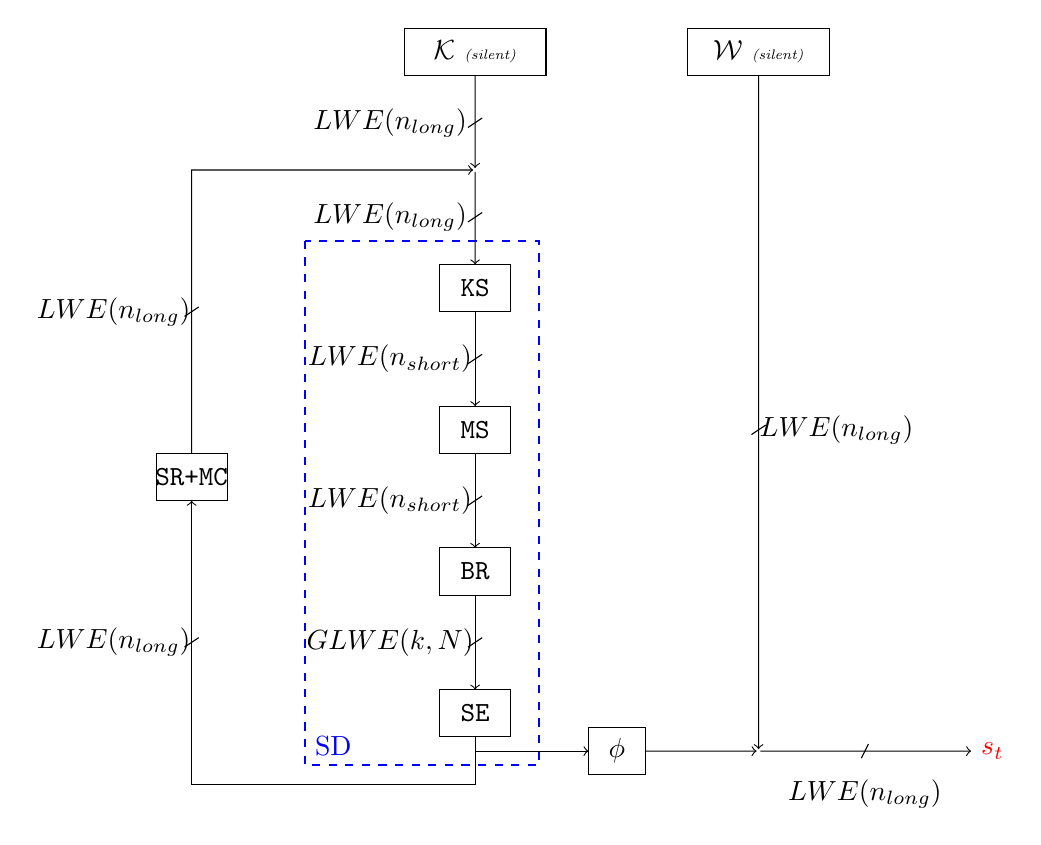
\begin{tikzpicture}[xscale=0.9,yscale=0.6]
 
    %LSFRs
    \draw[] (0, 0) rectangle (2, 1) node[pos=0.5]{$\pseudoKS$ {\tiny \emph{(silent)}}} ;
    \draw[] (4, 0) rectangle (6, 1) node[pos=0.5]{$\whitening$ {\tiny \emph{(silent)}}} ;
    \draw (1, -2) node[inner sep=0pt](addm){$\boxplus$} ;
    \draw[->] (1, 0) -- (addm);

    % FSM
    \draw[] (0.5, -4) rectangle (1.5, -5) node[pos=0.5,color=black](ks){$\texttt{KS}$} ;
    \draw[] (0.5, -7) rectangle (1.5, -8) node[pos=0.5,color=black](ms){$\texttt{MS}$} ;
    \draw[] (0.5, -10) rectangle (1.5, -11) node[pos=0.5,color=black](br){$\texttt{BR}$} ;
    \draw[] (0.5, -13) rectangle (1.5, -14) node[pos=0.5,color=black](se){$\texttt{SE}$} ;
    \draw[] (-3.5, -8) rectangle (-2.5, -9) node[pos=0.5,color=black](srmc){$\texttt{SR+MC}$} ;

    % Draw dashed blue box for SB
    \draw[dashed, blue, thick] (-1.4, -3.5) rectangle (1.9, -14.6);
    \node[blue] at (-1, -14.2) {SD}; % Label for the box

    % FSM connections
    \draw[->] (addm) -- (1, -4);
    \draw[->] (1, -5) -- (1, -7);
    \draw[->] (1, -8) -- (1, -10);
    \draw[->] (1, -11) -- (1, -13);
    \draw[->] (1,-14) -- (1, -15) -- (-3, -15) -- (-3, -9);
    \draw[->] (-3, -8) -- (-3, -2) -- (addm);

    % Extraction
    \draw (5, -14.3) node[inner sep=0pt](addr){$\boxplus$} ;
    \draw[] (2.6, -13.8) rectangle (3.4, -14.8) node[pos=0.5,color=black]{$\phi$} ;

    \draw[->] (1, -14.3) -- (2.6, -14.3);
    \draw[->] (3.4, -14.3) -- (addr);
    \draw[->] (5, 0) -- (addr);
    \draw[->] (addr) -- (8, -14.3);
    \draw[color=red] (8.3, -14.3) node(s){$s_t$} ;



    % Wire type
    \draw (0.9, -1.1) -- (1.1, -0.9) ;
    \draw (-0.2, -1) node{$LWE(n_{\text{long}})$} ;
    \draw (0.9, -3.1) -- (1.1, -2.9) ;
    \draw (-0.2, -3) node{$LWE(n_{\text{long}})$} ;
    \draw (0.9, -6.1) -- (1.1, -5.9) ;
    \draw (-0.2, -6) node{$LWE(n_{\text{short}})$} ;
    \draw (0.9, -9.1) -- (1.1, -8.9) ;
    \draw (-0.2, -9) node{$LWE(n_{\text{short}})$} ;
    \draw (0.9, -12.1) -- (1.1, -11.9) ;
    \draw (-0.2, -12) node{$GLWE(k, N)$} ;
    \draw (-3.1, -12.1) -- (-2.9, -11.9) ;
    \draw (-4.1, -12) node{$LWE(n_{\text{long}})$} ;
    \draw (-3.1, -5.1) -- (-2.9, -4.9) ;
    \draw (-4.1, -5) node{$LWE(n_{\text{long}})$} ;
    \draw (4.9, -7.6) -- (5.1, -7.4) ;
    \draw (6.1, -7.5) node{$LWE(n_{\text{long}})$} ;
    \draw (6.45, -14.45) -- (6.55, -14.15) ;
    \draw (6.5, -15.2) node{$LWE(n_{\text{long}})$} ;

    \end{tikzpicture}
  \vspace{1em}
  \hfill~
  \caption{\label{fig:structure_fhe} Types and shapes of ciphertexts in homomorphic \coolName. The $\subWords$ is broken down into its elementary components}
\end{figure}


% Leo: ce qui suit est pour qu'emacs compile bien l'article, pas touche !
%%% Local Variables:
%%% mode: latex
%%% ispell-local-dictionary: "english"
%%% TeX-master: "../main"
%%% End:






\paragraph{Optimization of the \gls{TFHE} parameters.}
To generate a set of parameters, we use the method developed in~\cite{JC:BBBCLO23}. Given the negligible noise contribution from the LFSRs, the FSM can be modeled using the \emph{atomic pattern} introduced in~\cite{JC:BBBCLO23} (specifically the instance referred to as $\mathcal{A}^{(\text{CJP21})}$), which is a pattern of homomorphic operators taking a set of ciphertexts in input, computing linear combinations of those ciphertexts and applying a programmable bootstrapping to each of them. The FSM round in \coolName which composes a multiplication by a constant matrix ($\mixColumns$), followed by a bootstrapping step ($\subWords$) is precisely an instance of such an atomic pattern. The framework proposed in~\cite{JC:BBBCLO23} generates parameters that guarantee a specified security level $\lambda$ for the LWE encryption and target error probability $p_{\text{err}}$, while optimizing the \gls{PBS} to be as fast as possible. 

Table \ref{tab:transistor_parameters} shows the parameters used for our experiments, all ensuring 128 bits of security. The obtained security levels $\lambda_{\text{short}}$ et $\lambda_{\text{long}}$ have been estimated using the \texttt{lattice estimator}~\cite{lattice-estimator}.

\begin{table}[t!]
\centering
\caption{\gls{TFHE} Parameters used in our experiments}.
\label{tab:transistor_parameters}
\renewcommand{\arraystretch}{1.3}  % Adjust row spacing
\scalebox{1}{
	\begin{tabular}{|c||*{12}{>{\centering\arraybackslash}p{0.8cm}|}}
		\hline
		$p_{\text{err}}$ & $q$ & $n_{\text{short}}$ & $k$ & $N$ & $\sigma_{\text{short}}$ & $\sigma_{\text{long}}$ & $\baseDecompPBS$ & $\levelDecompPBS$ & $\baseDecompKS$ & $\levelDecompKS$ & $\lambda_{\text{short}}$ & $\lambda_{\text{long}}$\\
		\hline
		$2^{-40}$ & $2^{64}$ & 788 & 2 & 1024 & $2^{47}$ & $2^{14}$ & $2^{23}$ & 1 & $2^4$ & 3 & 131.8 & 128.9\\
		\hline
		$2^{-128}$ & $2^{64}$ & 774 & 1 & 2048 & $2^{47}$ & $2^{14}$ & $2^{23}$ & 1 & $2^3$ & 5 & 131.8 & 128.9\\
		\hline
\end{tabular}
}
	\end{table}



\paragraph{Encryption security.} 
The security level (in bits) of the LWE ciphertexts is a function of the modulus $q$, the dimension $n$ and the noise standard deviation $\sigma$. While no explicit formula exists for this function, the \emph{lattice estimator} tool allows to produce an estimation of this function by simulating the main attacks of the literature~\cite{lattice-estimator}, which we denote $\mathcal{O}$ (for \emph{security oracle}). The selected \gls{TFHE} parameters are constrained to satisfy $\mathcal{O}(q,n,\sigma) \geq \lambda$ for both $(q,n,\sigma) = (q,n_{\text{short}},\sigma_{\text{short}})$ and $(q,n,\sigma) = (q,n_{\text{long}},\sigma_{\text{long}})$.



\paragraph{Correctness of the \gls{PBS}.} To compute the error probability $p_{\text{err}}$, we have to evaluate the variances occurring inside the programmable bootstrapping of the $\subWords$ layer. This reasoning will be more detailed in Chapter \ref{chap:parameters} (with additional bits in Appendix \ref{sec:cjp_details}). Here, we provide a short reasoning sufficient for our purpose.


In the following, we denote the maximum error probability of the bootstrapping by $p_{\text{err}} := 2^{-\kappa}$. We aim to choose parameters such that the \gls{PBS} outputs a correct ciphertext with probability at least $1-p_{\text{err}}$. This translates to the following constraint:
$$\sigma^2_{\text{in-}\textsf{BR}} \leq  C(\kappa) \cdot \left(\frac1{4p}\right)^2 ~~~\text{with}~~~C(\kappa) := \left(\frac{1}{\sqrt{2} \cdot \mathsf{erfc}^{-1}(2^{-\kappa})}\right)^2 ~.$$
Under the Gaussian assumption, the noise in input of the \textsf{BlindRotate} is lower than $\mathsf{erfc}^{-1}(2^{-\kappa}) \cdot \sqrt{\sigma^2_{\text{in-}\textsf{BR}}}$ with probability $1-2^{-\kappa}$. The above constraint thus implies that, with probability $1-2^{-\kappa}$, the noise is lower than $1/{4p}$ which ensures the correctness of the \gls{PBS}. 

As $|\mathcal W| \leq |\mathcal K|$, we can check that we always have $\sigma^2_{\text{out}} \leq \sigma^2_{\text{in-}\textsf{\gls{PBS}}}$ which implies that the output is always bootstrappable with correctness probability at least $1-p_{\text{err}}$ in the subsequent bootstrapping.


\subsection{Performances} \label{sec:performances}

We provide hereafter some benchmarks of our implementation of \coolName for two sets of parameters tailored for two different error probabilities. We first consider $\perr = 2^{-40}$, which is a common choice in the literature to benchmark homomorphic implementations. Our results for this error probability allow a fair comparison with the state of the art. While such an error probability theoretically allows transciphering to be error-free with a large amount of data with good probability, some recent works have shown that non-negligible error probabilities could be exploited by an adversary in some contexts~\cite{C:CSBB24,CCS:CCPSS24}. Thus, we also provide another set of parameters and associated benchmark for $\perr =  2^{-128}$.

Our implementation relies on our customized version of \texttt{tfhe-rs}~\cite{tfhe-rs} which has been adapted to support odd $p$ (size of the plaintext space), that we described in Section \ref{sec:library}. The experiments were carried on a processor 12th Gen Intel(R) Core(TM) i5-1245U with 4.4 GHz. Table \ref{tab:perfs} summarizes the obtained timings for the two sets of parameters. The throughput is computed assuming that $\log_2(17)$ bits are encoded on one element of $\F_{17}$. Encoding 4 bits on each element would scale the throughput by a factor $4/\log_2(17) \approx 0.98$.

\begin{table}[t!]
	\centering
		\caption{Performances of our two instances of \coolName.}
	\label{tab:perfs}
	\renewcommand{\arraystretch}{1.2}  % Adjust row spacing
	\begin{tabular}{|c||*{3}{>{\centering\arraybackslash}p{3cm}|}}
		\hline
		~~$p_{\text{err}}$~~ & Time for one \gls{PBS} & Latency (one round) & Throughput\\
		\hline
		$2^{-40}$ & 11.9 ms & 195 ms & 83.84 bits/s\\
		\hline
		$2^{-128}$ & 15.28 ms & 251 ms & 65.10 bits/s\\
		\hline
	\end{tabular}
\end{table}



Although our current implementation does not leverage the inherent parallelism of \coolName, it is important to note that it can be easily parallelized across 16 threads. Specifically, during the $\subWords$ steps, which dominate the overall runtime, the 16 \gls{PBS} operations can be executed concurrently. This parallelization would result in nearly a 16-fold reduction in total execution time.

Without taking into account the server key\ifeprint(whose sizes are shown in Table \ref{tab:server_key_size})\fi, and using compressed encryption (Section \ref{sec:key_wrapping}),  transciphering 1 KB of plain data requires 1.78 KB of data to be sent, instead of 64 KB. For larger amounts of message, the volume of the encrypted symmetric key becomes negligible with respect to the message: for 1 MB of plain data, we use 1.0008 MB, and for 1 GB, this goes down to 1.000001 GB. The two sets of parameters yield the same bandwidth consumption, but not the same running time as shown in Table \ref{tab:perfs}.



By applying the ``free truncation optimization" introduced in Section \ref{sec:key_wrapping}, we can reduce the volume of the encrypted symmetric key by a factor~0.7. This is particularly useful when transciphering a small volume of data (the volume of the encrypted key being preponderant). For example, to transcipher 1 KB of data, using this technique decreases the volume from 1.78~KB to 1.54~KB. 

In Table \ref{tab:server_key_size} we provide the sizes for the server keys, namely the \emph{key-switching key} ($\KSK$) and the \emph{bootstrapping key} ($\BSK$) while using the ciphertext compression technique described in Section~\ref{sec:key_wrapping}. Those keys are only generated and communicated to the server once (during some user enrollment step).

\begin{table}[t!]
  \centering
  \caption{Size of the server keys for the two considered sets of parameters. 
    % This is agnostic to the volume of message sent. 
    \label{tab:server_key_size}}
  
  \renewcommand{\arraystretch}{1.2}  % Adjust row spacing
  \scalebox{0.9}{
    \begin{tabular}{|c||*{3}{>{\centering\arraybackslash}p{4cm}|}}
      \hline
      & Theoretical sizes & Sizes for $p_{\text{err}} = 2^{-40}$ & Sizes for $p_{\text{err}} = 2^{-128}$ \\
      \hline
      ~KSK~ &  $n_{\text{long}}\cdot l_{\text{KS}} \cdot \log_2 q $ & 49 KB & 82 KB  \\
      \hline
      ~BSK~ &  $n_{\text{short}} \cdot l_{\text{BS}} \cdot \log_2 q \cdot N \cdot (k+1)$ & 6.5 MB & 12.7 MB  \\
      \hline
    \end{tabular}
}
\end{table}




\subsection{Comparisons to the State of the Art}
\label{sec:perfs_soa}	

\subsubsection{Comparisons with other \gls{TFHE}-friendly ciphers.} 
%In Section \ref{sec:soa}, we provided an overview of the recent landscape of \gls{TFHE}-friendly symmetric ciphers.
In what follows, we compare \coolName with several of the most competitive state-of-the-art schemes. Our results are summarized in Table~\ref{tab:comparisons_soa}.
Although such comparisons must be interpreted with care — due to differences in libraries, hardware platforms, and bootstrapping error probabilities — they still offer valuable insights into the relative efficiency and trade-offs of these approaches.


In~\cite{DBLP:conf/wahc/BalenboisOS23}, \texttt{Trivium} and \texttt{Kreyvium} were evaluated on a powerful AWS instance, which makes direct comparison with our local experiments impractical. However, an important distinction is that \coolName requires no setup phase, unlike these ciphers. Also, the implementation optimizes the running time by switching between two sets of parameters, doubling the size of the evaluation keys.

\texttt{Margrethe}~\cite{EPRINT:AGHM24} has low noise ratios ($2^{-15.3}$ or $2^{-21.9}$), compared to around $2^{-12}$ for \texttt{Transistor}. Its authors also report low latencies of 27 or 54 ms, and high throughputs of 147 or 73 bits/s (depending on the configuration). However, these come at the cost of much larger sizes for the encryptions of the symmetric key. Indeed, the use of Vertical Packing mandates that symmetric keys be encrypted under $\GGSW$ form, resulting in hundreds of megabytes. Although an alternative (lifting from LWE to GGSW using circuit bootstrapping) could reduce the transmission size, it would significantly degrade performance. 

Similarly, Deo et al. proposed~\cite{EPRINT:DJLCB24} a pseudorandom function whose security relies on the hardness of the LWR problem~\cite{EC:BanPeiRos12}. It enables a stream cipher–like transciphering scheme, where each pseudorandom element in $\mathbb{Z}_p$ (with $p=2^5$) is produced using a single bootstrapping. Their implementation reaches up to 881 bits/s on their hardware, surpassing \texttt{Transistor} in throughput. However, as with \texttt{Margrethe}, this efficiency comes at the cost of a significant increase in key size: their PRF requires 500 to 1000 elements encrypted in GGSW form, which is much larger than the 96 elements in LWE form for \coolName.


The authors of \texttt{FRAST}~\cite{ToSC:CCHLOS24} implemented it with \texttt{tfhe-rs}, like \coolName. It targets 128-bit security with an error probability of $2^{-80}$. On the same platform, our instance of \coolName (with a tighter error bound of $2^{-128}$) achieves three times higher throughput, significantly lower latency, and does not require any setup phase—unlike \texttt{FRAST}, which involves a 25-second setup. In addition, \texttt{FRAST} requires substantially larger evaluation key material, due to its use of multiple derivatives of the \gls{PBS} algorithm. Finally, no information is provided regarding the output noise level of the scheme.



\begin{table}[t!]
	\centering
	\caption{Performance of state-of-the-art \gls{TFHE}-friendly ciphers (single-threaded when applicable). Communication cost accounts for both the encrypted symmetric key and the evaluation keys. \label{tab:comparisons_soa}}
	\resizebox{\textwidth}{!}{
	\renewcommand{\arraystretch}{1.3}  % Adjust row spacing
    \begin{tabular}{|c|c|c|c|c|c|}
		\hline
		Cipher & Setup & Latency & Throughput & Communication Cost\textsuperscript{a}  & $p_{\text{err}}$\\
		\hline
		\texttt{Trivium}~\cite{DBLP:conf/wahc/BalenboisOS23} (128 thr.) & 2259 ms & 121 ms & 529 bits/s & 640 B + 35.6 MB $\textsuperscript\dag$ & $2^{-40}$\\
		\hline
		\texttt{Kreyvium}~\cite{DBLP:conf/wahc/BalenboisOS23} (128 thr.) & 2883 ms & 150 ms & 427 bits/s & 1024 B + 35.6 MB $\textsuperscript\dag$ & $2^{-40}$\\
		\hline		
		\multirow{2}{*}{\texttt{Margrethe}~\cite{EPRINT:AGHM24}} & No & 27.2 ms & 147.06 bits/s & 64 MB \textsuperscript{*} & $<2^{-1000}$\\
		& No & 54.2 ms & 73.8 bits/s & 128 MB \textsuperscript{*} & $<2^{-1000}$\\
		\hline
		PRF-based construction~\cite{EPRINT:DJLCB24} & No &  5.675 ms & 881 bits/s & 32.8 MB = 8.9 MB + 23.9 MB & $2^{-64}$\\
		\hline
		\texttt{FRAST}~\cite{ToSC:CCHLOS24}  & 25 s (8 thr.) & 6.2 s & 20.66 bits/s & 34.05 MB = 148 KB + 33.91 MB & $2^{-80}$\\
		\hline
		~~\coolName~~  & No & 251 ms & 65.10 bits/s & 13.54 MB = 780 B + 12.78 MB & ~~$2^{-128}$~~\\
		\hline
	\end{tabular}
	}
	\begin{minipage}{\linewidth}
		\footnotesize\textsuperscript{*} In \texttt{Margrethe}, no keyswitching nor bootstrapping keys are required.\\
		\label{fn:margrethe_keysize}
		\footnotesize\textsuperscript{\dag} Values recomputed from the data of the papers. For consistency's sake, we applied the compression of ciphertexts of Section \ref{sec:key_wrapping} to estimate the communication cost.
		\label{fn:comm-cost}
	\end{minipage}
\end{table}


\subsubsection{Comparisons with other homomorphic schemes.} 
\gls{TFHE} yields very different trade-offs between the various performance metrics (latency, throughput, bandwith consumption, ...), compared to other \gls{FHE} schemes. In scenarios where throughput is a priority, \gls{TFHE}—and by extension, \texttt{Transistor}—is generally not the most suitable choice. However, \gls{TFHE} shines in use cases that require low-latency homomorphic computations and efficient evaluation of look-up tables (LUTs), thanks to its native support for fast programmable bootstrapping.
In the following, we provide a brief survey of some transciphering approaches built upon alternative homomorphic encryption schemes.

For CKKS-based transciphering, we look at the \gls{AES} evaluation using the so-called \texttt{XBOOT} optimization proposed in~\cite{EPRINT:NHYCKH25}. While the reported amortized throughput significantly outperforms that of \coolName, it comes at the cost of a much higher latency—153s and 236s using 64 threads, compared to 251ms for \coolName running on a single thread. We observe similar results for  BGV-based transciphering. In this case we instead consider the optimized evaluation of \texttt{RASTA}~\cite{C:DEGLLL18} presented in~\cite{EPRINT:NHYCKH25}. Using the same \texttt{XBOOT} optimization as the CKKS variant, it also yields high latencies: 303s, again with 64-thread parallelism. 


Lastly, \texttt{FINAL}~\cite{AC:BIPPS22} is another, more recent homomorphic encryption scheme based on NTRU. Its bootstrapping is approximately 30\% faster than \gls{TFHE}’s, but it is not programmable, and therefore does not support \gls{LUT} evaluation. The works~\cite{CiC:MeaParPer24,CCS:CDPP22} implement the stream cipher \texttt{Filip} using \texttt{FINAL}, relying on the Improved Filter Permutator paradigm, without LUTs' evaluation. The competitive performances of these implementations (resp. 159 bits/s and 381 bits/s) comes with a trade-off in key size: encrypting the symmetric key requires resp. 215 MB and 200 MB, versus 4.8 MB for \coolName~(uncompressed). This is mainly due to the size of the key register in \texttt{Filip} ($2^{14}$ bits), while \coolName~only requires the upload of 96 elements in~$\mathbb{Z}_{17}$ (around 400 bits).



\section{Conclusion}
\label{sec:conclusion}


\coolName{} is a new stream cipher design tailored to \gls{TFHE}
transciphering, that significantly outperforms the state-of-the-art of
\gls{TFHE}-friendly stream ciphers.  After analyzing the constraints of the
\gls{TFHE} setting in the context of a symmetric cipher, we designed
\coolName{} by combining an LFSR-based key schedule, an LFSR-based
whitening, and a non-linear FSM with an \gls{AES}-like structure.  We report
implementation results of \coolName{} using state-of-the-art \gls{TFHE}, using
a trick to implement \emph{silent} LFSRs.  This general structure can be
easily adapted to other contexts, and we believe it will find
applications beyond \gls{TFHE}.


One of the constraint of this design was that the cipher should work in a small plaintext space. This was because the bottleneck in terms of running time was the evaluation of the \gls{S-box}. But what if we could extend the capabilities of \gls{TFHE} and evaluates larger \gls{S-box}es, like in more conventional designs ?

This is the point of the next chapter, where we propose a construction to accelerate the evaluation of larger \gls{LUT}.




%\appendix
%\section{Full Specification of \coolName{}}
\label{app:spec}

%\newcommand\clock[1]{\mathsf{clock}_{#1}}

A reference implementation in {\tt Sage} is available online at
\begin{quote}
  \url{https://github.com/CryptoExperts/Transistor/}
\end{quote}


\subsection{LFSRs}
\label{app:spec-lfsrs}

An LFSRs of length $\ell$ at time $t$ is a list of digits ${x^t_0, ..., x^t_{\ell-1}}$
that is clocked as follows:
\begin{enumerate}
\item $x_0^{t+1} \gets - \sum_{i=0}^{\ell-1} x_i^t c_i$,
\item $x_{i}^{t+1} \gets x_{i-1}^t$ for $0 < i < \ell$,
\item the output is $x_{\ell-1}^t$,
\end{enumerate}
where $C=(c_i)_{0 \leq i < \ell}$ is the list of its taps, each being
a digit of $\mathbb{F}_{17}$. We define $\clock{C}$ to be the function
applying the operations above to a list ${x^t_0, ..., x^t_{\ell-1}}$
to update it, and returning $x_{\ell-1}^t$.

For the key schedule $\pseudoKS$, we use the following taps:
\begin{equation*}
  \footnotesize
  \begin{split}
    C(\pseudoKS) ~=~& \{9, 4, 6, 4, 8, 6, 6, 16, 3,
                      9, 15, 12, 8, 12, 11, 4, 4, 8, 1,
                      8, 8, 9, 4, 6, 6, 7, 6, 3, \\
                    & 16, 14, 14, 6, 10, 15, 14, 13, 10, 1, 1,
                      10, 13, 11, 14, 10, 7, 4, 15, 8, 16,
                      3, 13, \\
                    & 14, 15, 16, 3, 16, 9, 3, 6,
                      12, 15, 9, 12, 3\}~,
  \end{split}
\end{equation*}
and for the whitening LFSR $\whitening$ we use
\begin{equation*}
  \footnotesize
  \begin{split}
    C(\whitening) ~=~& \{8, 14, 14, 14, 1, 6, 12, 10, 14, 14,
                       14, 5, 2, 5, 6, 13, 6, 15, 14, 3, \\
                     & 13, 16, 1, 13, 9, 1, 7, 15, 13, 6,
                       14, 3\}
  \end{split}
\end{equation*}


\subsection{Master Key Processing}
\label{app:spec-masterkey}

We generate the digits in $\pseudoKS$ first, and then those in $\whitening$. To generate them, we concatenate the 128-bit long master key with an IV and then a byte set to 1. The result is fed into \textsf{SHAKE128}, and the output byte stream of this primitive is used to generate digits of $\mathbb{F}_{17}$ using rejection sampling: if a byte $x$ is equal to 255, we discard it; otherwise, we generate the digit $\lfloor x / 15 \rfloor$. Since $15 \times 17 = 255$, this results in an unbiased transformation.


\subsection{Running \coolName{}}
\label{app:spec-transistor}

Using \coolName{} to generate a keystream is done as follows.
\begin{enumerate}
\item Use the procedure described in Section~\ref{app:spec-masterkey} to fill the key schedule and whitening LFSRs.
\item Set the FSM state to be all zero.
\item Then, while keystream blocks are needed, we repeat the following:
  \begin{enumerate}
  \item Clock the key schedule 16 times and add its content (modulo 17) into the FSM in the order specified in Figure~\ref{fig:numbering}.
  \item ($\subWords$) Apply the \gls{S-box} $\thesbox$ (see Equation~(\ref{eq:thesbox})) to each element of the FSM.
  \item ($\phi$) Take the elements with indices in $\{ 4, 6, 12, 14\}$, clock the whitening LFSR four times, and add its successive outputs to these elements. The result forms a keystream tuple of four digits.
  \item ($\shiftRows$) Shift the elements of the $i$-th row of the FSM by $i$ positions to the left.
  \item ($\mixColumns$) Apply the matrix $\mixmat$ (see Equation~(\ref{eq:mixmat})) to each column of the FSM.
  \end{enumerate}
\end{enumerate}


%%% Local Variables:
%%% mode: latex
%%% ispell-local-dictionary: "english"
%%% TeX-master: "../main"
%%% End:

%% !TeX root = ./main.tex
%% \section{Statistical independance of secret key and output key stream}
%% \ac{Je pense qu'il faut enlever cette section}
%% The independence between the key and the output key stream can be expressed by the following theorem.

%% \begin{lemma}
%% Let $n \in \mathbb{N}$ and let $F^{(n)}$ be the augmented function as defined in Section~\ref{sec:security-linear}. Let $X$ be the uniform random variable in $\mathbb{F}_p^{16}$ and let $S$ be the random variable in $\mathbb{F}_p^{4n}$ corresponding to the output of $F^{(n)}$ and let $K$ be the random variable corresponding to the secret key. If $F^{(n)}$ is balanced for all key, then
%% $$H(\keyvar |\outvar) = H(\keyvar )\,,$$
%% where $H$ is the entropy.
%% \end{lemma}

%% \begin{proof}
%% First, it is known that if the events $\keyvar = \keyevent$ and $\outvar = \outevent$ for all $\keyevent \in \mathbb{F}_p^{16(n-1)}$ and for all $\outevent \in \mathbb{F}_p^{4n}$ are independent then the result holds. 

%% Let $K^0 \in \mathbb{F}_p^{n-1}$ and $S^0 \in \mathbb{F}_p^{4n}$. We have 
%% $$\mathrm{Pr}[S= S^0 | K = K^0] = \mathrm{Pr}[S^0 = F^{(n)}(X,K_0^0,\ldots,K_{n-1}^0)] = \frac{1}{p^{4n}}\,.$$
%% The last equality comes from the hypothesis that $F^{(n)}$ is balanced for all possible keys. We eventually obtain independence between the output and the key.
%% \end{proof}

%%%
\section{Complexity of Correlation Attacks over \(\F_p\)}
\label{sec:complexity-correlation}

%\ac{Ce qui suit est encore en vrac}

\subsection{Proof of Proposition~\ref{prop: approx}}
\begin{figure}[b!]
\newcommand{\blue}[1]{\color{blue}#1}
\newcommand{\red}[1]{\color{red}#1}
    \centering
    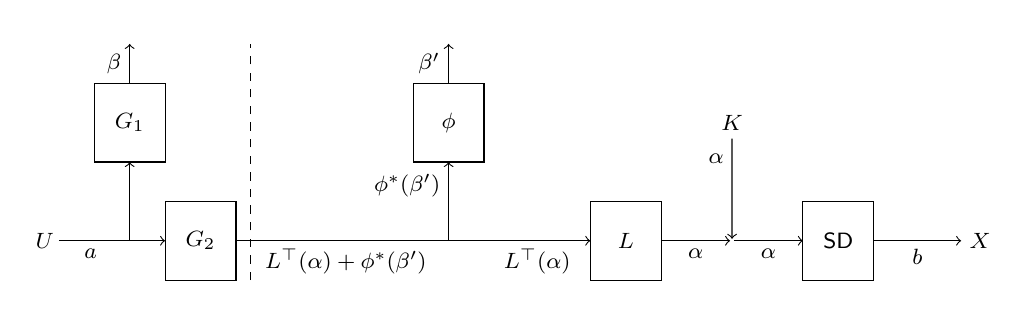
\begin{tikzpicture}[xscale=.9]
      \footnotesize
      % variables
      %\draw ( 2, 0) node(Xt){$X_{t}$} ;
      \draw (-1.7, 0) node(U){$U$} ;
      \draw (11.5, 0) node(Xtplus){$X$} ;
      \draw (8, 1.5) node(Kt){$K$} ;
      % \draw (4.5, 1.5) node(St){$S_t$};
      % operations
    \draw (-1, 1) rectangle +(1, 1) node[pos=0.5]{$G_{1}$} ;
  \draw ( 0, -0.5) rectangle +(1, 1) node[pos=0.5]{$G_{2}$};
      \draw (3.5, 1) rectangle +(1, 1) node[pos=0.5]{$\filter$} ;
      \draw ( 6, -0.5) rectangle (7, 0.5) node[pos=0.5]{$L$} ;
      \draw (8, 0) node(add)[inner sep=0pt]{$\boxplus$} ;
      \draw (9, -0.5) rectangle (10, 0.5) node[pos=0.5]{$\subW$} ;
      % arrows
      \draw[->] (-.5, 0) -- (-.5, 1) ;
      \draw[->] (-1.5, 0) --  node[below,pos=.3] { $\blue{a}$} (0, 0) ;
      \draw[->] (1, 0) --  node[below, pos=.31] { $\red{L^{\top}(\alpha) + \filter^{*}(\beta')}$} node[below, pos=.85] { $\red{L^{\top}(\alpha)}$} (6, 0) ;
      \draw[->] (4, 0) -- node[left,pos=.7] {$\red{\filter^{*}(\beta')}$} (4, 1) ;
      \draw[->] (7, 0) --  node[below] {$\red{\alpha}$} (add) ;
      \draw[->] (Kt) -- node[left,pos=.2] {$\blue{\alpha}$}(add) ;
      \draw[->] (add) -- node[below] {$\red{\alpha}$} (9, 0) ;
      \draw[->] (10, 0) --  node[below] {$\blue{b}$} (Xtplus) ;
      \draw[->] (4, 2) -- node[left,pos=.5] {\blue{$\beta'$}} (4, 2.5) node[above] {};
    \draw[->] (-.5, 2) -- node[left,pos=.5] {\blue{$\beta$}} (-.5, 2.5) node[above] {};
    \draw[dashed] (1.2,-.5) -- +(0, 3);
    % masks
    \end{tikzpicture}

  \caption{Masks propagation through a composition with \coolName{}'s round function. Input and output masks are written in blue while inner masks whose value are deduced are written in red.\label{fig:masks}}
\end{figure}
\begin{proof}
  For \(n\)~rounds, the Fourier coefficient $\widehat{F_{\alpha, \beta}}(0,\lambda)$ corresponds to a Fourier coefficient of the following function
    \[\begin{array}{rccl}
H^{(n)}: & \F_p^{16} \times \F_{p}^{16(n-1)} & \rightarrow & \F_{p}^{4(n-1)} \times \F_p^{16}\\
& (X_{0}, K_{1}, \ldots, K_{n-1}) & \mapsto & (S_0, \ldots, S_{n-2},X_{n-1})\;.
     \end{array}\]
 In other words, the output of \(H^{(n)}\) corresponds (up to a reordering of the 16 last digits) to the concatenation of the output of the augmented function \(F^{(n)}\) and of the remaining 12~internal digits that are not output by~$\filter$. % the last state of the FSM which are not outputted by~\(\filter\).
 Then, \(H^{(n+1)}\) can be seen as the composition of \(H^{(n)}\) with the round function
 \[\begin{array}{rcl}
 \F_p^{16} \times \F_p^{16} & \rightarrow & \F_p^4 \times \F_p^{16}\\
 (X_{n-1},K_n) & \mapsto & \left(\filter(X_{n-1}), \subW(L(X_{n-1})+K_n)\right)\end{array}\]
 Let \(G\) be any function of the form
 \[\begin{array}{rcl}
 G:\F_p^{\ell} & \rightarrow & \F_p^k \times \F_p^{16}\\
 U & \mapsto & (G_1(U),G_2(U))\end{array}\;.\]
 Then, the Fourier transform of the composition
 \[F:(U,K) \mapsto (G_1(U), \filter(G_2(U)), \subW(L(G_2(U))+K))\]
 can be easily derived from the Fourier transform of~\(G\), as shown on Figure~\ref{fig:masks}.
 Indeed, the detailed computation of the Fourier coefficient
 \[\mathcal{I} := {\widehat F}(a, \alpha;\beta, \beta', b)\]
 for the input mask \((a, \alpha)\) and output mask \((\beta, \beta', b)\) is as follows.
 \begin{eqnarray*}
   \mathcal{I} & = & \sum_{U \in \F_p^\ell,K \in \F_p^{16}} \omega^{\beta \cdot G_1(U) + \beta' \cdot \filter(G_2(U)) + b \cdot \subW(L(G_2(U))+K) - \alpha \cdot K - a \cdot U} \\
   & = & \sum_{U \in \F_p^\ell} \omega^{\beta \cdot G_1(U) + \beta' \cdot \filter(G_2(U))- a \cdot U} \left(\sum_{Z \in \F_p^{16}} \omega^{b \cdot \subW(Z) -\alpha \cdot Z+ \alpha \cdot L(G_2(U))}\right)
 \end{eqnarray*}
 where we set \(Z = L(G_2(U))+K\).
 We then deduce
 \begin{eqnarray*}
   \mathcal{I} & = & \sum_{U \in \F_p^\ell} \omega^{\beta \cdot G_1(U) + \beta' \cdot \filter(G_2(U))- a \cdot U + \alpha \cdot L(G_2(U))} {\widehat \subW}(\alpha, b)\\
   & = & {\widehat \subW}(\alpha, b)\sum_{U \in \F_p^\ell} \omega^{\beta \cdot G_1(U) + \filter^*(\beta') \cdot G_2(U)- a \cdot U + L^T(\alpha) \cdot G_2(U)} \\
   & = & {\widehat \subW}(\alpha, b) {\widehat G}(a ; \beta, L^T(\alpha) + \filter^*(\beta'))
   \end{eqnarray*}
 where \(\filter^*: \F_p^4 \rightarrow \F_p^{16}\) is the function outputting an internal state whose digits are all zero, expect the digits affected by \(\filter\), which are equal to the inputs.
       Finally, we observe that \(H^{(1)}\) is the identity function implying that \({\widehat H^{(1)}}(a,b) = p^{16}\) if \(a=b\) and \(0\) otherwise.
       It follows that the Fourier coefficients of \(H^{(n)}\) are either zero, or given by % \jb{Il manque pas un $\ind{a}(b'_{0})$ du coup comme premier terme ?}
       \[{\widehat H^{(n)}}(a, \alpha_1, \ldots \alpha_{n-1}; \beta_0, \ldots, \beta_{n-2}, b) = p^{16} \prod_{i=1}^{n-1} {\widehat \subW}(\alpha_{i}, b'_i) \;,\]
       for some \(b'_1, \ldots, b'_{n-1}\).
       Therefore,
       \[p^{-16n} {\widehat H^{(n)}}(a, \alpha_1, \ldots, \alpha_{n-1}; \beta_0, \ldots, \beta_{n-2}, b) = \prod_{i=1}^{n-1} \frac{{\widehat \subW}(\alpha_{i}, b'_i)}{p^{16}} \;.\]
 %Note that $\widehat{F_{\alpha, \beta}}(0,\lambda)$ corresponds to a particular case of $\widehat H^{(n)}$.
   The result then directly follows by observing that \({\widehat \subW}(\alpha_{i}, b'_i)\) is the product of the Fourier coefficients of the 16~\gls{S-box}es composing \(\subW\).
\hfil\qed
  \end{proof}

%% Let $(a, \alpha_1, ..., \alpha_{n}; \beta_0, ..., \beta_{n-1})$ be a vector of masks where the semi-colon separates input ones from output ones. Let us begin by proving that there exists \(b' \in \F_p^{16}\) such that
%%      % \noindent
%%      % \scalebox{0.86}{
%%      {\footnotesize
%%      \begin{equation*}
%%          {\widehat H^{(n+1)}}(a, \alpha_1, ..., \alpha_{n}; \beta_0, ..., \beta_{n-1}, b) ~=~
%%          {\widehat H^{(n)}}(a, \alpha_1, ..., \alpha_{n-1}; \beta_0, ..., \beta_{n-2}, b') \times {\widehat \subW}(\alpha_{n}, b) .
%%        \end{equation*}
%%      }

   
%%      Let \(\omega\) be a \(p\)-th root of unity in~\(\mathbb{C}\) and \(\chi(x) = \omega^x\) for \(x \in \F_p\). Then,
     
%%        \begin{eqnarray*}
%%          \mathcal{I} & = &   {\widehat H^{(n)}}(a,\alpha_1, \ldots, \alpha_{n-1}; \beta_0, \ldots, \beta_{n-2},b') \times {\widehat \subW}(\alpha_{n}, b) \\
%%                      & = & \sum_{X_0, K_1, \ldots, K_{n-1}} \chi\left(\sum_{i=0}^{n-2}\beta_i \cdot S_i + b'\cdot X_{n-1}- \sum_{i=1}^{n-1} \alpha_i \cdot K_i- a \cdot X_0\right) \sum_{Z} \chi\left(b \cdot \subW(Z) - \alpha_n \cdot Z\right) \\
%%                      & = & \sum_{X_0 ,K_1, \ldots, K_{n-1},K_n }   \chi\left(\sum_{i=0}^{n-2}\beta_i \cdot S_i + b' \cdot X_{n-1} - \sum_{i=1}^{n-1} \alpha_i \cdot K_i - a \cdot X_0\right)\\
%%        & & \hspace*{2cm} \times \chi\left(b \cdot \subW(K_n+L(X_{n-1})) - \alpha_n \cdot K_n - \alpha_n \cdot L(X_{n-1})\right)\;,
%%        \end{eqnarray*}
%%        where the variables summed over go through $\F_p^{16}$, and the last equality is obtained by setting \(Z = K_n + L(X_{n-1})\). Let \(\filter^*: \F_p^4 \rightarrow \F_p^{16}\) be the function outputting an internal state whose digits are all zero, expect the digits affected by \(\filter\), which are equal to the inputs. By exchanging the positions of $ b' \cdot X_{n-1}$ and $b \cdot X_{n} = b \cdot \subW(K_n+L(X_{n-1}))$, adding $\alpha_n \cdot K_n$ to the sum of $ \alpha_i \cdot K_i$, and adding $\beta_{n-1}\cdot S_{n-1} = \filter^*(\beta_{n-1}) \cdot X_{n-1}$ to the sum of $\beta_{i}\cdot S_{i}$, we deduce that \ac{Je trouve ca mega complique. Pourquoi pas simplement: We can rewrite \(\mathcal{I}\) as follows.}
%%       \begin{eqnarray*}
%%        \mathcal{I} 
%%        & = & \sum_{X_0, K_1, \ldots, K_{n} \in \F_p^{16}}  \chi\left(\sum_{i=0}^{n-1}\beta_i \cdot S_i + b \cdot X_n - \sum_{i=1}^{n} \alpha_i \cdot K_i - a \cdot X_0\right) \\
%%             & & \quad \times \chi\left(b' \cdot X_{n-1} -\filter^*(\beta_{n-1})\cdot X_{n-1}  - \alpha_n \cdot L(X_{n-1})\right).
%%            \end{eqnarray*}
%%            \begin{eqnarray*}
%%          & = & \sum_{X_0, K_1, \ldots, K_{n} \in \F_p^{16}}  \chi\left(\sum_{i=0}^{n-1}\beta_i \cdot S_i  + b \cdot X_n - \sum_{i=1}^{n} \alpha_i \cdot K_i - a \cdot X_0\right)\\
%%        & & \quad\times \chi\left((b'-\filter^*(\beta_{n-1}) - L^T(\alpha_n)) \cdot X_{n-1}\right) \\
%%      & = &    {\widehat H^{(n+1)}}(a,\alpha_1, \ldots, \alpha_n; \beta_0, \ldots, \beta_{n-1},b) \;,
%%          \end{eqnarray*}
%%        when \(b'=\filter^*(\beta_{n-1}) + L^T(\alpha_n)\) and \(L^T\) is the transpose of~\(L\). 


   


\subsection{Data Complexity of Fast Correlation Attacks}
\label{sec:fast-correlation-data}

It is well-known that the capacity of a linear approximation determines the minimal length of the sequence obtained by a given linear combination of the digits of \((S_t)_{t \in \mathbb{N}}\) that is required for recovering the initial state of the key-LFSR from the linear approximation
\[\sum_{i=1}^{n-1} \alpha_i \cdot K_{t+i} + \sum_{i=0}^{n-1} \beta_i \cdot S_{t+i}, \forall t \geq 0\;.\]

However, the same result holds even when the approximation is not linear as stated in the following theorem.
\begin{theorem}\label{th:Nmin}
  Let  \(F\) be a function from \(\F_p^\kappa \times \F_p^m\) to \(\F_p^n\). Let \(g:\F_p^\kappa \rightarrow \F_p\) and \(h: \F_p^n \rightarrow \F_p\) such that the probability distribution of
  \[(U,V) \mapsto h(F(U,V)) - g(U)\]
  is close to the uniform distribution, \ie, for all \(z \in \F_p\),
  \[\pr_{(U,V) \drawfrom \F_p^\kappa \times \F_p^m}[h(F(U,V)) - g(U)=z] = \frac{1}{p} + \varepsilon_z \mbox{ with } \varepsilon_z\ll 1\;.\]
  Let \((U_t)_{t \in \mathbb{N}}\) be a sequence of elements in~\(\F_p^\kappa\) defined by \(U_{t+1} = \Phi(U_t)\), where  $\Phi$ is a function from $\F_p^\kappa$ to itself. Let \((V_t)_{t \in \mathbb{N}}\) be a sequence of elements in~\(\F_p^m\).
  Then, the minimal length \(N\) of the sequence \( (B_{t})_{t \in \mathbb{N}} \vcentcolon= \left( h(F(U_t,V_t) \right)_{t \in \mathbb{N}}\) 
    required for recovering \(U_0\) is
  \[N = \frac{\kappa \ln p}{\Delta}\]
  with \[\Delta = p \sum_{y \in \F_p} \varepsilon_y^2 = \sum_{a \in \F_p^*} \left|p^{-\kappa} \sum_{U \in \F_p^\kappa,V\in \F_p^m}\omega^{a(h(F(U,V)) - g(U))}\right|^2\;.\]
\end{theorem}
\begin{proof}
  Let
  \[\mathcal{C} = \{(g(\Phi^t(U_0)))_{0 \leq t < N}, U_0 \in \F_p^\kappa\}\;.\]
  This set is a (non-linear) code over \(\F_p\) of length~\(N\) and size \(p^\kappa\).
  As originally observed by Meier and Staffelbach~\cite{EC:MeiSta88}, recovering \(U_0\) from \((B_0, \ldots, B_{N-1})\) boils down to decoding this code. Indeed, \((B_0, \ldots, B_{N-1})\) can be seen as the result of the transmission of the \(N\)-digit word \((g(U_0), \ldots, g(\Phi^{N-1}(U_0)))\)  through a noisy transmission channel. This transmission channel is memoryless, since each digit is affected in the same way:
  \[B_t = g(\Phi^{t}(X_0)) + \eta_t\]
  where the probability distribution of all \(\eta_t\) is given by
  \[\pi_z := \pr[\eta_t = z] = \pr_{(U,V) \drawfrom \F_p^\kappa \times \F_p^m}[h(F(U,V)) - g(U)=z]= \frac{1}{p} + \varepsilon_z\;.\]
  This transmission channel is called symmetric in the sense that its transition matrix, formed by the probabilities that an input value~\(i\) is transformed to~\(j\), is a circulant matrix whose rows correspond to the probability distribution \((\pi_0, \ldots, \pi_{p-1})\).
  Therefore, Shannon's channel-coding theorem~\cite[Section~7.7]{add:CovTho06} implies that this code can be decoded with a non-negligeable success probability if and only if its rate, \ie, the ratio between the logarithm of its size and its length, is smaller than the channel capacity:
  \[\frac{\kappa}{N} \leq C_{\mathrm{channel}}\;.\]
  The capacity of any \(p\)-ary symmetric channel is given by~\cite[Th.~7.2.1]{add:CovTho06}
  \[C_{\mathrm{channel}} = 1 - H_p(\pi_0, \pi_1, \ldots, \pi_{p-1})\]
  where \(H_p\) denotes the \(p\)-ary entropy, i.e.,
  \[H_p(\pi_0, \pi_1, \ldots, \pi_{p-1}) := - \sum_{z \in \F_p} \pi_z \log_p(\pi_z)\;.\]
  We use that, for \(\varepsilon \ll 1\),
  \[\ln\left(\varepsilon + \frac{1}{p}\right) = \ln(1 + p \varepsilon) - \ln p = p \varepsilon - \ln p + o(\varepsilon)\;.\]
  It follows that
  \begin{eqnarray*}
    \sum_{z \in \F_p} \left(\varepsilon_z + \frac{1}{p}\right) \ln\left(\varepsilon_z + \frac{1}{p}\right) & \simeq & p \sum_{z \in \F_p} \varepsilon_z^2 - \ln p \sum_{z \in \F_p} \left(\varepsilon_z + \frac{1}{p}\right)\;.
  \end{eqnarray*}
  We then deduce that
  \[C_{\mathrm{channel}} = 1 + \frac{1}{\ln p} \left(p \sum_{z \in \F_p} \varepsilon_z^2  -\ln p\right) = \frac{1}{\ln p} \left(p \sum_{z \in \F_p} \varepsilon_z^2\right)\;.\]
  It is well-known (see Prop.~\ref{prop:capa}) that the same quantity can also be derived from the Fourier transform of the function
  \[f: (U,V) \mapsto h(F(U,V)) - g(U)\;.\]
  Indeed, if \(\pi'\) denotes the function from \(\F_p\) to \(\mathbb{R}\) defined by \(\pi'(x) = \pi_x - \frac{1}{p} = \varepsilon_x\), we have
    \[\Delta = p \sum_{y \in \F_p} \left|\pi'(y)\right|^2 = \sum_{a \in \F_p} \left|{\widehat \pi'}(a)\right|^2\]
    where the last equality corresponds to Plancherel's formula.
    Moreover, the Fourier transform of~\(\pi'\) an be computed as follows: if \(a \neq 0\),
    \begin{eqnarray*}
      {\widehat \pi'}(a) & = & \sum_{x \in \F_p} \pi'(x) \omega^{-ax} = \sum_{x \in \F_p} \pi_x \omega^{-ax} - p^{-1} \sum_{x \in \F_p} \omega^{-ax}\\
      & = & p^{-(\kappa+m)} \sum_{x \in \F_p} \#f^{-1}(x) \omega^{-ax} = p^{-(\kappa+m)} \sum_{U,V \in \F_p^\kappa \times \F_p^m}  \omega^{-a f(U,V)}
      \\ & = & p^{-(\kappa+m)} {\widehat f}(0, -a)\;,
      \end{eqnarray*}
    and \({\widehat \pi'}(0) = 0\).
        It follows that
        \[\Delta = \sum_{a \in \F_p^*} \left|p^{-(\kappa+m)} {\widehat f}(0, a)\right|^2\;.\]
        \hfil\qed
\end{proof}



% Leo: ce qui suit est pour qu'emacs compile bien l'article, pas touche !
%%% Local Variables:
%%% mode: latex
%%% ispell-local-dictionary: "english"
%%% TeX-master: "main"
%%% End:

%\section{More Resources About TFHE}
\label{sec:appendix_fhe}


\subsection{Complexity assumptions}
\label{sec:complexity_assumptions}

Here, we define the assumptions on which the security of TFHE relies. 

\begin{definition}
	(LWE problem over the discretized torus). Let $q, n \in \mathbb N$ and let $\vec s = (s_1, \dots, s_n) \drawfrom \mathbb B^n$. Let $\chi$ be an error distribution over $\mathbb Z_q$. The \emph{decisional Learning With Errors over discretized torus problem} is to distinguish between samples drawn from the distributions: 
	\[
	\mathcal{D}_0 = \{(\vec a, r)\mid\vec a \drawfrom \mathbb T_q^n, r \drawfrom \mathbb T_q\}
	\] and: \[
	\mathcal{D}_1 = \{(\vec a, b)\mid\vec a = (a_1, \dots, a_n) \drawfrom \mathbb T_q^n, e \drawfrom \chi, b = \sum_{j=1}^n a_j \cdot s_j + e\}.
	\]
	The \emph{search} version of the problem is to recover $\vec s$ from samples of $\mathcal{D}_1$.
	\label{def:LWE}
\end{definition}
Both the search and decisional problems are reducible to each other \cite{Regev}, and their average case is as hard as the worst-case lattice problems.


TFHE also relies on the generalized version of LWE over rings, introduced in \cite{ITCS:BraGenVai12}, known as GLWE.

\begin{definition}
	(GLWE problem over the discretized torus). Let $N, q, k \in \mathbb N$ with $N$ a power of two and let $\vec s = (s_1, \dots, s_k) \drawfrom \mathbb B_N[X]^k$. Let $\chi$ be an error distribution over $\mathbb Z_{N, q}[X]$. The \emph{General decisional Learning With Errors over discretized torus problem} is to distinguish between samples drawn from the following distributions 
	\[
		\mathcal{D}_0 = \{(\vec a, r) \mid \vec a \drawfrom \mathbb T_{N, q}[X]^k, r \drawfrom \mathbb T_{N, q}[X]\}
		\]
		
		and: \[\mathcal{D}_1 = \{(\vec a, b) \mid \vec a = (a_1, \dots, a_k) \drawfrom \mathbb T_{N, q}[X]^k, e \drawfrom \chi, b = \sum_{j=1}^k a_j \cdot s_j + e\}.
	\]
	\label{def:GLWE}
	The \emph{search} version is analogous to the LWE one.
\end{definition}
%
The complexity analysis is analogous to the LWE version.
In practice, the error distribution $\chi$ is a centered Gaussian distribution parametrized by its standard deviation $\sigma$.





\subsection{Analysis of the variances inside a PBS}
\label{sec:pbs_variance_analysis}

We recall that the PBS is composed of four successive operations: \textsf{Keyswitch}, \textsf{ModulusSwitch}, \textsf{BlindRotate} and \textsf{SampleExtract}.


The critical variance is the variance in input of the \textsf{BlindRotate} (\textsf{BR}). If the noise at this point of the algorithm is too high, the PBS will output the encryption of a wrong value with high probability. This critical variance satisfies:
$$\sigma^2_{\text{in-}\textsf{BR}} = \sigma^2_{\text{in-}\textsf{PBS}} + \sigma^2_{\textsf{KS}} + \sigma^2_{\textsf{MS}}$$
where $\sigma^2_{\text{in-}\textsf{PBS}}$ is the variance in input of the PBS, which according to Section~\ref{sec:rationale-controllin-noise} satisfies:
$$\sigma^2_{\text{in-}\textsf{PBS}} = \sigma_\pseudoKS^2+\sigma^2_\mixC = 
|\mathcal{K}| \cdot \left(\frac{p-1}2\right)^2 \cdot \sigma_{\text{long}}^2 + L_\mixC^2 \cdot \sigma^2_{\textsf{PBS}}~,$$
and where $\sigma^2_{\textsf{KS}}$ and $\sigma^2_{\textsf{MS}}$ are additive terms introduced by the $\textsf{KeySwitch}$ and the $\textsf{ModSwitch}$ respectively and which depend on the internal parameters of the PBS. The former is defined by:
%
\begin{equation*}
	\begin{aligned}
		\sigma_{\sf{KS}}^2 & = n_{\text{long}} \cdot \left( \frac{q^2}{12B_{\text{KS}}^{2\ell_{\text{KS}}}} - \frac{1}{12} \right) \cdot \left( \text{Var}(s_i) + \mathbb{E}^2(s_i) \right) \\
		& + \frac{n_{\text{long}}}{4} \cdot \text{Var}(s_i) + n_{\text{long}} \cdot \ell_{\sf{KS}} \cdot \sigma_{\sf{KSK}}^2 \cdot \frac{B_{\text{KS}} + 2}{12}
	\end{aligned}
\end{equation*}

where $s_i$ refers to the secret key's bits used for encryption, and $\sigma_{\sf{KSK}}$ is the noise introduced in the key-switching keys (so $\sigma_{\text{short}}$ in our case).

For $\sigma_{\textsf{MS}}$, we have:
\begin{equation*}
	\sigma^2_{\sf{MS}} = \frac {q^2} {4 N^2} \cdot \left ( \frac{1}{12} - \frac{4N^2}{12 q^2} + \frac{n_{\text{short}}}{24} + \frac{n_{\text{short}} \cdot 4 N^2}{48 q^2} \right )
\end{equation*}

The full noise analysis leading to these formulas can be found in \cite{phd_tap}.


\ifeprint{
	\section{Further Compressing the TFHE Ciphertexts}
	\label{sec:truncature}

}
\else{
	\section{More about the Homomorphic Implementation of Transistor}
	
	
	\subsection{Further Compressing the TFHE Ciphertexts}
	\label{sec:truncature}
}
\fi

We introduce hereafter a tweak to compress a TFHE encryption further than the folklore compression. By definition of the TFHE encryption process, the least significant bits of the body $b_i = \sum_{j=1}^n a_{i,j} \cdot s_j + \tilde{m}_i + e_i$ are randomized by the error $e_i$ and can hence be discarded without loss of information. We can thus tweak the above compressed encryption process by returning $(\mathsf{seed}, \mathrm{Tr}_\ell(b_1), \ldots, \mathrm{Tr}_\ell(b_t))$ where $\mathrm{Tr}_\ell(\cdot)$ denotes the truncation of the $\ell$ least significant bits. To decompress such ciphertexts, besides pseudorandomly generating the masks from the seed, one just needs to pad the truncated bodies with $\ell$ bits to $0$. By the randomness of the mask, the effect of this truncation plus $0$-padding is to add a uniform random error of $\ell$ bits to the body, namely an error of standard deviation: 
$$\sigma_0^2  = \frac{(2^\ell - 1)^2}{12} \approx \frac{2^{2\ell}}{12} \approx 0.08 \cdot 2^{2\ell} ~.$$

\noindent This optimization comes in two flavors:
\begin{enumerate}
	\item \emph{The ``free'' variant.} The number of truncated bits $\ell$ is selected to have a small impact on the noise distribution. For instance in \coolName, the noise of the fresh ciphertexts is summed with the noise coming from the FSM. Thus, we can compute $\ell$ to keep $\sigma^2_{\mathcal W} < \sigma^2_{\text{PBS}}$. Our experiments shows $\sigma^2_{\text{PBS}} = 2^{52}$, so running the numbers we find that we can truncate up to $\ell=19$ bits, allowing to reduce the volume of the TFHE ciphertexts to send by a factor $1 - \frac{19}{64} \approx 0.7$.
	
	\smallskip
	
	\item \emph{The communication-computation trade-off.} In this variant, one selects a high value of $\ell$. The truncated body should at least contain $\log_2(p)$ bits to keep the plaintext information, plus a margin of a few bits in order to remain bootstrappable. Denoting this margin $\delta$, the truncated body should be of at least $\log_2(p) + \delta$ bits and $\ell$ can be up to $\log_2(q) - (\log_2(p)+\delta)$. Taking the maximum level of truncation, inducing the maximum level of bootstrappable noise, implies some adaptation of the underlying homomorphic computation. Specifically, it should start with applying a noise-reduction bootstrapping to the decompressed ciphertexts before performing the original evaluation. We hence obtain a trade-off with reduced bandwidth against additional bootstrappings.
\end{enumerate}

In the context of transciphering with \coolName, the trade-off provided by the second option gives rise to an initialization procedure which consists in decompressing and bootstrapping the wrapped key. 


\ifeprint{

}
\else{
	
	\subsection{Overview of the Shapes of the Ciphertexts used in \coolName}
	\label{sec:schema_structure_fhe}
	
	In the different steps of the homomorphic evaluation of \coolName, ciphertexts of several types and forms are used. They are illustrated in Figure \ref{fig:structure_fhe}.
	
	\begin{figure}[t!]
  \centering
    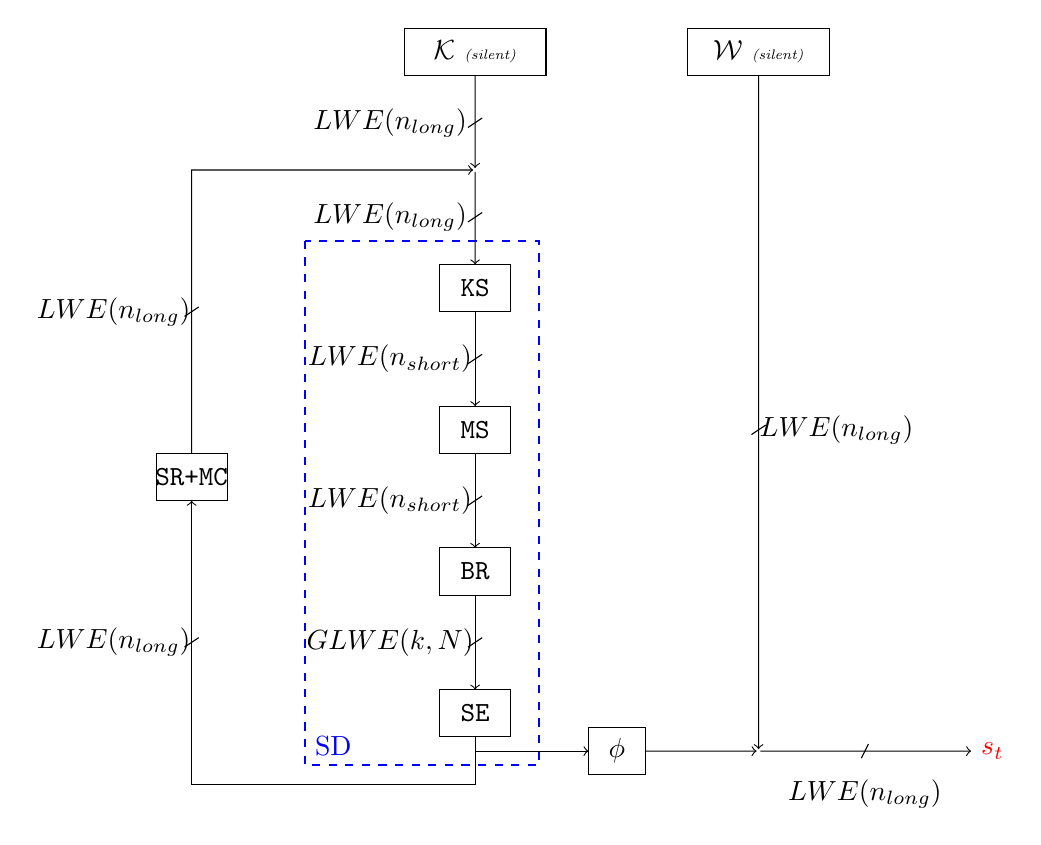
\begin{tikzpicture}[xscale=0.9,yscale=0.6]
 
    %LSFRs
    \draw[] (0, 0) rectangle (2, 1) node[pos=0.5]{$\pseudoKS$ {\tiny \emph{(silent)}}} ;
    \draw[] (4, 0) rectangle (6, 1) node[pos=0.5]{$\whitening$ {\tiny \emph{(silent)}}} ;
    \draw (1, -2) node[inner sep=0pt](addm){$\boxplus$} ;
    \draw[->] (1, 0) -- (addm);

    % FSM
    \draw[] (0.5, -4) rectangle (1.5, -5) node[pos=0.5,color=black](ks){$\texttt{KS}$} ;
    \draw[] (0.5, -7) rectangle (1.5, -8) node[pos=0.5,color=black](ms){$\texttt{MS}$} ;
    \draw[] (0.5, -10) rectangle (1.5, -11) node[pos=0.5,color=black](br){$\texttt{BR}$} ;
    \draw[] (0.5, -13) rectangle (1.5, -14) node[pos=0.5,color=black](se){$\texttt{SE}$} ;
    \draw[] (-3.5, -8) rectangle (-2.5, -9) node[pos=0.5,color=black](srmc){$\texttt{SR+MC}$} ;

    % Draw dashed blue box for SB
    \draw[dashed, blue, thick] (-1.4, -3.5) rectangle (1.9, -14.6);
    \node[blue] at (-1, -14.2) {SD}; % Label for the box

    % FSM connections
    \draw[->] (addm) -- (1, -4);
    \draw[->] (1, -5) -- (1, -7);
    \draw[->] (1, -8) -- (1, -10);
    \draw[->] (1, -11) -- (1, -13);
    \draw[->] (1,-14) -- (1, -15) -- (-3, -15) -- (-3, -9);
    \draw[->] (-3, -8) -- (-3, -2) -- (addm);

    % Extraction
    \draw (5, -14.3) node[inner sep=0pt](addr){$\boxplus$} ;
    \draw[] (2.6, -13.8) rectangle (3.4, -14.8) node[pos=0.5,color=black]{$\phi$} ;

    \draw[->] (1, -14.3) -- (2.6, -14.3);
    \draw[->] (3.4, -14.3) -- (addr);
    \draw[->] (5, 0) -- (addr);
    \draw[->] (addr) -- (8, -14.3);
    \draw[color=red] (8.3, -14.3) node(s){$s_t$} ;



    % Wire type
    \draw (0.9, -1.1) -- (1.1, -0.9) ;
    \draw (-0.2, -1) node{$LWE(n_{\text{long}})$} ;
    \draw (0.9, -3.1) -- (1.1, -2.9) ;
    \draw (-0.2, -3) node{$LWE(n_{\text{long}})$} ;
    \draw (0.9, -6.1) -- (1.1, -5.9) ;
    \draw (-0.2, -6) node{$LWE(n_{\text{short}})$} ;
    \draw (0.9, -9.1) -- (1.1, -8.9) ;
    \draw (-0.2, -9) node{$LWE(n_{\text{short}})$} ;
    \draw (0.9, -12.1) -- (1.1, -11.9) ;
    \draw (-0.2, -12) node{$GLWE(k, N)$} ;
    \draw (-3.1, -12.1) -- (-2.9, -11.9) ;
    \draw (-4.1, -12) node{$LWE(n_{\text{long}})$} ;
    \draw (-3.1, -5.1) -- (-2.9, -4.9) ;
    \draw (-4.1, -5) node{$LWE(n_{\text{long}})$} ;
    \draw (4.9, -7.6) -- (5.1, -7.4) ;
    \draw (6.1, -7.5) node{$LWE(n_{\text{long}})$} ;
    \draw (6.45, -14.45) -- (6.55, -14.15) ;
    \draw (6.5, -15.2) node{$LWE(n_{\text{long}})$} ;

    \end{tikzpicture}
  \vspace{1em}
  \hfill~
  \caption{\label{fig:structure_fhe} Types and shapes of ciphertexts in homomorphic \coolName. The $\subWords$ is broken down into its elementary components}
\end{figure}


% Leo: ce qui suit est pour qu'emacs compile bien l'article, pas touche !
%%% Local Variables:
%%% mode: latex
%%% ispell-local-dictionary: "english"
%%% TeX-master: "../main"
%%% End:




	
}
\fi





\ifeprint{


}
\else{
	\subsection{Concrete Parameters}
	\label{sec:concrete_parameters}
	
	Table \ref{tab:parameters} shows the parameters used for our experiments, all ensuring 128 bits of security. The obtained security levels $\lambda_{\text{short}}$ et $\lambda_{\text{long}}$ have been estimated using the \texttt{lattice estimator}~\cite{lattice-estimator}.
	
	\begin{table}
		\centering
		\caption{TFHE Parameters used in our experimentations}.
			\label{tab:parameters}
		\renewcommand{\arraystretch}{1.3}  % Adjust row spacing
		\scalebox{1}{
			\begin{tabular}{|c||*{12}{>{\centering\arraybackslash}p{0.8cm}|}}
				\hline
				$p_{\text{err}}$ & $q$ & $n_{\text{short}}$ & $k$ & $N$ & $\sigma_{\text{short}}$ & $\sigma_{\text{long}}$ & $B_{BR}$ & $\ell_{\text{BR}}$ & $B_{KS}$ & $\ell_{\text{KS}}$ & $\lambda_{\text{short}}$ & $\lambda_{\text{long}}$\\
				\hline
				$2^{-40}$ & $2^{64}$ & 788 & 2 & 1024 & $2^{47}$ & $2^{14}$ & $2^{23}$ & 1 & $2^4$ & 3 & 131.8 & 128.9\\
				\hline
				$2^{-128}$ & $2^{64}$ & 774 & 1 & 2048 & $2^{47}$ & $2^{14}$ & $2^{23}$ & 1 & $2^3$ & 5 & 131.8 & 128.9\\
				\hline
		\end{tabular}}
		
	\end{table}
}
\fi

\ifeprint{
	
}
\else{
	\subsection{Detailed Homomorphic Implementations}
	\label{sec:detailed_implementation}
	
	In the following, we provide a more detailed way of how we implemented the homomorphic version of \coolName.
	
	\paragraph{Homomorphic evaluation of LSFRs.}
	The \coolName design involves two LSFRs operating on elements of $\field{17}$. The standard way to implement an LSFR is to evaluate the linear feedback function on the state at each clock cycle, thus producing a new element that enters the state, while the state is shifted to output an element. 
	%generate the new element at each clock cycle, and then to mutate the state by shifting the elements of the state and compute the linear combination of the state with the coefficients of retroaction to produce a new one.
	We suggest the \emph{silent LFSR} approach for the homomorphic evaluation of LFSRs. In this approach, the encrypted LFSR state is immutable to avoid any noise growth in the underlying ciphertexts (hence keeping the LFSR ``silent''). We use the fact that every output element of the LFSR can be expressed as a linear combination of the initial state. So, at each clock cycle, we compute \emph{in the clear} the coefficients of this linear combination and homomorphically evaluate it on the immutable encrypted state. This process is depicted in Algorithm~\ref{alg:lsfr}.
	
	\begin{algorithm}[t!]
    \caption{\texttt{LFSR.clock} - Produce a pseudo random element of the state. \label{alg:lsfr}}
    
    \KwIn{
        $\left\{
        \begin{aligned}
            &\ell: \text{ Size of the state of the LFSR.} \\
            &(u_1, \dots, u_\ell): \text{ Encrypted initial state of the LFSR.} \\
            &(\lambda_1^{(0)}, \dots, \lambda_\ell^{(0)}): \text{ Coefficients of retroaction in the definition of the LFSR.} \\
            &(\lambda_1^{(i)}, \dots, \lambda_\ell^{(i)}): \text{ Previous coefficients used in the linear combination.}
        \end{aligned}
        \right.$
    }

    \KwResult{
        $\left\{
        \begin{aligned}
            &o^{(i)}: \text{ Encryption of the $i$-th pseudorandom element of $\F_{17}$.} \\
            &(\lambda_1^{(i+1)}, \dots, \lambda_\ell^{(i+1)}): \text{ Updated coefficients of the linear combination.}
        \end{aligned}
        \right.$
    }

    % Add vertical space and horizontal line
    \vspace{0.5em} % adjust the space as needed
    \hrule
    \vspace{0.5em} % adjust the space as needed

    $o^{(i)} \gets 0$

    \Comment{Evaluation of the linear combination}
    \For{$k \in \{1, \dots, \ell\}$}{
        $o^{(i)} \gets \texttt{SumTFHE}(o^{(i)}, \texttt{ClearMultTFHE}(u_k, \lambda_k^{(i)}))$
    }
    \Comment{Update of the next coefficients}
    \For{$k \in \{2, \dots, \ell\}$}{
        $\lambda_k^{(i+1)} \gets \lambda_{k-1}^{(i)} + \lambda_\ell^{(i)} \cdot \lambda_k^{(0)}$
    }
    $\lambda_1^{(i+1)} \gets \lambda_\ell^{(i)} \cdot \lambda_1^{(0)}$
    
    \Return{$o^{(i)}$}
    
\end{algorithm}


	
	%Calling Algorithm \ref{alg:lsfr} (\texttt{LFSR.clock}) several times yields an encrypted stream of pseudorandom elements $(o^{(0)}, o^{(1)}, \dots)$.
	
	\paragraph{Homomorphic evaluation of} \coolName. The complete homomorphic evaluation of a round of one clock cycle of \coolName is depicted in Algorithm~\ref{alg:transistor}, using $\pseudoKS.\texttt{clock}$ and $\whitening.\texttt{clock}$ as subroutines (i.e., Algorithm~\ref{alg:lsfr} evaluated on the key schedule and whitening LFSRs). The most computation intensive part of the algorithm is by far the evaluation of the PBS in $\subWords$ which can be fully parallelized to reduce the latency.
	
	\begin{algorithm}[t!]
    \caption{\texttt{Transistor.clock} - Produce $r$ encypted elements of the key stream}
    \label{alg:transistor}
    
 
    \KwIn{
        $\left\{
        \begin{aligned}
        	&\mathcal K: \text{the LFSR used for the pseudo-keyschedule and its state (cf Algorithm \ref{alg:lsfr}).}\\
            &\mathcal W: \text{the LFSR used for the whitening.}\\	
            &X = \left ( \begin{array}{ccc}
            x_{1,1} & \dots & x_{1,\sqrt{m}}\\
            \dots & \dots & \dots\\
            x_{\sqrt{m},1} & \dots & x_{\sqrt{m},\sqrt{m}}\\
            \end{array} \right ): \text{ Encrypted state of the FSM} \\
        \end{aligned}
        \right.$
    }

    \KwResult{
        $\left\{
        \begin{aligned}
            &Y = (y_1, \dots, y_r): \text{ Encryption of $r$ elements of the  key stream } \\
        \end{aligned}
        \right.$
    }

    % Add vertical space and horizontal line
    \vspace{0.5em} % adjust the space as needed
    \hrule
    \vspace{0.5em} % adjust the space as needed

    \Comment{Compute the pseudo-key schedule and adds it to the FSM}
    \For{$i \in [1, \sqrt m]$}{
        \For{$j \in [1, \sqrt m]$}{
            $k_{i,j} \gets \pseudoKS.\texttt{clock}()$\\
            $x_{i,j} \gets \texttt{SumTFHE}(x_{ij}, k_{i,j})$\\
        }
    }
    \Comment{Compute $\subWords$ with a layer of PBS}
    \For{$i \in [1, \sqrt m]$}{
        \For{$j \in [1, \sqrt m]$}{        
            $x_{i,j} \gets \texttt{PBS\_TFHE}(x_{i,j}, S)$\\
        }
    }
    \Comment{Extract the output bits and whiten them}
    $(y_1, \dots, y_r) \gets \phi(X)$\\
    \For{$i \in [1, r]$}{
        $w_i \gets \whitening.\texttt{clock}()$\\
        $y_i \gets \texttt{SumTFHE}(y_i, w_i)$\\
    }
    \Comment{Compute $\shiftRows$, (same as in clear)}
    $X \gets \shiftR(X)$

    \Comment{Compute MixColumns}
    \For{$i \in [1, \sqrt m]$}{
        \For{$j \in [1, \sqrt m]$}{
            $z_{i, j} \gets 0$\\
            \For{$k \in [1, \sqrt m]$}{
                $z_{i, j} \gets \texttt{SumTFHE}(z_{i, j}, \texttt{ClearMultTFHE}(x_{k, j}, MC_{i, k}))$\\
            }
        }
    }

    \Return{$Y$}

\end{algorithm}


	}
\fi

\ifeprint{

}
\else{
	\subsection{Size of the server key}
	\label{sec:server_key_sizes}
	We  provide the sizes for the server keys in Table \ref{tab:server_key_size}, namely the \emph{key-switching key} (KSK) and the \emph{bootstrapping key} (BSK) while using the ciphertext compression technique described in Section~\ref{sec:key_wrapping}. Those keys are only generated and communicated to the server once (during some user enrolment step).
	
	
	
	\begin{table}
		\centering
		\caption{Size of the server keys for the two considered sets of parameters. 
			%This is agnostic to the volume of message sent. 
			\label{tab:server_key_size}}
		
		\renewcommand{\arraystretch}{1.2}  % Adjust row spacing
		\scalebox{0.9}{
			\begin{tabular}{|c||*{3}{>{\centering\arraybackslash}p{4cm}|}}
				\hline
				& Theoretical sizes & Sizes for $p_{\text{err}} = 2^{-40}$ & Sizes for $p_{\text{err}} = 2^{-128}$ \\
				\hline
				~KSK~ &  $n_{\text{long}}\cdot l_{\text{KS}} \cdot \log_2 q $ & 49 KB & 82 KB  \\
				\hline
				~BSK~ &  $n_{\text{short}} \cdot l_{\text{BS}} \cdot \log_2 q \cdot N \cdot (k+1)$ & 6.5 MB & 12.7 MB  \\
				\hline
		\end{tabular}}
		
	\end{table}
}
\fi



%% !TeX root = ./main.tex
\section{Additionnal Cryptanalysis}
\label{sec:appendix-cryptanalysis}



\subsection{Algebraic Analysis}
\label{sec:cryptanalysis-algebraic}
Algebraic cryptanalysis consists of formulating nonlinear equations that an attacker can derive from the information observed in terms of the secret key material. Several techniques, such as Gröbner basis methods or linearization, exist for solving such systems of equations, and we discuss them in this section. Based on this analysis, we claim that \coolName{} is resistant to algebraic attacks and their improvements.

%A first generic approach can be to rely on a Gröbner basis. A second generic approach can be to use linearization technique, that is considering any multivariate monomial involved in the system as new and independent variable also be to and a second approach to attacks based on deriving low-degree equations in the internal state from the observation of the keystream. We also discuss linearization techniques further below.


\paragraph{Gröbner Basis.} Such an attack consists of four main steps: formulating the equations that model the intended cryptanalysis, computing their Gröbner basis, applying a ``change of monomial ordering'' to transform the Gröbner basis into a more useful form, and finally solving the result using univariate techniques. The complexity of the first and last steps is usually negligible, meaning that we should evaluate the time complexity of at least one of the other two steps.

However, as recently shown in~\cite{C:BBLAOP24}, it is possible to write the equations in such a way as to entirely bypass the computation of the Gröbner basis. This is achieved by choosing a custom \emph{monomial ordering} that ensures the equations, as formulated, immediately form a Gröbner basis. This approach can be applied here by assigning increasing weights to the successive outputs of the key schedule, so that the leading monomials in each equation involve only a single key variable. This method is effective for at least the first four clock cycles, as the clock outputs are independent.

At this stage, we have 16 independent equations of degree 15 (the degree of $\thesbox$). Adding the equations corresponding to the next $20$ clocks, we get as many equations as unknowns, which, in particular, should lead to a 0-dimensional ideal. As conjectured in~\cite{EPRINT:Perrin24}, the ideal degree of this system can be lower-bounded by $15^{16} \approx 2^{62.5}$. This bound would be exact if the 80 remaining equations somehow failed to contribute to an increase in this quantity, or if the ideal degree was in some way decreased by one of these equations (despite the 0-dimension). Given that change of order algorithms are at least quadratic in the ideal degree, we can safely claim security against Gröbner-basis-based algebraic attacks.

%\paragraph{Classical Algebraic Attack.} \lp{todo. On dit qu'on s'en fout parce que faire 0 dans $\mainField$ ça dit pas grand chose?}\yr{Oui, on s'en fout}


\paragraph{Linearization.}Such attacks may, a priori, pose a threat, as they have led to the downfall of two \gls{FHE}-friendly stream ciphers, namely {\tt FLIP}~\cite{EC:MJSC16} and {\tt Elisabeth}~\cite{AC:CHMS22}, which were broken in~\cite{C:DuvLalRot16} and~\cite{AC:GBJR23}, respectively. The structure of these ciphers made such attacks an inherent risk: in both cases, a low-degree function is applied to a constant key register to generate keystream words.  As a result, in these ciphers, the nonlinear equations derived from the keystream sequence have a constant degree. Considering all monomials (or linear combinations of monomials) as new independent variables in this representation enables powerful attacks~\cite{C:DuvLalRot16,AC:GBJR23}. These attacks are the result of  two fundamental weaknesses: the constant degree of the system and low diffusion, as the registers are never updated, only a bit-permutation is applied at each clock cycle.

These issues are directly addressed in the design of \coolName{}. First, the round function of the FSM applies the S-box \( \thesbox \) to every digit. This S-box has a univariate representation in \( \mainField \) that is both dense and of degree 15. Furthermore, the content of the FSM accumulates high-degree equations within the key-LFSR. As a result, the multivariate polynomial representation of the keystream digits will not have a constant degree; instead, it will be very dense and of high degree.


\paragraph{Using Annihilators.} Another powerful technique is to directly use an annihilator of the filtering function, where this annihilator has a lower degree than the original function~\cite{EC:CouMei03,C:Courtois03}. This allows the attacker to collect and solve a system of equations with a smaller degree than the original one. That is, similar to Gröbner basis-like attacks, this approach operates on the ideal generated by the polynomials. In the case of \coolName{}, we can argue and defend the role of the whitening LFSR \( \whitening \). Indeed, this LFSR has a length of 32 digits, meaning that an annihilator at the output must consider the sum of 8 outputs by \( \phi \) and cancel them with a polynomial. Therefore, without additional information, such an annihilator would need to multiply approximately 32 digits, leading to an increase in the degree. This strategy must also account for the degree increase in successive outputs of \( \phi \), as discussed above.

\paragraph{Other Techniques.}
Last but not least, algebraic attacks can be improved in several ways using the Guess-and-Determine strategy or the so-called Hybrid approach in Gröbner basis computations. In our case, one could guess key-register cells, whitening-key cells, or cells in the FSM. Although this is a valid approach, the remaining equations (depending on the guessing strategy) would either have an increased degree or require guessing too many cells, making the attack impractical.



\subsection{Comparison With {\tt LEX}}
\label{sec:security-lex}

{\tt LEX}~\cite{SAC:Biryukov06} is a stream cipher designed by Biryukov in 2006 and selected to the third phase of the eSTREAM competition. {\tt LEX} employed a rather unusual design for a stream cipher, based on the {\tt \gls{AES}} block cipher and a technique called \emph{leak extraction}. The idea of the leak extraction is to produce the key stream by extracting parts of the underlying block cipher state.

The description of {\tt LEX} is very simple and elegant. It is based on a slightly tweaked version of the {\tt \gls{AES}} where the {\sf AddRoundKey} operation before the first round is omitted and where the {\tt MixColumns} of the last round is not. For simplicity, we will still refer to this tweaked version as {\tt \gls{AES}}. First, the publicly known $IV$ is encrypted by the {\tt \gls{AES}} under the secret key $K$ to produce an initial state  $S = {\tt \gls{AES}}_K(IV)$. Then, the state $S$ is repeatedly encrypted using the OFB mode and the same secret key $K$. At each round of encryption, four words of the internal state are extracted to compose the key stream produced by {\tt LEX}. The positions of the extracted words depend on the round number and are depicted in Figure~\ref{fig:lex}.

\begin{figure}
  \centering
  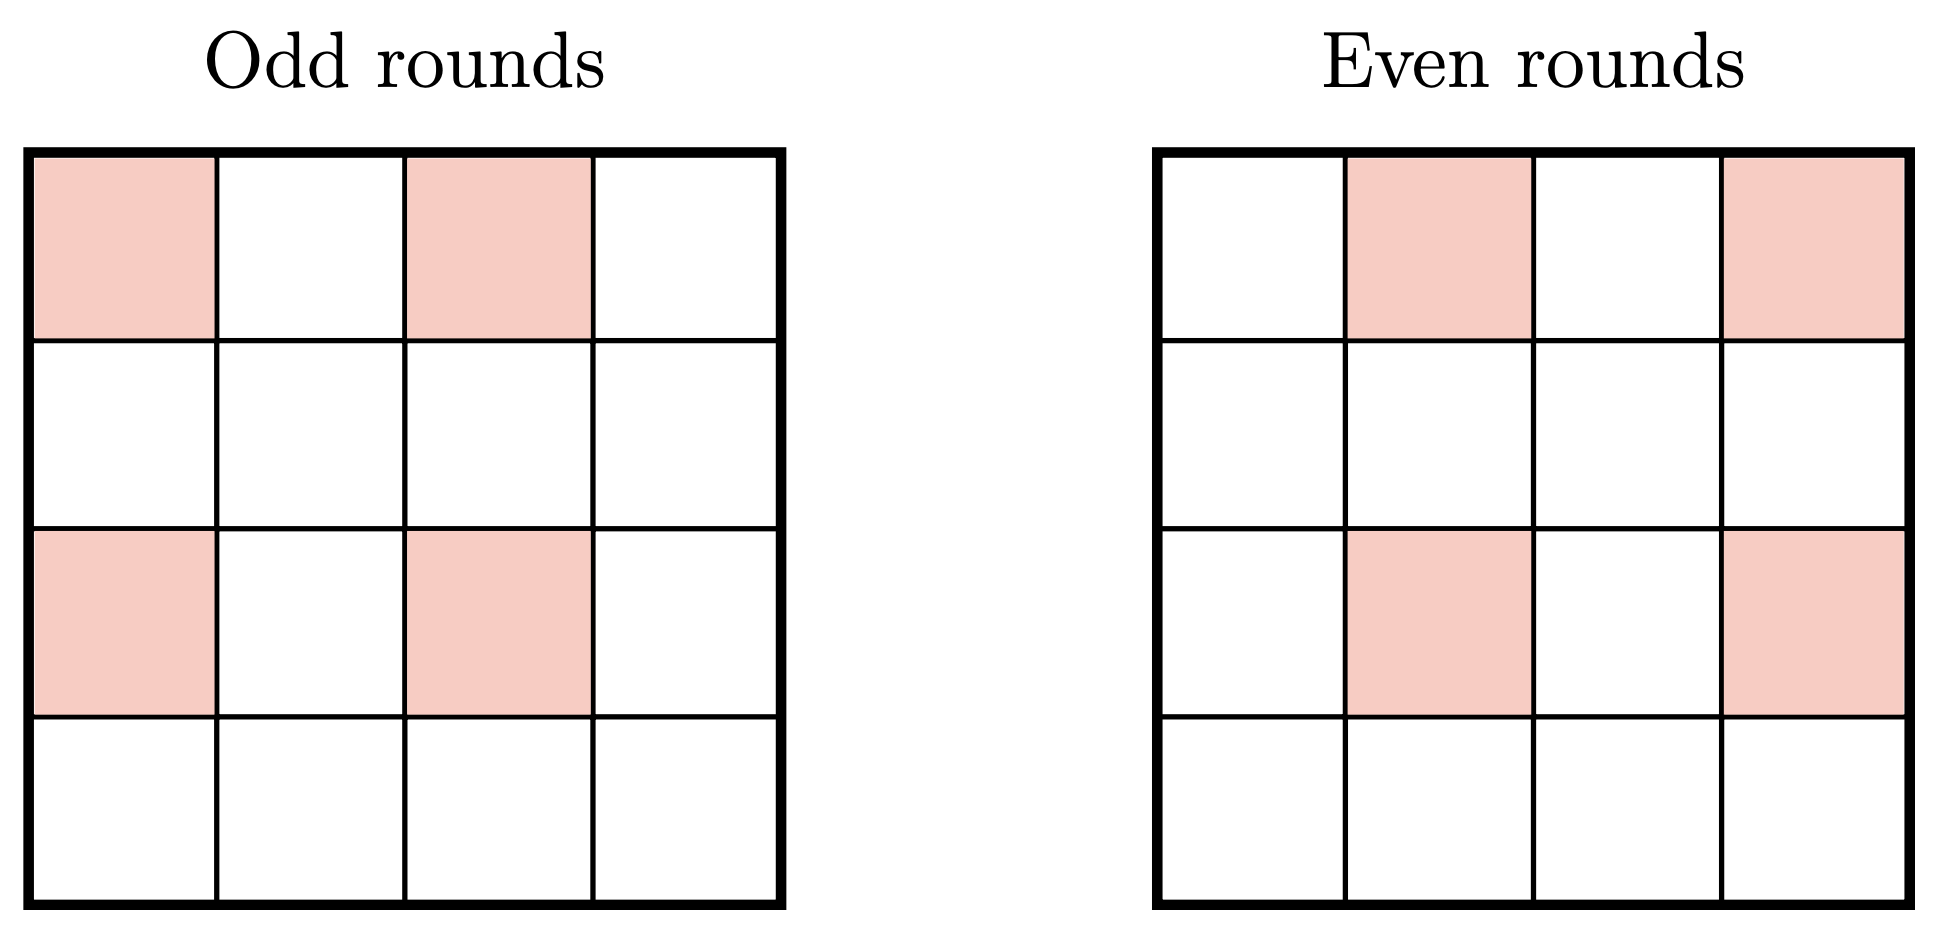
\includegraphics[width=7cm]{figures/lex.png}
  \caption{Extraction of internal state words for odd and even rounds of {\tt LEX}\label{fig:lex}. The extracted words are the ones being colored.}
\end{figure}

In 2008, Dunkelman and Keller presented an attack against LEX~\cite{AC:DunKel08b} able to recover the 128-bit secret key with $2^{36.3}$ bytes of key-stream produced by the same key and a time complexity of $2^{112}$ simple operations. This attack worked by exploiting a particular difference pattern of probability $2^{-64}$ in the {\tt \gls{AES}} internal state that could be detected by observing a $32$-bit condition in the output key stream.  The attack can be decomposed  in the three following steps:
\begin{enumerate}
\item  The attacker observes the output stream for a specific 32-bit pattern to occur (the four output words at a certain round should all be zero). This potentially indicates a special difference pattern (8 particular words with zero-difference) in the internal state of {\tt \gls{AES}}. 
\item Once this difference pattern is detected, the attacker recovers the values of 16 bytes of the internal state in both {\tt \gls{AES}} encryptions. This is achieved by guessing the difference in eight additional state words and by exploiting simple properties of the  {\sf MixColumns} and the  S-box. 
\item Finally, using the recovered 16 bytes, the attacker proceeds with a guess-and-determine approach to retrieve the secret key. The key step here is exploiting relations derived from the {\tt \gls{AES}-128} key schedule that link bytes from three consecutive subkeys, reducing the number of required guesses to just two subkey bytes. This limits the guessing process to only 10 bytes (80 bits) in total.
\end{enumerate}

\coolName{}'s structure ressembles {\tt LEX} in several aspects, the most notable being the extraction of four words at each iteration. Additionally, \coolName{}'s round function is inspired by the {\tt \gls{AES}} round function. For these reasons, it is natural to question whether the attack described in~\cite{AC:DunKel08b} could be adapted to \coolName{}. However, as we will argue next,  \coolName{} differs from {\tt LEX} in some crucial design choices, making the Dunkelman and Keller attack very difficult to apply:

\begin{itemize}
\item The output of the FSM at every round is masked by the whitening LFSR $\mathcal{W}$ making it hard to directly recover the values of the internal state as done in the attack of {\tt LEX}.
\item The LFSR $\mathcal{K}$ playing the role of the key schedule, produces uncorrelated outputs, making it hard to find simple relations between key values in consecutive rounds. A crucial element in the success of the attack against {\tt LEX} was exactly the fact that by guessing only two key bytes, the attacker was able to recover many more key values by exploiting such relations holding over several rounds. As we showed in the previous sections, it is not possible for an attacker to extract any information on the secret key by observing the output of the FSM over 3 or 4 consecutive rounds. 
\end{itemize}


\subsection{Truncated Linear Trails from MILP}
\label{sec:milp}


In order to find a lower bound for the number of S-boxes active in a linear trail over 4 rounds of \coolName, we apply the approach introduced by Mouha \emph{et al.\@}~\cite{add:MWGP11} in the most direct way. As we are interested in the (in)activity of the Sboxes throughout the rounds, we only need to assign binary variables to output digits, but also to internal digits of the state before the S-box layer, and before the MixColumn operation. For each round, we then have $4 + 16 + 16 = 36$ binary variables that are related one to others by the following constraints.
\begin{description}
\item[3-fork constraint.] Any output digit corresponds to a digit of the internal state after the S-box layer, so it is naturally related to the activity of a digit before MixColumn, by taking care of the reorganization of the digits through ShiftRows. But because the activity pattern is unchanged through the S-box layer, it is also related to a digit before the S-box layer. The constraint between three such variables is that if one is active, then at least two of them are. This corresponds to a 3-fork constraint that can be modeled as in \cite[Sec~ 2.2]{add:MWGP11}.
\item[MDS constraint.] A given column before and after MixColumns are related by the following MDS constraint: if a digit is active, then at least 5 of them are. This can be modeled in a manner similar to the 3-fork. In our case, the binary variables associated to the state after MixColumns at round $r$ are the one corresponding to the state before the S-box layer at round $r+1$.
\item[Border constraints.] We also add some border constraints to ensure that the initial inner state is fully inactive, and that the same holds for the final inner state. This way, we make sure that the considered linear equations do not depend on the unknown FSM state, but only on the key and output digits. We also impose that at least a digit among the ones output at the first round, and at least one among the ones of the last round must be active.
\end{description}
Finally, with the described constraints, the objective is to minimize the number of active Sboxes, that is, the number of active digits before the S-box layer. Note that any solution to this problem is actually a worst-case scenario in our case: a returned activation pattern is not guaranteed to be actually instantiable. We solved this simple MILP model using the SageMath interface for Mixed Integer Linear Programing solving within seconds on a standard laptop. Our code is 
\ifeprint
  available online.\footnote{\url{https://github.com/CryptoExperts/Transistor/}}
\else
  provided as supplementary material.
\fi

Most notably, we have found that
\[w_4 \geq 13,\  w_5 \geq 20 \mbox{ and } w_6 \geq 25\]
with the potential trail examples depicted on Fig.~\ref{fig:trails}.
We also verified that \(w_n \geq 26\) for $n \in \{7, 8, \ldots 26\}$.
For larger values of $n$, either a trail has at least one active S-box per
round, or it splits into two smaller trails with at least 13 active
Sboxes.  Therefore, we deduce that \(w_n \ge 26\) for all $n \ge 7$.

\begin{figure}[h]
  \centering
  \begin{subfigure}[t]{0.22\textwidth}
    \centering
    \includegraphics[scale=.55]{figures/solution_0.pdf}
    \caption{4-round trail.}
  \end{subfigure}
  \hfill
  \begin{subfigure}[t]{0.22\textwidth}
    \centering
    \includegraphics[scale=.55]{figures/solution_1.pdf}
    \caption{4-round trail.}
  \end{subfigure}
  \hfill
  \begin{subfigure}[t]{0.22\textwidth}
    \centering
    \includegraphics[scale=.55]{figures/solution_2.pdf}
    \caption{4-round trail.}
  \end{subfigure}
  \hfill
  \begin{subfigure}[t]{0.22\textwidth}
    \centering
    \includegraphics[scale=.55]{figures/solution_3.pdf}
    \caption{4-round trail.}
  \end{subfigure}
  
  \begin{subfigure}[t]{0.45\textwidth}
    \centering
    \includegraphics[scale=.6]{figures/milp_5.pdf}
    \caption{5-round trail.}
  \end{subfigure}
  \caption{Activity patterns for linear trails over 4 and 5 rounds.}
  \label{fig:trails}
\end{figure}

%\ac{Donner les figures des 4 trails tronques pour \(4\) tours ici.}


% Leo: ce qui suit est pour qu'emacs compile bien l'article, pas touche !
%%% Local Variables:
%%% mode: latex
%%% ispell-local-dictionary: "english"
%%% TeX-master: "main"
%%% End:

